\documentclass[11pt, dvipsnames, DIV=12]{scrreprt}
\usepackage{babel}

\usepackage[utf8]{inputenc}
\usepackage[T1]{fontenc}
\usepackage{natbib}
\bibliographystyle{abbrvnat}
\usepackage{subcaption}
\usepackage{booktabs}
\usepackage{multirow}
\usepackage{url}
\usepackage{tikz}
\usetikzlibrary{patterns,decorations.pathreplacing}
\usetikzlibrary{arrows.meta,arrows}
\usetikzlibrary{calc}




\usepackage{paralist}

\usepackage{ifthen}
\newcommand{\CC}[1][]{$\text{C\hspace{-.25ex}}^{_{_{_{++}}}}
\ifthenelse{\equal{#1}{}}{}{\text{\hspace{-.625ex}#1}}$}

\usepackage{bm}
\usepackage{amsmath}
\usepackage{amssymb}
\usepackage{amsthm}
\usepackage{amsfonts}
\usepackage{thmtools}		
\usepackage{mleftright}
\usepackage{stmaryrd}
\usepackage{nicefrac}
\usepackage{algorithm}
\usepackage{algorithmicx}
\usepackage[noend]{algpseudocode}
\renewcommand{\algorithmicrequire}{\textbf{Input:}}
\renewcommand{\algorithmicensure}{\textbf{Output:}}

\usepackage{dsfont} % For the indicator function: \mathds{1}


% Fixes some spacing issues with braces.
\let\originalleft\left
\let\originalright\right
\renewcommand{\left}{\mathopen{}\mathclose\bgroup\originalleft}
\renewcommand{\right}{\aftergroup\egroup\originalright}

\theoremstyle{definition}
\newtheorem{theorem}{Theorem}
\newtheorem{conjecture}{Conjecture}
\newtheorem{proposition}[theorem]{Proposition}
\newtheorem{insight}{Insight}
\newtheorem{observation}{Observation}
\newtheorem{lemma}[theorem]{Lemma}
\newtheorem{corollary}[theorem]{Corollary}
\newtheorem{definition}[theorem]{Definition}
\newtheorem{example}[theorem]{Example}
\newtheorem{remark}[theorem]{Remark}
\newtheorem{claim}[theorem]{Claim}
\newtheorem{fact}[theorem]{Fact}
\usepackage{thm-restate}
\usepackage[mathic=true]{mathtools}
\usepackage{fixmath}
\usepackage{siunitx}

\usepackage{pifont}
\newcommand{\cmark}{\ding{51}}
\newcommand{\xmark}{\ding{55}}
\usepackage{blindtext}

\usepackage{todonotes}

\usepackage{enumitem}
\setlist[enumerate]{itemsep=0.2ex, topsep=0.5\topsep}
\setlist[description]{itemsep=0.2ex, topsep=0.5\topsep}
\setlist[itemize]{itemsep=0.2ex, topsep=0.5\topsep}


% Let cleveref and thmtools work together
\makeatletter
\def\thmt@refnamewithcomma #1#2#3,#4,#5\@nil{%
\@xa\def\csname\thmt@envname #1utorefname\endcsname{#3}%
\ifcsname #2refname\endcsname
\csname #2refname\expandafter\endcsname\expandafter{\thmt@envname}{#3}{#4}%
\fi
}
\makeatother

% Removed 'pagebackref,' as it makes the bilbipgraphy more cluddered in my opinion
\usepackage[
pdfa,
hidelinks,
pdftex, 
pdfdisplaydoctitle,
pdfpagelabels,
pdfauthor={},
pdftitle={},
pdfsubject={},
pdfkeywords={},
pdfproducer={Latex with the hyperref package},
pdfcreator={pdflatex}
]{hyperref}

\usepackage[capitalise,noabbrev]{cleveref}   

\usepackage{microtype}
\usepackage{ellipsis}

\usepackage[scaled=0.86]{helvet}
\usepackage{lmodern}

\usepackage{pgfplots}

% Bold. 
\newcommand{\mF}{\mathbf{F}}
\newcommand{\mG}{\mathbf{G}}
\newcommand{\mH}{\mathbf{H}}
\newcommand{\mL}{\mathbf{L}}
\newcommand{\mI}{\mathbf{I}}

\newcommand{\mW}{\mathbf{W}}
\newcommand{\ma}{\mathbf{a}}
\newcommand{\mb}{\mathbf{b}}
\newcommand{\mw}{\mathbf{w}}

\newcommand{\ba}{\ensuremath{{\bf a}}}
\newcommand{\bb}{\ensuremath{{\bf b}}}
\newcommand{\bc}{\ensuremath{{\bf c}}}

% Calligraphic.
\newcommand{\cA}{\mathcal{A}}
\newcommand{\cB}{\mathcal{B}}
\newcommand{\cC}{\mathcal{C}}
\newcommand{\cF}{\mathcal{F}}
\newcommand{\cG}{\mathcal{G}}
\newcommand{\cH}{\mathcal{H}}
\newcommand{\cN}{\mathcal{N}}
\newcommand{\cO}{\mathcal{O}}
\newcommand{\cP}{\mathcal{P}}
\newcommand{\cR}{\mathcal{R}}
\newcommand{\cS}{\mathcal{S}}
\newcommand{\cT}{\mathcal{T}}
\newcommand{\cU}{\mathcal{U}}
\newcommand{\cV}{\mathcal{V}}
\newcommand{\cX}{\mathcal{X}}


% Sans serif.
\newcommand{\sC}{\mathsf{C}}

% Blackboard.
\newcommand{\Fb}{\mathbb{F}}
\newcommand{\Gb}{\mathbb{G}}
\newcommand{\Nb}{\mathbb{N}}
\newcommand{\Qb}{\mathbb{Q}}
\newcommand{\Rb}{\mathbb{R}}
\newcommand{\Zb}{\mathbb{Z}}

% Multiset Definition
\newcommand{\MSopen}{\{\!\!\{}
\newcommand{\MSclose}{\}\!\!\}}

% 1-WL+NN
\newcommand{\wlnn}{\text{1-WL+NN}}
\newcommand{\wliso}{\simeq_{\text{1WL}}}
\newcommand{\knn}{K^{n \times n}}
\newcommand{\gapp}{\text{GNN-Approximating}}
\newcommand{\wldisc}{\text{1-\!WL-Discriminating}}
\newcommand{\wl}{\text{1-\!WL}}
\newcommand{\mlp}{\text{MLP}}

%Parameter for sampling, keep low for fast compile times, and inrease when submitting the work
\def\samples{5}


\usepackage[auth-lg]{authblk}
\newcommand{\cm}[1]{{{\textcolor{purple}{\textbf{[CM:} {#1}\textbf{]}}}}}


\renewcommand*{\Affilfont}{\large\normalfont}
\renewcommand*{\Authfont}{\normalfont}

\recalctypearea
\setcounter{Maxaffil}{2}

\title{A Theoretical and Empirical Investigation into the Equivalence of Graph Neural Networks and the Weisfeiler-Leman Algorithm\\
\vspace{20pt}\small{\normalfont From the faculty of Mathematics, Physics, and Computer Science approved for the purpose of obtaining the academic degree of Bachelor of Sciences.}
}
\author{\textbf{Eric Tillmann Bill}}
\affil{\vspace{100pt}}

\author{Supervision:\\Prof. Dr. rer. nat. Christopher Morris}
\affil{Informatik 6\\RWTH Aachen University}

\date{\vspace{-30pt}}

\renewcommand{\thesection}{\arabic{section}}

\begin{document}

\maketitle
\tableofcontents
\newpage
\section{Introduction}
This work aims to shed light on the representations learned by \textsf{Graph Neural Networks}. In this section, we will discuss the prevalence of graphs and the crucial role \gnns play in analyzing them. We will delve into the methods we use to gain insights and highlight the significance of our approach. Lastly, we will provide an overview of the structure of this work.

\subsection{Motivation}
Graphs are ubiquitous in various fields of life. Despite not always being explicitly identified as such, the graph data model's flexibility and simplicity make it an effective tool for modeling a diverse range of data. Examples of graph modeling applications include unexpected instances, such as modeling text or images as a graph, as well as more complex instances like chemical molecules, citation networks, or connectivity encodings of the World Wide Web \cite{Mor+2020, Sca+2009}.

Although machine learning has achieved remarkable success with image classification (e.g., \cite{Zoph2018, He2016}) and text generation (e.g., \cite{Radford2019, Brown2020}) in the last decade, the lack of a significant breakthrough in machine learning for graphs can be attributed to the graph data model's inherent flexibility and simplicity. While, for example, an image classifier constrains its input data to be a grid-like image or a text generator expects its input to be a linear sequence of words, machine learning models working on graphs cannot leverage any constraints on the format or size of their input graphs without limiting their generality. 

To put this flexibility of the graph data model into perspective and give an idea of how ubiquitous graphs are in various fields, we refer back to the examples of image classifiers and text generators and demonstrate how seemingly natural the graph data model can encode their input data. For example, images can be encoded by a graph, such that each pixel of the image corresponds to a node in the graph holding its color value, and each node is connected to its neighboring pixel nodes. Similarly, for sequential data like text files, one can encode a directed graph where each word in this file is represented as a node with the word as a feature and connected outgoingly to the next following word. See \cref{fig:example_encodings} for an illustrative example of these encodings.

In recent years, a significant amount of research has been conducted to investigate \textsf{Graph Neural Networks} (\gnns). Among the most promising approaches are those utilizing the message-passing architecture, which was introduced by \cite{Sca+2009} and \cite{Gil+2017}. 
Empirically, this framework has demonstrated strong performance across various applications \cite{Kip+2017, Ham+2017, Xu2018}. However, its expressiveness is limited, as has been proved by the works of \cite{Morris2018}, as well as \cite{Xu2018}. These works establish a connection to the \textsf{Weisfeiler-Leman}\footnote{Based on \href{https://www.iti.zcu.cz/wl2018/pdf/leman.pdf}{https://www.iti.zcu.cz/wl2018/pdf/leman.pdf}, we will use the spelling ``Leman'' here, as requested by A. Leman, the co-inventor of the algorithm.} algorithm (\wl), originally proposed by \cite{Wei+1968} as a simple heuristic for the graph isomorphism problem. In particular, it has been proven that a \gnn based on the message-passing architecture can, at most, be as good as the \wl algorithm in distinguishing non-isomorphic graphs. Furthermore, the \wl method demonstrates numerous similarities with the fundamental workings of the \gnn architecture. It is, therefore, commonly believed that both methods are, to some extent, equivalent in their capacity to capture information in a graph.

Despite the remarkable empirical performance of \gnns, particularly compared to conventional graph kernel functions \cite{Mor+2020}, and the theoretical understanding of their ability to distinguish non-isomorphic graphs, there remains a limited understanding of the learned representations that drive this empirical success. This work aims to delve into these representations, seeking deeper insights into the factors contributing to the efficacy of \gnns.

\begin{figure}[!t]
 \centering
 \begin{subfigure}[b]{0.475\textwidth}
    \centering
    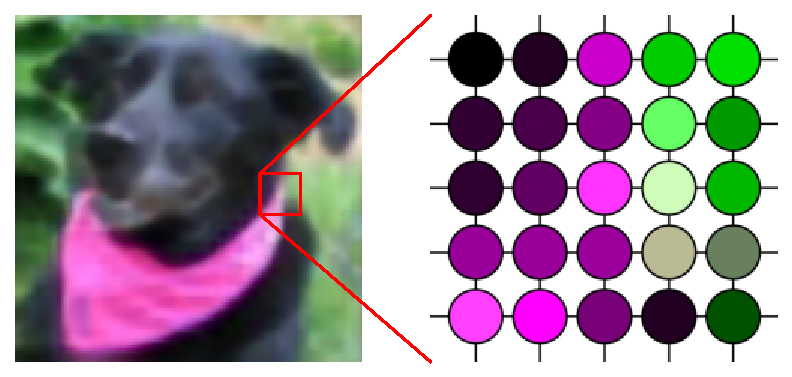
\includegraphics[width=\textwidth]{Figures/encoding_example.pdf}
    \caption{Graph Encoding of an Image\footnotemark}
 \end{subfigure}
 \hfill
 \begin{subfigure}[b]{0.475\textwidth}
    \centering
    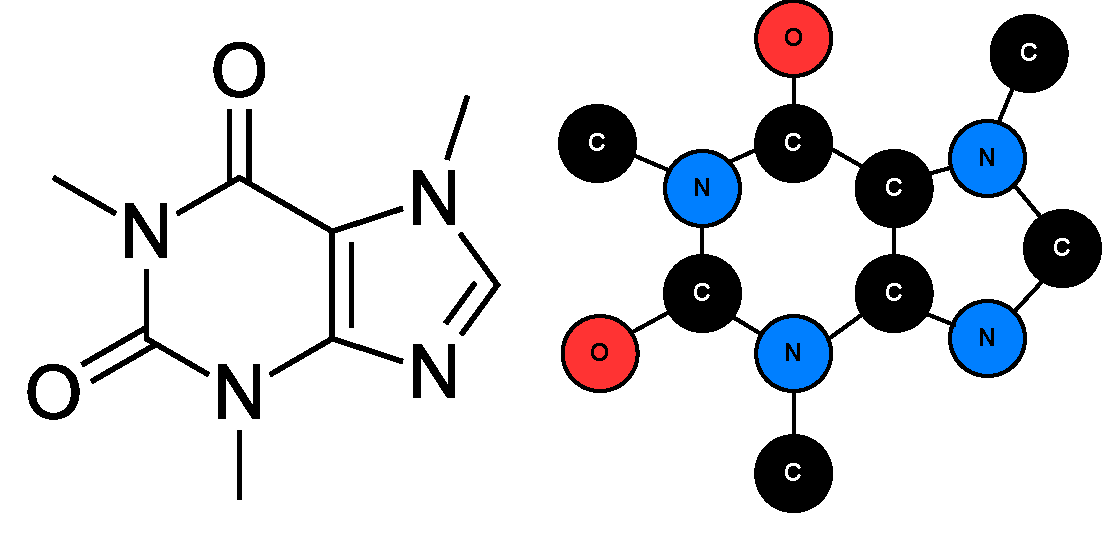
\includegraphics[width=\textwidth]{Figures/Example_Encoding_Molecule.pdf}
    \caption{Graph Encoding of a Molecule\footnotemark}
 \end{subfigure}
 \par\medskip
 \begin{subfigure}[b]{0.475\textwidth}
    \centering
    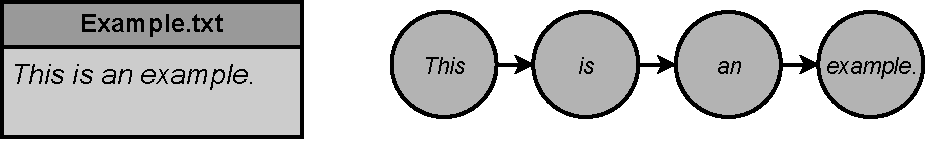
\includegraphics[width=\textwidth]{Figures/Example_Encoding_Text.pdf}
    \caption{Graph Encoding of a Text File.}
 \end{subfigure}
 \caption[Caption for LOF]{An overview of three examples of how graphs can be used to encode information across different domains. For each example, the conventional domain-specific encodings are visualized on the left, while on the right, we showcase how a graph can encode the same information. Note that these examples are just a sample; in actual practice, more detailed encodings are usually utilized to capture additional information.\footnotemark}
 \label{fig:example_encodings}
\end{figure}\todo{Footnotes are wrong!}
\footnotetext[2]{The image of a dog is from the CIFAR-10 collection made available by \cite{Krizhevsky2009}.}
\footnotetext[3]{The illustration of the skeletal formula of caffeine is taken from \href{https://commons.wikimedia.org/wiki/File:Caffeine_structure.svg}{https://commons.wikimedia.org}.}
\footnotetext{All graphics were created using the free open source platform \href{https://www.draw.io}{https://www.draw.io}.}

\subsection{Methology}
In this work, we introduce a novel framework, which we coined ``\wlnn,'' which involves applying the \wl algorithm to an input graph and further processing the resulting information using a feedforward neural network. Thereby, we obtain a trainable framework suited for all kinds of graph-related tasks, such as graph classification, node regression, and more. We will prove that both frameworks, \wlnn and \gnn, are theoretically equivalent, such that each function computed by a \wlnn model can also be computed by a \gnn model and vice versa. With this framework in hand, we can investigate the representations learned by a \gnn.

The interesting property of this framework compared to \gnns, which is also the original idea that inspired this work, is the fundamental difference in how both frameworks learn and optimize themselves when applied to a specific task. Take, for example, an arbitrary classification task. While the first part of a \wlnn model starts by applying the \wl algorithm to its input graph and retrieves a highly informative representation of this graph, the second part, the learnable feedforward neural network, must find common patterns in this very detailed representation that coincides with the class labels of the task, such that the model makes good predictions. In contrast, a \gnn first must learn how to process the information in a graph effectively and then find common patterns in its computed representation that correlate with the class labels so that the model can make good predictions.

To put both learning behaviors into perspective on a high level, while a \wlnn model is given a maximally informative representation and needs to find the essential information in this representation to make a good prediction, a \gnn works the other way around since it first has to learn how to effectively compute good representations of a graph and then leverage this information for good predictions. Despite their difference in learning behaviors, both methods can compute the same functions, making a fascinating comparison of their empirical performance.

Therefore, we will use this novel framework and various empirical experiments to compare both frameworks on multiple datasets to establish a deeper understanding of the representations learned by \gnns.

\subsection{Research Questions \& Contributions}
\begin{enumerate}
   \item \wlnn as a framework for analyzing \gnns. We will show the theoretical equivalence and show that both methods share many emprical similarities, such that this tool is a great for analyzing various aspects of a \gnn.
   \item We will show
\end{enumerate}

\subsection{Outline}
For ease of readability, we split this work into two parts. The first part investigates and establishes the theoretical equivalence between the frameworks of \wlnn and \gnns. In contrast, the second part presents our different experiments and their empirical results, in which we use the \wlnn framework as a tool to analyze the representation learned by a \gnn.

In detail, this work starts with \cref{sec:related_work}, where we discuss related work, milestones in \gnns over the past decade, essential properties of the \wl algorithm, and a subset of interesting connections between \gnns and the \wl algorithm.

Afterward, we will start with \cref{part1}, which begins with \cref{sec:pre_lim}. Here, we will introduce formal definitions for both frameworks, as well as a set of notations we will use throughout the theoretical part. Preceding, in \cref{sec:theo_connections}, we will introduce two theorems that each present a connection between both frameworks and combined prove the equivalence of both frameworks. Finally, we will prove each theorem individually after another in corresponding subsections.

The second part is dedicated to our empirical experiments. We begin with \cref{sec:testing_configuration}, explaining the experimental setup and our experiment choices. In detail, we will discuss the choice of benchmarking datasets, \gnn models, and \wlnn models, along with an explanation of our general testing procedure. In \cref{sec:emprical_results}, we present the results of our experiments and delve into further analyses of certain aspects of \gnn and \wlnn models. In particular, we will investigate the representations computed by \gnns and try to infer common patterns that occurred across multiple datasets. Finally, the thesis concludes with a final discussion in \cref{sec:discussion}, where we summarize our findings, address the limitations of this work, and offer recommendations for future research.
\section{Related Work}
Yet to come!
\newpage
This part of the thesis focuses on the equivalence between \wlnn and \gnn. We will begin by providing a preliminary section that formalizes all the concepts used in the proof and introduces a general notation. Afterward, we will dedicate a separate section to present and prove three theorems. These theorems combined conclude the equivalence.

\section{Preliminaries}\label{sec:pre_lim}
This section will introduce and formalizes all concepts used throughout the proof and the rest of the thesis. We start with general notations, introduce a general graph definition, and familiarize the reader with the Weisfeiler-Leman algorithm. We will introduce each framework independently, first the \wlnn and then \gnn. In the end, we will briefly introduce important properties of collections of functions computed by both methods.

\subsection{General Notation}
Let $\Nb$ denote the set of natural numbers such that $\Nb := \{0, 1,2, \ldots \}$. By $[n]$, we denote the set $\{0, \ldots, n\} \subset \mathbb{N}$ for each $n \in \mathbb{N}$. Further, with $\MSopen \ldots \MSclose$, we denote a multiset formally defined as a 2-tuple $(X, m)$, where $X$ is a set of all unique elements and $m: X \rightarrow \mathbb{N}_{\geq 1}$ a mapping that maps each element in $X$ to the number of its occurrences in the multiset.

\subsection{Graphs}
We will briefly introduce a formal definition for graphs and coloring on graphs. Starting with the definition of a graph.

\begin{definition}[Graph]
A graph $G$ is defined as a 3-tuple denoted by $G \coloneqq (V, E, l)$. This tuple consists of a set of nodes $V \subset \Nb$, a set of edges $E \subseteq V \times V$, and a labeling function $l: M \rightarrow \Sigma$. The domain $M$ of the labeling function can be either $V$, $V \cup E$, or $E$, and the codomain $\Sigma$ is an alphabet with $\Sigma \subseteq \mathbb{N}^k$, where $k \in \Nb$ is arbitrary.
In the context of this thesis, the assigned values by the labeling function are referred to as either labels or features, depending on the dimension of $\Sigma$. In detail, if $k=1$, we usually refer to the values as labels, otherwise as features. Additionally, the set of all graphs is denoted by $\cG$.

Furthermore, a graph $G$ can be either directed or undirected based on the definition of its set of edges $E$. If $E \subseteq \{(v,u) \mid v,u \in V\}$, it represents a directed graph, whereas if $E \subseteq \{(v, u) \mid v,u \in V, v\neq u\}$ such that for every $(v,u) \in E$ there exists $(u,v) \in E$, it defines an undirected graph. Additionally, for ease of notation, we will use $V(G)$ and $E(G)$ to denote the set of nodes and the set of edges of $G$, respectively, as well as $l_G$ to denote the label function of $G$. Further, with $\mathcal{N}(v)$ for $v \in V(G)$ we denote the set of neighbors of $v$ defined as $\mathcal{N}(v) \coloneqq \{u \mid (u, v) \in E(G)\}$, and with $d(v)$ for $v \in V(G)$ the degree of node $v$, defined as $d(v) := |\mathcal{N}(v)|$.
\end{definition}

We continue with the definition of a graph coloring.

\begin{definition}[Graph Coloring]
A coloring of a Graph $G$ is a function $C: V(G) \rightarrow \mathbb{N}$ that assigns each node in the graph a color (here, a positive integer). Further, a coloring $C$ induces a partition $\cP$ on the set of nodes, for which we define $C^{-1}$ being the function that maps each color $c \in \mathbb{N}$ to its class of nodes with $C^{-1}(c) = \{ v\in V(G) \mid C(v) = c\}$. In addition, we define $\hist_{G, C}$ as the histogram of graph $G$ with coloring $C$ that maps every color in the image of $C$ under $V(G)$ to the number of occurrences. In detail, $\forall c \in \mathbb{N}: \hist_{G, C}(c) \coloneqq | \{ v \in V(G) \mid C(v) = c \} | = | C^{-1}(c) |$.
\end{definition}

\subsubsection{Permutation-invariance and -equivariance}
We use $S_n$ to denote the symmetric group over the elements $[n]$ for any $n \in \Nb$. $S_n$ consists of all permutations over these elements. Let $G$ be a graph with $V(G) = [n]$, applying a permutation $\pi \in S_n$ on $G$, is defined as $G_\pi \coloneqq \pi \cdot G$ where $V(G_\pi) = \{\pi(0), \ldots, \pi(n) \}$ and $E(G_\pi) = \{ (\pi(v), \pi(u)) \mid (v,u) \in E(G)\}$. We will now introduce two key concepts for classifying functions on graphs.

\begin{definition}[Permutation Invariant]
    Let $f: \mathcal{G} \rightarrow \mathcal{Y}$ be an arbitrary function, then $f$ is \textit{permutation-invariant} if and only if for all $G \in \mathcal{G}$, where $n_G \coloneqq |V(G)|$ and for every $\pi \in S_{n_G}$: $f(G) = f(\pi \cdot G)$.
\end{definition}

\begin{definition}[Permuation Equivariant]
    Let $f: \mathcal{G} \rightarrow \mathcal{Y}$ be an arbitrary function, then $f$ is \textit{permuation-equivariant} if and only if for all $G \in \mathcal{G}$, where $n_G \coloneqq |V(G)|$ and for every $\pi \in S_{n_G}$: $f(G) = \pi^{-1} \cdot f(\pi \cdot G)$.
\end{definition}

\subsection{Weisfeiler and Leman Algorithm}\label{sec:1-WL Definition}
The Weisfeiler-Leman algorithm consists of two main parts: the coloring algorithm and the graph isomorphism test. We will introduce each part individually and present some implications afterward.

\subsubsection{The Weisfeiler-Leman Graph Coloring Algorithm}
The $\wl$ algorithm computes a node coloring of its input graph in each iteration. In detail, a color is assigned to each node based on the colors of its neighbors and its own current color. The algorithm continues until convergence is reached, resulting in the final coloring of the graph. We will now formally define this procedure and provide an illustrative example in \cref{fig:1wl_example}.

\begin{definition}[$\wl$ Algorithm]
    Let $G = (V, E, l)$ be a labeled graph. In each iteration $i$, the \wl algorithm computes a node coloring $C_i: V(G) \rightarrow \mathbb{N}$. In the initial iteration $i=0$, the coloring is set to $C_0 = l$ if $l$ exists. Otherwise, for all $v \in V(G): C_0(v) = c$ with $c \in \Nb$ being an arbitrary but fixed constant. For $i > 0$, the algorithm assigns a color to $v \in V(G)$ as follows:
    \begin{equation*}
        C_i (v) = \textsf{RELABEL}(C_{i-1}(v),  \ \MSopen C_{i-1}(u) \mid u \in \mathcal{N}(v) \MSclose),
    \end{equation*}
    where $\textsf{RELABEL}$ injectively maps the above pair to a unique, previously not used, color. The algorithm terminates when the number of colors between two iterations does not change, meaning the algorithm terminates after iteration $i$ if the following condition is satisfied:
    \begin{equation*}
        \forall v,w \in V(G):  C_i(v) = C_i(w) \iff C_{i+1}(v) = C_{i+1}(w).
    \end{equation*}
    Upon terminating we define $C_{\infty} \coloneqq C_i$ as the stable coloring, such that $\wl(G) \coloneqq C_\infty$.
\end{definition}

The colorings computed in each iteration always converge to the final one, such that the algorithm always terminates. In more detail, \cite{Gro2017} showed that it always holds after at most $|V(G)|$ iterations. For an illustration of this algorithm, see \cref{fig:1wl_example}. Moreover, based on the work of \cite{Pai+87} about efficient refinement strategies, \cite{Car+82} proved that the stable coloring $C_\infty$ can be computed in time $\mathcal{O}(| V(G) | + |E(G)| \cdot \log | V(G) |)$.

\begin{figure}[H]
    \centering
    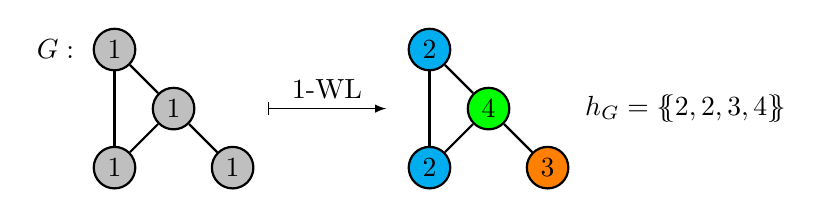
\begin{tikzpicture}
    \tikzset{line/.style={draw,thick}}
    \tikzset{arrow/.style={line,->,>=stealth}}
    \tikzset{node/.style={circle,inner sep=0pt,minimum width=15pt}}
    
    \draw (-1.5,0.75) node {$G:$};
    \node[line,node,fill=lightgray] (x1) at (-0.75, 0.75) {1};
    \node[line,node,fill=lightgray] (x2) at (-0.75, -0.75) {1};
    \node[line,node,fill=lightgray] (x3) at (0.75, -0.75) {1};
    \node[line,node,fill=lightgray] (x4) at (0, 0) {1};
    
    \path[line] (x1) to (x2);
    \path[line] (x1) to (x4);
    \path[line] (x2) to (x4);
    \path[line] (x3) to (x4);

    \draw [|-latex] (1.2,0) -- node [text width=2.5cm,midway,above,align=center ] {1-WL} (2.7,0);
    

    \node[line,node,fill=cyan] (x1) at (-0.75 + 4.0, 0.75) {2};
    \node[line,node,fill=cyan] (x2) at (-0.75 + 4.0, -0.75) {2};
    \node[line,node,fill=orange] (x3) at (0.75 + 4.0, -0.75) {3};
    \node[line,node,fill=green] (x4) at (0 + 4.0, 0) {4};
    
    \path[line] (x1) to (x2);
    \path[line] (x1) to (x4);
    \path[line] (x2) to (x4);
    \path[line] (x3) to (x4);

    \draw (6.5, 0.0) node {$h_G = \MSopen 2, 2, 3, 4 \MSclose$};

    
    
    \end{tikzpicture}

    \caption{An example of the final coloring computed by applying the \wl algorithm on the graph $G$. The graph $G$ consists of $4$ nodes with all their labels being set to the same color.}
    \label{fig:1wl_example}
\end{figure}

It is important to understand that since the algorithm was originally developed as a simple heuristic for the \textit{graph isomorphism problem}, which is an inherently discrete problem, the \wl algorithm in its simplest form, as we presented it here, does only work on graphs with discrete, one-dimensional node labels. Although it is quite easy to adapt the algorithm to respect discrete edge labels of a graph by using them as weights in the neighborhood aggregation (\cite{Shervashidze2011}), modifying its definition to work with continuous graph features is more complex. Numerous proposed modifications have been put forward to address this integration in the literature, such as those discussed by \cite{Mor+2016}. However, note that this particular topic will not be further investigated in this thesis, although its mention holds value for \cref{part2}.

\subsubsection{The Weisfeiler-Leman Graph Isomorphism Test}
The isomorphism test uses the \wl coloring algorithm and is defined as follows.

\begin{definition}[$\wl$ Isomorphism Test]
    To determine if two graphs $G, H \in \mathcal{G}$ are non-isomorphic ($G \ncong H)$, one applies the \wl coloring algorithm on both graphs ``in parallel'' and checks after each iteration if the occurrences of each color are equal, else the algorithm would terminate and conclude non-isomorphic. Formally, the algorithm concludes non-isomorphic in iteration $i$ if there exists a color $c$ such that: 
    \begin{equation*}
        |\{ v \in V(G) \mid C_i(v) = c\} | \neq |\{ w \in V(H) \mid C_i(w) = c\} |.
    \end{equation*}
\end{definition}

Note that this test is only sound and not complete for the \textit{graph isomorphism problem}. Counterexamples can be easily constructed where the algorithm fails to distinguish non-isomorphic graphs. See \cref{1-WL Counter Example} for a straightforward example of where this test fails that was discovered and proven by \cite{Cai1992}.
\begin{figure}[H]
    \centering
    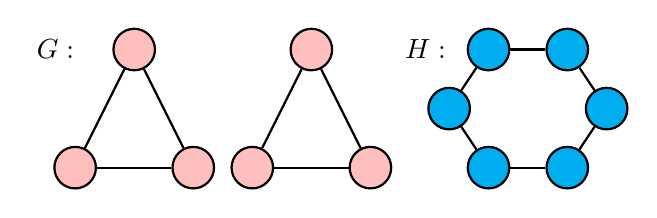
\begin{tikzpicture}

\tikzset{line/.style={draw,thick}}
\tikzset{arrow/.style={line,->,>=stealth}}
\tikzset{node/.style={circle,inner sep=0pt,minimum width=15pt}}

\draw (-1.0,0.75) node {$G:$};
\node[line,node,fill=pink] (x1) at (0, 0.75) {};
\node[line,node,fill=pink] (x2) at (-0.75, -0.75) {};
\node[line,node,fill=pink] (x3) at (0.75, -0.75) {};

\path[line] (x1) to (x2);
\path[line] (x1) to (x3);
\path[line] (x2) to (x3);

\node[line,node,fill=pink] (x1) at (2.25, 0.75) {};
\node[line,node,fill=pink] (x2) at (1.5, -0.75) {};
\node[line,node,fill=pink] (x3) at (3.0, -0.75) {};

\path[line] (x1) to (x2);
\path[line] (x1) to (x3);
\path[line] (x2) to (x3);

\draw (3.7, 0.75) node {$H:$};
\node[line,node,fill=cyan] (x1) at (3.75 + 0.25, 0) {};
\node[line,node,fill=cyan] (x2) at (4.25 + 0.25, 0.75) {};
\node[line,node,fill=cyan] (x3) at (5.25 + 0.25, 0.75) {};
\node[line,node,fill=cyan] (x4) at (5.75 + 0.25, 0) {};
\node[line,node,fill=cyan] (x5) at (5.25 + 0.25, -0.75) {};
\node[line,node,fill=cyan] (x6) at (4.25 + 0.25, -0.75) {};

\path[line] (x1) to (x2);
\path[line] (x2) to (x3);
\path[line] (x3) to (x4);
\path[line] (x4) to (x5);
\path[line] (x5) to (x6);
\path[line] (x6) to (x1);

\end{tikzpicture}
    \caption{This is an example of two graphs $G$ and $H$ that are non-isomorphic but cannot be distinguished by the \wl isomorphism test.}
    \label{1-WL Counter Example}
\end{figure}

\subsubsection{Implications of the \wl Algorithm}
One implication of the \wl algorithm and its isomorphism test is that, due to it not being complete for solving the \textit{graph isomorphism problem}, it gives rise to a related but weaker relation than the isomorphism relation ($\simeq$). We define this relation as follows.

\begin{definition}[\wl Relation]
    Let $\cX \subseteq \cG$. For any graphs $G,H \in \cX$ we will denote $G \wliso H$ if the \wl isomorphism test can not distinguish both graphs. Note that due to the soundness of this algorithm, if $G \not\wliso H$, we always can conclude that $G \not\simeq H$.
\end{definition}

The $\wliso$ relation can further be classified as an equivalence relation, as it is reflexive, symmetric and transitive. With this, we introduce a notation of its equivalence classes. Let $\cX \subseteq \cG$ and $G \in \cX$, then we denote with $\cX/\!{\wliso}(G): = \{ G' \in \cX \mid G \wliso G' \}$ its equivalence class.

Similarly, we define the notion \wldisc for collections of permutation invariant functions.

\begin{definition}[\wldisc]
    Let $\cX \subseteq \cG$. Further, let $\cC$ be a collection of permutation invariant functions from $\cX$ to $\Rb$. We say $\cC$ is \wldisc if for all graphs $G_1, G_2 \in \cX$ for which the \wl isomorphism test concludes non-isomorphic ($G_1 \not\wliso G_2$), there exists a function $h_{G_1, G_2} \in \cC$ such that $h_{G_1, G_2}(G_1) \neq h_{G_1, G_2}(G_2)$.
\end{definition}

\subsection{\wlnn}\label{sec:definition_wlnn}
As the \cref{sec:related_work_wl} shows, the $\wl$ algorithm is quite powerful in identifying a graph's substructures and distinguishing non-isomorphic graph pairs. With the \wlnn framework, we define functions that utilize this structural information to derive application-specific insights.

\begin{definition}[\wlnn]
    A \wlnn model consists of three components that are applied sequentially to its input: 1. the $\wl$ algorithm, 2. an encoding function $f_\text{enc}$ operating on graph colorings, and 3. an arbitrary multilayer perceptron $\mlp$. In detail, a \wlnn model computes the function $\cB$, that is defined as follows:
    \begin{align*}
        \cB: \cG \rightarrow \Rb^k, \ G \mapsto \mlp \circ f_{\text{enc}}(\MSopen \wl(G)(v) \mid v \in V(G) \MSclose),
    \end{align*}
    where $\wl(G)$ is the coloring computed by the $\wl$ algorithm when applied on $G$, and $k \in \Nb_{\geq 1}$ is a freely selectable hyperparameter. For a better understanding and an illustrative explanation, see \cref{fig:wlnn}.
\end{definition}

\begin{figure}[!htb]
    \centering
    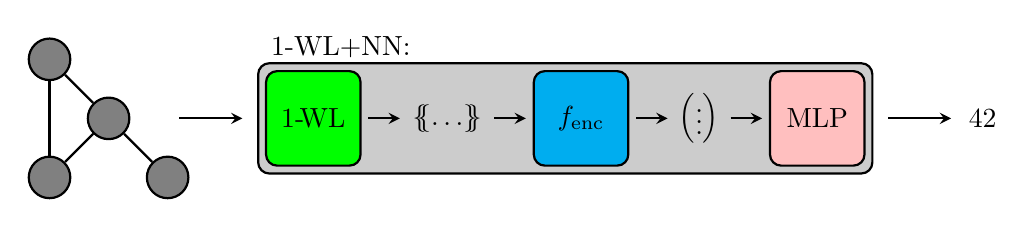
\begin{tikzpicture}
    \definecolor{pastell_blue}{RGB}{133,154,202}
    \definecolor{pastell_green}{RGB}{192,223,211}
    \definecolor{pastell_pink}{RGB}{228,197,212}
    \tikzset{line/.style={draw,thick}}
    \tikzset{arrow/.style={line,->,>=stealth}}
    \tikzset{node/.style={circle,inner sep=0pt,minimum width=15pt}}
    
    \node[line,node,fill=gray] (x1) at (-0.75 - 0.8, 0.75) {};
    \node[line,node,fill=gray] (x2) at (-0.75 - 0.8, -0.75) {};
    \node[line,node,fill=gray] (x3) at (0.75 - 0.8, -0.75) {};
    \node[line,node,fill=gray] (x4) at (0 - 0.8, 0) {};
    
    \path[line] (x1) to (x2);
    \path[line] (x1) to (x4);
    \path[line] (x2) to (x4);
    \path[line] (x3) to (x4);

    \draw[arrow, thick] (0.1, 0.0) to (0.9, 0.0);

    \draw (2.15, 0.9) node {$\wlnn$:};
    \filldraw[draw=black, fill=gray!40, thick, rounded corners] (1.1, -0.7) rectangle (8.9, 0.7);

    \filldraw[draw=black, fill=green, thick, rounded corners] (1.2, -0.6) rectangle (2.4, 0.6) node[midway,align=center]{$\wl$};

    \draw[arrow, thick] (2.5, 0.0) to (2.9, 0.0);
    
    \draw (3.5, 0.0) node {$\MSopen \ldots \MSclose$};

    \draw[arrow, thick] (4.1, 0.0) to (4.5, 0.0);

    \filldraw[draw=black, fill=cyan, thick, rounded corners] (4.6, -0.6) rectangle (5.8, 0.6) node[midway,align=center]{$f_{\text{enc}}$};

    \draw[arrow, thick] (5.9, 0.0) to (6.3, 0.0);
    \draw (6.7, 0.0) node {$\begin{pmatrix*} \vdots \end{pmatrix*}$};
    \draw[arrow, thick] (7.1, 0.0) to (7.5, 0.0);

    \filldraw[draw=black, fill=pink, thick, rounded corners] (7.6, -0.6) rectangle (8.8, 0.6) node[midway,align=center]{$\mlp$};

    \draw[arrow, thick] (9.1, 0.0) to (9.9, 0.0);
    \draw (10.3, 0.0) node {$42$};
    
\end{tikzpicture}

    \caption{This simplified illustration explains the components that make up a \wlnn model and how each one processes the input further. In detail, the model takes the graph on the left as input and first applies the \wl algorithm, thereby obtaining a multiset of the colors assigned by the algorithm. Then the encoding function $f_\text{enc}$ is applied, resulting in a fixed-sized vector that is further processed by the multilayer perceptron $\mlp$. The output of the $\mlp$ is then propagated as the \wlnn models output, here the number $42$.}
    \label{fig:wlnn}
\end{figure}

It is worth noting that this definition can be easily adjusted to accommodate node- or edge-level tasks by applying the encoding function $f_\text{enc}$ and the multilayer perceptron $\mlp$ elementwise to the colors of the multiset. However, for the purposes of this thesis, we will not delve into these variations, as our main focus will be on graph-level tasks such as graph classification or regression, which possess greater theoretical interest and are more prevalent in most datasets. Furthermore, all the theoretical findings presented in this thesis can be straightforwardly adapted to \wlnn models designed for node- or edge-level tasks.

\subsection{Graph Neural Networks (Message-Passing)}\label{sec:GNN Defintion}
A \textsf{Graph Neural Network} (\gnn) is a composition of multiple layers, where each layer computes a new feature for each node and edge. Each \gnn layer thus technically obtains a new graph structurally identical to the previous one but with new feature information. After an input graph has been passed through all layers, a final readout function is applied that pools all graph features and derives a task-related output. With this, it is possible to apply a \gnn to every graph, regardless of its size, as the ``computation'' will only take place on the nodes and edges of the graph.

Note that in the following, we will restrict the definition only to consider node features; however, one can easily extend it to include edge features as well.

\begin{definition}[\textsf{Graph Neural Network}]\label{def:gnn}
    Let $G = (V, E, l)$ be an arbitrary graph. A \gnn is a composition of multiple layers and a final readout function where each layer $t$ is represented by a function $f^{(t)}$. The initial layer at $t=0$ is a function of the format $f^{(0)}: V(G) \rightarrow \mathbb{R}^{1 \times d}$ that is consistent with $l$ and translates all labels into a vector representation. In contrast, for every $t > 0$, $f^{(t)}$ is recursively defined as:
    \begin{align*}
        f^{(t)}(v) = f^{(t)}_{\text{merge}} (f^{(t-1)}(v), \  f^{(t)}_{\text{agg}}( \MSopen f^{(t-1)}(w) \mid w \in \mathcal{N}(v) \MSclose )),
    \end{align*}
    where $f^{(t)}_{\text{merge}}$ is an arbitrary function that maps the aforementioned tuple to a vector, effectively ``merging'' them, while $f^{(t)}_{\text{agg}}$ is an arbitrary function that maps the multiset to a vector, effectively ``aggregating'' it.
    
    The readout function, referred to as $\textsf{Readout}$, is applied after the input graph has been passed subsequently through all layers and is defined as follows:
    \begin{align*}
        \textsf{Readout}(\MSopen f^{(t)}(v) \mid v \in V(G) \MSclose).
    \end{align*}
    This function pools the information from every node feature, processes it, and calculates a fixed-sized output vector for the entire graph.
    
    In summary, a \gnn model will compute the function $\cA$ defined as follows:
    \begin{align*}
        \cA: \cG \rightarrow \Rb^k, \ G \mapsto \textsf{Readout}(\MSopen f^{(T)}(v) \mid v \in V(G) \MSclose),
    \end{align*}
    where $T$ is the number of layer of the \gnn, and $k \in \Nb$ an arbitrary constant. To enable end-to-end training of a \gnn, it is essential that all its components are differentiable. Therefore, we require all $f^{(t)}_{\text{merge}}$ and $f^{(t)}_{\text{agg}}$ functions for all $t \in [T]$, along with the final $\textsf{Readout}$ function, to be differentiable.
\end{definition}
Note that, due to our definition of the ``aggregation'' and the ``readout'' function to operate over multisets, both functions are permutation invariant by definition. With this, we can conclude that the total composition $\cA$ is permutation invariant, and with similar reasoning, it is also differentiable. This property enables us to train $\cA$ like any other machine learning method in an end-to-end fashion, regardless of the underlying encoding used for graphs. 

Furthermore, \gnns following this definition are regarded as \textsf{Message-Passing-Neural-Network (MPNN)}. This designation stems from each node exchanging information with its direct neighbors in each layer. As a result, information during the processing of a graph is propagated by passing many messages across the graph; thus, these layers are also referred to as \textit{message-passing} layers. As outlined in the introduction to this thesis, we will solely focus on \gnns utilizing the \textit{message-passing} architecture. Therefore we will use the term \gnn and \textsf{MPNN} interchangeably throughout this thesis. The definition and notation used here are inspired by \cite{Morris2018} and \cite{Xu2018}.

To bridge the gap from the theoretical definition to practical instances of the definition, we will now introduce three distinct \gnn architectures. Specifically, we will explore the \textsf{Graph Attention Network} (\gat) developed by \cite{Velivckovic2017}, \textsf{Graph Convolutional Network} (\gcn) proposed by \cite{Kip+2017}, and the \textsf{Graph Isomorphism Network} (\gin) introduced by \cite{Xu2018}. These architectures will serve as empirical baselines in \cref{part2}. Additionally, we will also elaborate on the reasons for this choice of models in \cref{part2} in \cref{sec:gnn_model_choice}. We listed the definitions of the \textit{message-passing} layers of each model in \cref{tab:models}.

\begin{table}[H]
    \centering
    \caption{Overview of the construction of the \textit{message-passing} layers and their respective learnable parameters by popular \gnn architectures. A complete definition of the \gat architecture including the attention coefficient $\alpha_{vu}$ can be found in \cref{def:gat} in the Appendix.}
    \resizebox{.975\textwidth}{!}{ 	\renewcommand{\arraystretch}{2.2}
    \begin{tabular}{c|c|c|c}
        \textbf{Model} & \textbf{Merge Function} & \textbf{Aggregation Function} & \textbf{Learnable Parameters}\\
        \hline
        \gat & $f^{(t)}_{\text{merge}} = \sigma (\alpha_{vv} \cdot f^{(t)}(v) + f^{(t)}_{\text{agg}} )$ & $f^{(t)}_{\text{agg}} = \nnsum_{u \in \cN(v)} \alpha_{vu} \cdot W^{(t)} \cdot f^{(t-1)}(u)$ & $\alpha_{vu}, W^{(t)}$ \\
        \hline
        \gcn & $f^{(t)}_{\text{merge}} = \text{ReLU}\biggl( \frac{W^{(t)}}{1 + d(v)} f^{(t-1)}(v) + f^{(t)}_{\text{agg}} \biggr)$ & $f^{(t)}_{\text{agg}} = \nnsum_{u \in \cN(v)} \frac{W^{(t)}}{\sqrt{(1 + d(v))\cdot (1 + d(u))}} f^{(t-1)}(u)$ & $W^{(t)}$
        \\
        \hline
        \gin & $f^{(t)}_{\text{merge}} = \mlp^{(t)} \biggl( \bigl( 1 + \epsilon^{(t)} \bigr) \cdot f^{(t-1)}(v) + f^{(t)}_{\text{agg}} \biggr)$ & $f^{(t)}_{\text{agg}} = \nnsum_{u \in \cN(v)} f^{(t-1)}(u)$ & $\epsilon^{(t)}, \mlp^{(t)}$
        \\
    \end{tabular}
    }
\end{table}\todo{Rally small technical detail, but i dont thinnk the attention value fits into my defintion of \gnns}

Commonly employed \textsf{Readout} functions in this context often involve straightforward pooling techniques like elementwise summation, mean calculation, or maximum extraction. These pooling operations are typically followed by a multilayer perceptron, which performs additional processing on the aggregated information. Although more sophisticated pooling operations exist, such as \textsc{Set2Set} developed by \cite{Vinyals2015}, \cite{Xu2018} showed that given the correct configuration, the elementwise summation pooling function combined with a following multilayer perceptron suffices to create a \gnn that is as expressive as the \wl algorithm in distinguishing non-isomorphism.

\section{Theoretical Connection}\label{sec:theo_connections}
This section forms the core of our theoretical investigation, where we explore the equivalence between two frameworks: \wlnn and \gnn. We present two theorems to establish this equivalence, each showing a separate equivalence direction. By combining these theorems, we conclusively establish the equivalence. To maintain clarity and rigor, we will prove each theorem separately afterward in a corresponding subsection.

In particular, the theorem will establish a theoretical connection between the frameworks when applied to a finite collection of graphs, which we denote by $\cX$ with $\cX \subset \cG$.

\begin{theorem}[Finite Case: ``$\text{GNN} \subseteq \wlnn$'']\label{theorem:gnn_in_1wl}
    Let $\cC$ be a collection of functions from $\cX$ to $\Rb$ computable by \gnns, then $\cC$ is also computable by \wlnn.
\end{theorem}

\begin{theorem}[Finite Case: ``$\wlnn \subseteq \text{GNN}$'']\label{theorem:1wl_in_gnn}
    Let $\cC$ be a collection of functions from $\cX$ to $\Rb$ computable by \wlnn, then $\cC$ is also computable by \gnns.
\end{theorem}

With these two theorems, the equivalence between both frameworks follows. Specifically, every function computed by \wlnn working over any arbitrary but finite $\cX \subset \cG$ is also computable by a \gnn, and vice versa. Consequently, we can draw the following corollary:
\begin{corollary}
    For an arbitrary function $f$ working over $\cX$ to $\Rb$: The function $f$ is computable by a \wlnn model, if and only if, the function $f$ is computable by a \gnn model.
\end{corollary}
As we move towards the empirical evaluation in \cref{part2}, it is evident that if we test a \wlnn model on any of the benchmark datasets, it can theoretically achieve the same level of performance as a \gnn model. Notice that we did not leverage any constraints on the encoding of graphs throughout the two theorems and their corresponding proves but instead kept it general.


\subsection{Proof of \cref*{theorem:gnn_in_1wl}: ``$\gnn \subseteq \wlnn$''}\label{sec:proof_theorem:1wl_in_gnn}
We will prove \cref{theorem:1wl_in_gnn} by first introducing a set of lemmas, which will be leveraged in the proof of the theorem at the end of this section. The lemmas \cref{lem:encoding-indicator-func1,lem:encoding-indicator-func2}, and the proof of \cref{theorem:gnn_in_1wl} extend the results by \cite{Chen2019}.

To begin, we prove an essential insight that for any pair of graphs indistinguishable by the \wl isomorphism test, the output of any \wlnn model applied to both graphs is identical.
\begin{lemma}[\wlnn Equivalence]\label{lem:wl_relation_equivalence}
    Let $\cB$ be a function over $\cX$ computable by \wlnn, then for every pair of graphs $G_1, G_2 \in \cX:$ if $G_1 \wliso G_2$ then $\cB(G_1) = \cB(G_2)$.
\end{lemma}
\begin{proof}
    Assume the above. Let $\cB$ be an arbitrary function over $\cX$ computable by \wlnn, then $\cB$ is composed as follows: $\cB(\cdot) = \mlp \circ f_{\text{enc}} \MSopen \wl(\cdot)(v) \mid v \in V(\cdot) \MSclose$. Further, let $G_1, G_2 \in \cX$ be arbitrary graphs with $G_1 \wliso G_2$, then by definition of the $\wliso$ relation we know that $\wl(G_1) = \wl(G_2)$. With this, the equivalence follows, since this implies the equivalence of the multiset of colors for both graphs.
\end{proof}

As a consequence of this lemma, we establish that every function computable by \wlnn is also permutation invariant.
\begin{corollary}[\wlnn Permuation Invariance]\label{lem:wlnn_permutation_invariance}
    Let $\cB$ be a function over $\cX$ computable by \wlnn, then $\cB$ is permutation invariant.
\end{corollary}

\begin{proof}
    Assume the above. Let $G \in \cX$ be an arbitrary graph and $\pi$ a permutation of $V(G)$ the set of nodes, then we know that $G$ is isomorph to $\pi \cdot G$. Since the $\wl$ algorithm is sound, we know that $G \simeq \pi \cdot G$ implies $G \wliso \pi \cdot G$. Using \cref{lem:wl_relation_equivalence}, we can therefore conclude that: $\cB(G) = \cB(\pi \cdot G)$.
\end{proof}

With this property of \wlnn functions, we can show the existence of a \wldisc collection of functions computable by \wlnn with \cref{lem:wl_disc_exists}. It is necessary to prove this lemma as it forms the basis of \cref{lem:encoding-indicator-func1}.
\begin{lemma}\label{lem:wl_disc_exists}
    There exists a collection $\cC$ of functions from $\cX$ to $\Rb$ computable by \wlnn that is \wldisc.
\end{lemma}

\begin{proof}
    We will prove the lemma by giving a construction of such a collection.
    We define $f_c$ for $c \in \Nb$ as the encoding function that returns the number of nodes colored as $c$. With this, we can construct the collection of functions $\cC$ as follows:
    \begin{align*}
        \cC := \{ \cB_c: \cX \rightarrow \Rb, \ G \mapsto \mlp_\text{id} \circ f_c (\MSopen \wl(G)(v) \mid v \in V(G) \MSclose) \mid c \in \Nb\},
    \end{align*}
    where $\mlp_\text{id}$ is the identity function encoded as a multilayer perceptron that returns its input. Since every function $\cB_c \in \cC$ is composed of the $\wl$ algorithm, an encoding function, and a multilayer perceptron, each function is computable by \wlnn, and consequently, also the whole collection.
    
    To prove that this collection is \wldisc, we need to show two properties: 1) Each function in the collection is permutation invariant, and 2) For each pair of graphs in $\cX$ distinguishable by the \wl isomorphism test, there must exist a function in the collection that also distinguishes the pair. 
    
    For the first property, we already established in \cref{lem:wlnn_permutation_invariance} that all \wlnn functions are permutation invariant. For the second property, let $G_1, G_2 \in \cX$ with $G_1 \not\wliso G_2$. Further, let $C_1, C_2$ be the final colorings computed by the $\wl$ algorithm when applied on $G_1, G_2$ respectively. Due to $G_1 \not\wliso G_2$, there exists a color $c \in \Nb$ such that $\hist_{G_1,C_1}(c) \neq \hist_{G_2,C_2}(c)$, such that $\cB_c \in \cC$ exists with $\cB_c(G_1) \neq \cB_c(G_2)$, satisfying the second property.
\end{proof}

The following \cref{lem:composition_lemma} forms the basis in constructing \wlnn computable functions in the subsequent proofs of the lemmas, as well as in the proof of the actual theorem. In detail, we will show that combining the output of several \wlnn computable functions and further processing their concatenation of outputs with a multilayer perceptron is also \wlnn computable.
\begin{lemma}[\wlnn Composition]\label[lemma]{lem:composition_lemma}
    Let $\cC$ be a collection of functions computable by \wlnn. Further, let $h_1, \dots h_n \in \cC$ and $\mlp^\bullet$ an multilayer perceptron, then the function $\cB$ composed of $\cB(\cdot) \coloneqq \mlp^\bullet(h_1(\cdot), \ldots, h_n(\cdot))$ is also computable by \wlnn.
\end{lemma}
\begin{proof}[Proof Sketch]\renewcommand{\qedsymbol}{}
    Assume the above and let $f_{1}, \ldots, f_{n}$ be the encoding functions, as well as $\mlp_1, \ldots, \mlp_n$ be the multilayer perceptrons used by $h_1, \dots, h_n$ respectively. The idea of this proof is that we construct an encoding function $f^*$ that ``duplicates'' its input and applies each encoding function $f_i$ individually. We also construct a multilayer perceptron $\mlp^*$ that takes in the output of $f^*$ and simulates all $\mlp_1, \ldots, \mlp_n$ simultaneously. Afterward, the given $\mlp^\bullet$ will be applied on the concatenation of the output of all $\mlp_i$'s. See \cref{fig:proof_idea_parallelism} for a sketch of the proof idea. For the complete proof, please refer to the Appendix in \cref{lem:composition_lemma}.
\end{proof}

\begin{figure}[H]
    \centering
    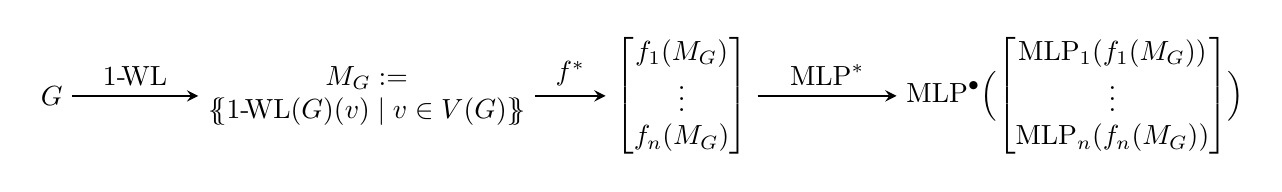
\begin{tikzpicture}
    \node (graph) at (0.0, 0.0) {$G$};
    \node[align=center] (multiset) at (4.0, 0.0) {$M_G :=$\\$\MSopen \wl(G)(v) \mid v \in V(G) \MSclose$};
    \node (encoding) at (8.0, 0.0) {$\begin{bmatrix}f_1(M_G)\\ \vdots \\f_n(M_G)\end{bmatrix}$};
    \node (mlp) at (13.0, 0.0) {$\text{MLP}^\bullet\Bigl( \begin{bmatrix}\text{MLP}_1 (f_1(M_G)) \\ \vdots \\\text{MLP}_n (f_n(M_G))\end{bmatrix} \Bigr)$};
    
    \draw[-stealth, thick] (graph.east) -- node [text width=2.5cm,midway,above,align=center ] {$\wl$} (multiset.west);
    \draw[-stealth, thick] (multiset.east) -- node [text width=2.5cm,midway,above,align=center ] {$f^*$} (encoding.west);
    \draw[-stealth, thick] (encoding.east) -- node [text width=2.5cm,midway,above,align=center ] {$\mlp^*$} (mlp.west);
    
\end{tikzpicture}
    \caption{The proof idea for \cref{lem:composition_lemma}, visualizing the functions $f^*$ and $\mlp^*$ and how they work when applied on an input $G \in \cX$. We denote here by $M_G$ the multiset of the colors of the nodes of $G$ after applying the $\wl$ algorithm.}
    \label{fig:proof_idea_parallelism}
\end{figure}


In the following two \cref{lem:encoding-indicator-func1,lem:encoding-indicator-func2}, we will show that the indicator function $\mathds{1}$ for the $\wliso$ relation on $\cX$ is \wlnn computable. We formally define this function for any pair of graphs $G_1, G_2 \in \cX$ as follows:
\begin{equation*}
    \mathds{1}_{G_1 \wliso G_2} = \begin{cases}
        1, \quad \text{if $G_1 \wliso G_2$}\\
        0, \quad \text{else}
    \end{cases}.
\end{equation*}
This function plays a crucial role in the proof of the theorem. We will first introduce an approximation of the inverse of this function in \cref{lem:encoding-indicator-func1} and then use this approximation for the proof of \cref{lem:encoding-indicator-func2} to construct a function $\varphi_{G_1}(G_2)$ that is equivalent to the indicator function $\mathds{1}_{G_1 \wliso G_2}$.

\begin{lemma}\label{lem:encoding-indicator-func1}
    Let $\cC$ be a collection of functions from $\cX$ to $\Rb$ computable by \wlnn that is \wldisc. Then for all $G^* \in \cX$, there exists a function $h_{G^*}$ from $\cX$ to $\Rb$ computable by \wlnn, such that on any input $G \in \cX: h_{G^*}(G) = 0$, if and only if, $G \wliso G^*$.
\end{lemma}

\begin{proof}
    Assume the above. Since $\cC$ is \wldisc, we know that for any pair of graphs $G_1, G_2 \in \cX$ with $G_1 \not\wliso G_2$, the function $h_{G_1, G_2} \in \cC$ exists, that distinguishes the pair, such that $h_{G_1, G_2}(G_1) \neq h_{G_1, G_2}(G_2)$. We define the function $\overline{h}_{G_1,G_2}$ working over $\cX$ for every such pair as follows:
    \begin{align}\label{eq:lemma_inidcator_function_1}
        \overline{h}_{G_1, G_2}(\cdot) &= |h_{G_1, G_2}(\cdot) - h_{G_1, G_2}(G_1)| \nonumber\\
        &= \max(h_{G_1, G_2}(\cdot) - h_{G_1, G_2}(G_1), \ 0) + \max(h_{G_1, G_2}(G_1) - h_{G_1, G_2}(\cdot), \ 0) \nonumber\\
        &= \text{ReLU}(h_{G_1, G_2}(\cdot) - h_{G_1, G_2}(G_1)) + \text{ReLU}(h_{G_1, G_2}(G_1) - h_{G_1, G_2}(\cdot))
    \end{align}
    Note, that in the equations above $h_{G_1, G_2}(G_1)$ is a fixed constant and the resulting function $\overline{h}_{G_1, G_2}$ is non-negative.
    Let $G_1 \in \cX$ now be fixed, then we will construct the function $h_{G_1}$ with the desired properties as follows:
    \begin{align}\label{eq:lemma_inidcator_function_2}
        h_{G_1}(\cdot) = \sum_{\substack{G_2 \in \cX \\ G_1 \not\wliso G_2}} \overline{h}_{G_1, G_2}(\cdot).
    \end{align}
    Since $\cX$ is finite, the sum is finite and therefore well-defined. Next, we will show that this construction fulfills the desired properties, by proving that for any input $G \in \cX: h_{G_1}(G) = 0$, if and only if, $G \wliso G_1$. Note that $G_1$ is arbitrary but fixed. Let $G \in \cX$ be an arbitrary input graph:
    \begin{enumerate}
        \item If $G_1 \wliso G$, then for every function $\overline{h}_{G_1, G_2}$ of the sum with $G_1 \not\wliso G_2$, we know, using \cref{lem:wl_relation_equivalence}, that $\overline{h}_{G_1, G_2}(G)$ is equal to $\overline{h}_{G_1, G_2}(G_1)$ which is by definition $0$, such that $h_{G_1}(G) = 0$.
        \item If $G_1 \not\wliso G$, then $\overline{h}_{G_1, G}(G)$ is a summand of the overall sum, and since $\overline{h}_{G_1, G}(G) > 0$, 
        we can conclude $h_{G_1}(G) > 0$ due to the non-negativity of each $\overline{h}_{G_1, G_2}$ function.
    \end{enumerate}
    Using \cref{lem:composition_lemma}, we can conclude that for any $G \in \cX$, $h_G$ is computable by \wlnn, as we can encode \cref{eq:lemma_inidcator_function_2} via a multilayer perceptron where the constant $h_{G_1, G_2}(G_1)$ of \cref{eq:lemma_inidcator_function_1} will be the bias of the corresponding channel, such that this \mlp exists.

    It is crucial to note that in the special case where no pair of graphs within $\cX$ is indistinguishable by the \wl isomorphism test from another, the function $h_{G_1}$ is still defined. However, it sums over zero summands, resulting in $h_{G_1}(\cdot) = 0$.
\end{proof}

Thus, we have proved that the function $h_{G}$ is \wlnn computable for any graph $G \in \cX$. The function $h_{G}$ approximates the inverted indicator function for the fixed graph $G$ by mapping graphs indistinguishable from $G$ by the \wl algorithm to $0$ while mapping every other graph to something strictly larger than $0$. The following proof will use this property to construct the indicator function.

\begin{lemma}\label{lem:encoding-indicator-func2}
    Let $\cC$ be a collection of functions from $\cX$ to $\Rb$ computable by \wlnn such that for all $G^* \in \cX$, there exists $h_{G^*} \in \cC$ satisfying $h_{G^*}(G) = 0 $, if and only if, $G \wliso G^*$, for all $G \in \cX$. Then for every $G^* \in \cX$, there exists a function $\varphi_{G^*} $ computable by \wlnn such that for all $G \in \cX$: $\varphi_{G^*}(G) = \mathds{1}_{G \wliso G^*}$.
\end{lemma}

\begin{proof}
    Assume the above. Due to $\cX$ being finite, we can define for every graph $G^*$ the constant:
    \begin{equation*}
        \delta_{G^*} \coloneqq \frac{1}{2} \min_{\substack{G \in \cX  \\  G \not\wliso G^*}} |h_{G^*}(G)|.
    \end{equation*}
    The constant $\delta_{G^*}$ represents the minimum value to which the corresponding function $h_{G^*}(\cdot)$ maps a graph $G$ that is distinguishable from $G^*$ by the \wl isomorphism test, multiplied by the factor $\frac{1}{2}$. The specific value of this factor is arbitrary; the crucial aspect is that it remains less than $1$, ensuring that the constant $\delta_{G^*}$ remains strictly smaller than the minimum value of $h_{G^*}(\cdot)$ for any graph $G$ where $G\not \wliso G^*$.

    It is important to note that in the special case where no pair of graphs within $\cX$ is indistinguishable by the \wl isomorphism test from another, the constant $\delta_{G^*}$ is not well-defined. For these cases, we can set $\delta_{G^*} := 1$ for all $G^* \in \cX$.

    We further introduce a so-called ``bump'' function $\psi_a(x)$ working from $\Rb$ to $\Rb$ paraemetrized by $a \in \Rb$ with $a > 0$ and defined as follows:
    \begin{align}\label{eq:lemma_encoding_indicator_func2}
        \psi_a(x) &\coloneqq \max(\frac{x}{a} -1,\ 0) + \max(\frac{x}{a}+1, \ 0) - 2 \cdot \max(\frac{x}{a}, \ 0) \nonumber\\
        &= \text{ReLU}(\frac{x}{a} -1) + \text{ReLU}(\frac{x}{a}+1) - 2 \cdot \text{ReLU}(\frac{x}{a})
    \end{align}
    The interesting property of $\psi_a$ is that it maps every value $x$ to $0$, except when $x$ is being drawn from the interval $(-a, a)$. In particular, it maps $x$ to $1$, if and only if, $x$ is equal to $0$. See \cref{fig:bump_function} for a plot of the relevant part of this function with exemplary values for $a$.

    We use these properties and the constant $\delta_{G^*}$ to define for every graph ${G^*} \in \cX$ the function $\varphi_{G^*}$ that is equivalent to the indicator function as follows:
    \begin{equation*}
        \varphi_{G^*}(\cdot) \coloneqq \psi_{\delta_{G^*}} (h_{G^*}(\cdot)).
    \end{equation*}
    We will prove the correctness of this construction by showing that for a fixed graph $G^*$ the following condition holds: $\forall G 
    \in \cX: \varphi_{G^*}(G) = 1$, if and only if, $G \wliso G^*$. For this lets consider two cases:
    \begin{enumerate}
        \item If $G \wliso G^*$, then $h_{G^*}(G) = 0$ resulting in $\varphi_{G^*}(G) = \psi_{\delta_{G^*}}(0) = 1$.
        \item If $G \not\wliso G^*$ then $h_{G^*}(G) \neq 0$, such that $|h_{G^*}(G)|> \delta_{G^*}$ so that $h_{G^*}(G) \not\in (-\delta_{G^*}, \delta_{G^*}) $ resulting in $\varphi_{G^*}(G) = 0$.
    \end{enumerate}
    Note that we can encode $\varphi_{G^*}$ using \cref{eq:lemma_encoding_indicator_func2} via a multilayer perceptron, where $\delta_{G^*}$ is a constant, such that this \mlp exists. With \cref{lem:composition_lemma} we can therefore conclude that $\varphi_{G^*}$ is computable by \wlnn for every graph ${G^*} \in \cX$.
\end{proof}

\begin{figure}[!htb]
    \centering
    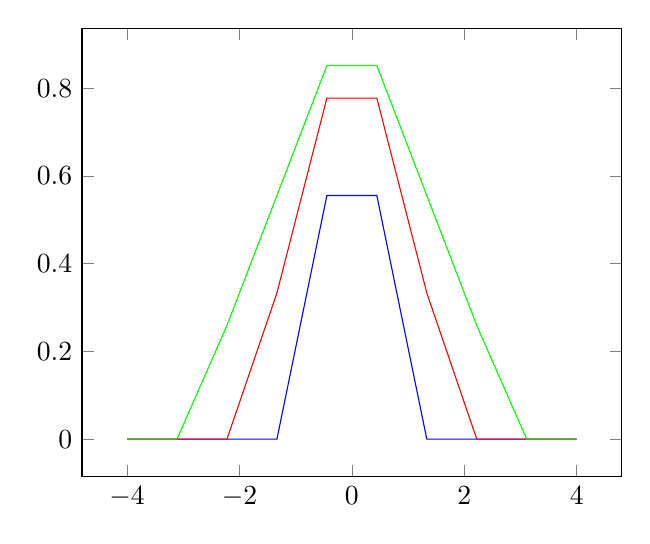
\begin{tikzpicture}
    \begin{axis}
    \addplot[domain=-4:4, samples=10, color=blue,]{max(x-1,0) + max(x+1,0) - 2*max(x,0)};
    \addplot[domain=-4:4, samples=10, color=red,]{max(x/2-1,0) + max(x/2+1,0) - 2*max(x/2,0)};
    \addplot[domain=-4:4, samples=10, color=green,]{max(x/3-1,0) + max(x/3+1,0) - 2*max(x/3,0)};
    \end{axis}
\end{tikzpicture}
    \caption{Illustration of the so-called ``bump'' function $\psi_a(x)$ used in the proof of \cref{lem:encoding-indicator-func2} with different exemplary values for $a$.}
    \label{fig:bump_function}
\end{figure}

We can now leverage all our lemmas to prove the overall theorem that any function $\cA$ computable by a \gnn can also be computed by \wlnn.
\begin{proof}[Proof of \cref{theorem:gnn_in_1wl}]\label{prof:gnn_in_1wl}
    Let $\cA$ be a function that works over $\cX$ to $\Rb$ computed by a \gnn model. We will prove that $\cA$ is \wlnn computable by decomposing the function and then argue that the decomposition is computable by a \wlnn model. For this let $G \in \cX$ be an arbitrary input graph, we can decompose $\cA(G)$ as follows:
    \begin{align}
        \cA(G) &= \Bigl( \ \frac{1}{|\cX/\!{\wliso}(G)|}\sum_{G^* \in \cX} \mathds{1}_{G \wliso G^*} \Bigr) \cdot \cA(G) \label{eq:gnn_decomposition1}\\
        &= \sum_{G^* \in \cX} \frac{1}{|\cX/\!{\wliso}(G)|} \cdot \cA(G) \cdot \mathds{1}_{G \wliso G^*} \label{eq:gnn_decomposition2}\\
        &= \sum_{G^* \in \cX} \frac{1}{|\cX/\!{\wliso}(G^*)|} \cdot \cA(G^*) \cdot \mathds{1}_{G \wliso G^*} \label{eq:gnn_decomposition3}\\
        &= \sum_{G^* \in \cX} \frac{\cA(G^*)}{|\cX/\!{\wliso}(G^*)|}  \cdot \varphi_{G^*}(G) \label{eq:gnn_decomposition4}
    \end{align}
    where $\cX/\!{\wliso}(G)$ denotes the set of all graphs that are equivalent to $G$ according to the $\wliso$ relation. We explain each equation step by step:
    \begin{itemize}[leftmargin=9em]
        \item[\cref*{eq:gnn_decomposition1}:] Multiplying $\cA(G)$ by the factor in the parentheses is correct because it is equal to $1$. This is because the sum ``counts'' the number of graphs $G^* \in \cX$ that are indistinguishable from the input graph $G$ by the \wl isomorphism test, and then the count is divided by the number of graphs in the equivalence class of $G$, which is the same as the count.
        \item[\cref*{eq:gnn_decomposition2}:] We can move both the factor $\cA(G)$ and $\frac{1}{|\cX/\!{\wliso}(G)|}$ into the sum by using the distributive property of the space $\Rb$.     
        \item[\cref*{eq:gnn_decomposition3}:] Due to the output of the indicator function $\mathds{1}$ being either $0$ or $1$, we can infer that the inner product of each summand can only be nonzero if $G^*$ is indistinguishable by the \wl isomorphism test from $G$. This implies that both are in the same equivalence class in these cases, such that $|\cX/\!{\wliso}(G)|$ is equal to $|\cX/\!{\wliso}(G^*)|$.\\
        Additionally, since \gnns are, at most, as good as the \wl algorithm in distinguishing pairs of non-isomorphic graphs (\cite{Morris2018,Xu2018}), we can use the fact that for every graph $G^* \in \cX$: if $G^* \wliso G$, then $\cA(G^*) = \cA(G)$. Using the same reasoning with the indicator function, we can replace the term $\cA(G)$ by $\cA(G^*)$.
        \item[\cref*{eq:gnn_decomposition4}:] Utilizing \cref{lem:encoding-indicator-func2}, we can replace the indicator function with $\varphi_{G^*}(G)$.
    \end{itemize}
    In conclusion, we have decomposed the \gnn function $\cA(G)$ such that the only factors that depend on the input graph $G$ are the functions $\varphi_{G^*}$, which take $G$ as input. This observation implies that all other factors are constants. Consequently, we can reason that the entire decomposition can be computed by a multilayer perceptron with a single layer, which takes the output of all $\varphi_{G^*}$ for all $G^* \in \cX$, applied to the input graph $G$. The multilayer perceptron then multiplies each of these values with the constant $\frac{\cA(G^*)}{|\cX/\!{\wliso}(G^*)|}$ and takes the sum. The existence of such a multilayer perceptron is evident, and when combined with \cref{lem:composition_lemma}, we can assert that this composition is \wlnn computable.

    Important to note, we can only do this since $\cX$ is finite, making the overall sum finite and the cardinality of $\cX/\!{\wliso}(G^*)$ well-defined for all graphs.
\end{proof}

\subsection{Proof of \cref*{theorem:1wl_in_gnn}: ``$\wlnn \subseteq \gnn$''}
In this section, we will prove the converse direction. Similar to the previous subsection, we will begin by introducing a set of lemmas that will play a crucial role in proving \cref{theorem:1wl_in_gnn}.

We start by showing the existence of a collection of functions computable by \gnns that is \wldisc. For the proof, we will devise message-passing layers for a \gnn that effectively compute a single iteration of the \wl algorithm per layer. Afterward, we show that with a proper choice of the \textsf{Readout} function, we construct a collection of \gnn functions that is \wldisc. 
Although prior works by \cite{Morris2018} and \cite{Xu2018} have already demonstrated how to construct message-passing layers to compute a single iteration of the \wl algorithm per layer, we include our own construction with our notation in the proof for two crucial reasons. Firstly, it ensures the completeness of our proof without assuming major parts. Secondly, and most importantly, it effectively highlights the remarkable similarities and key distinctions between the \wl algorithm and \gnns in general.
\begin{lemma}[GNN \wldisc]\label{lem:gnn_1wl_disc}
    There exists a collection $\cC$ of functions from $\cX$ to $\Rb$ computable by \gnns that is \wldisc.
\end{lemma}

\begin{proof}
    Due to $\cX$ being finite, we define the constants $n, m, k$ as follows:
    \begin{equation*}
        n := \max_{G \in \cX} |V(G)|, \quad  m := \sum_{G \in \cX} |V(G)|, \quad\text{and}\quad k := 1 + \max_{\substack{G \in \cX \\ v \in V(G)}} |l_G(v)|,
    \end{equation*}
    such that $n$ is the maximum number of nodes of any graph in $\cX$, $m$ is the total number of nodes of the set $\cX$, and $k$ is the largest label of any node of a graph in $\cX$ plus $1$.

    We will utilize these constants to construct the collection of functions $\cC := \{ \cA_c \mid c \in \Nb \}$ that is \wldisc. For the remainder of this proof, we first describe the construction of an arbitrary $\cA_c \in \cC$ and afterward, prove that the collection $\cC$ is \wldisc.

    Each $\cA_c$ consists of $n$ message-passing layers. We define the input layer $f^{(0)}(v) \coloneqq v$ as the identity functions such that there is no preprocessing of the node labels. Further, we define every other layer $t$ with $1 \leq t \leq n$ as follows:
    \begin{align*}
        f^{(t)}(v) \coloneqq f^{(t)}_{\text{merge}}(f^{(t-1)}(v), \ \MSopen f^{(t-1)}(u) \mid u \in \cN(v)\MSclose).
    \end{align*}
    Here $f^{(t)}_{\text{merge}}$ is an injective function that maps its input into its codomain:
    \begin{equation*}
       \{ i \in \Nb \mid k + (t-1) \cdot m \ \leq \  i \ \leq \ k + t \cdot m \}
    \end{equation*}
    This function exists due to the finiteness of $\cX$. We can upper bound the cardinality of its domain, the number of unique tuples, by the total number of nodes in $\cX$, which is $m$, and since the cardinality of its codomain is exactly $m$, we can conclude the existence of the function.

    Next, we will define the \textsf{Readout} function of $\cA_c$ to be the function that returns the number of nodes colored as $c$ in the coloring of $f^{(n)}$.
    
    By leveraging the results of \textit{theorem 3} from the work of \cite{Xu2018}, we can infer that each layer of each $\cA_c$ computes a single iteration of the \wl algorithm. This observation makes sense as the update equation for each layer injectively maps each tuple to a previously unused color, similar to how the \textsf{Relabel} function of the \wl algorithm works. Moreover, since the \wl algorithm terminates on any graph $G \in \cX$ after at most $|V(G)| \leq n$ iterations, the coloring computed by the layers of each $\cA_c$ effectively performs $n$ iterations of the \wl algorithm when applied to any graph $G \in \cX$. Due to the convergence behavior of the \wl algorithm, these additional iterations do not increase the expressiveness of the colorings computed by each $\cA_c$, such we can conclude for any graph $G \in \cX$:
    \begin{equation*}
       \forall c \in \Nb: |\{ v \in V(G) \mid  f^{(n)}(v) = c \}| = |\{ v \in V(G) \mid  \wl(G)(v) = c \}|,
    \end{equation*}
    which states that the colorings are equal for a bijection $\phi : \Nb \rightarrow \Nb$, such that we can infer that they are equally expressive for distinguishing non-isomorphism.

    To prove that the collection $\cC$ is \wldisc, we need to show two properties: 1) Each function in the collection is permutation invariant, and 2) For each pair of graphs in $\cX$ distinguishable by the \wl isomorphism test, there must exist a function in the collection that also distinguishes the pair.
   
    For the first property, by \cref{def:gnn} of \gnns, all functions computed by \gnns are permutation-invariant.
    Regarding the second property, consider $G_1, G_2 \in \cX$ with $G_1 \not\wliso G_2$. Let $C_1$ and $C_2$ represent the final colorings computed by the $\wl$ algorithm when applied to $G_1$ and $G_2$, respectively. Since $G_1 \not\wliso G_2$, there exists a color $c \in \Nb$ such that $\hist_{G_1,C_1}(c) \neq \hist_{G_2,C_2}(c)$. Since, we know that each $\cA_c$ computes equally expressive colorings of $G_1$ and $G_2$, we know that there exists a $c' \in \Nb$, such that $\cA_{c'}(G_1) \neq \cA_{c'}(G_2)$.
\end{proof}
 
Similar to the proof in the previous subsection, we will use \cref{lem:composition_lemma_gnn} to introduce the ability to construct \gnns that take in as input multiple \gnns and then apply a multilayer perceptron to the combined output. This insight is leveraged in the following two corollaries in the proof, as well as in the final proof.

\begin{lemma}[\gnn Composition]\label{lem:composition_lemma_gnn}
    Let $\cC$ be a collection of functions computable by \gnns. Further, let  $\cA_1, \dots , \cA_n \in \cC$ and $\mlp^\bullet$ a suitable multilayer perceptron, then the function $\hat{\cA}(\cdot) \coloneqq \mlp(\cA_1(\cdot), \dots, \cA_n(\cdot))$ is also computable by a \gnn.
\end{lemma}

\begin{proof}
    Before we begin the proof, we briefly introduce two notations. For any $x \in \Rb^d$, we will use the notation $x[i]$ to indicate the $i$.th element of the vector $x$. Additionally, we indicate the merge and aggregation function used in layer $t$ by $\cA_i$ as $f^{(t)}_{\text{merge}, i}$ and $f^{(t)}_{\text{agg}, i}$. Similarly, we denote the \textsf{Readout} function as $\textsf{Readout}_i$ and the input function of $\cA_i$ as $f^{(0)}_i$.
    
    We will prove the lemma by giving a construction of a \gnn model computing $\hat{\cA}$. For the ease of readability and to reduce the complexity of the subsequent construction, we assume that for all $\cA_i$ its functions $f^{(t)}_{\text{merge}, i}, f^{(t)}_{\text{agg}, i}$ and $\textsf{Readout}_i$ map into the one-dimensional space $\Rb$ for all layers $t$. With this assumption, we avoid the need for a formal notation of the number of dimensions each of these functions map to.

    Let $T$ be the maximum number of layers of all $\cA_1, \dots, \cA_n$. We construct the \gnn $\hat{\cA}$ with $T$ layers, with the input layer working as follows on an input graph $G$:
    \begin{align*}
        \forall v \in V(G): \ \hat{f}^{(0)}(v) \coloneqq \begin{bmatrix}
            f^{(0)}_1(v)\\
            \vdots\\
            f^{(0)}_n(v)
        \end{bmatrix},
    \end{align*}
    and each other layer $0 < t \leq T$ utilizing the merge $\hat{f}^{(t)}_{\text{merge}}$ and aggregation $\hat{f}^{(t)}_{\text{agg}}$ functions as constructed in the following:
    \begin{align*}
        \hat{f}^{(t)}_{\text{merge}} (\hat{f}^{(t-1)}(v), \ Agg) &:= \begin{bmatrix}
            f^{(t)}_{\text{merge}, 1}(\hat{f}^{(t-1)}(v)[1],\ Agg[1])\\
            \vdots\\
            f^{(t)}_{\text{merge}, n}(\hat{f}^{(t-1)}(v)[n],\ Agg[n])
        \end{bmatrix},\quad \text{and}\\
        \hat{f}^{(t)}_{\text{agg}}(\MSopen \hat{f}^{(t-1)}(w) \mid w \in \mathcal{N}(v) \MSclose ) &:= \begin{bmatrix}
            f^{(t)}_{\text{agg}, 1}(\MSopen \hat{f}^{(t-1)}(w)[1] \mid w \in \mathcal{N}(v) \MSclose)\\
            \vdots\\
            f^{(t)}_{\text{agg}, n}(\MSopen \hat{f}^{(t-1)}(w)[n] \mid w \in \mathcal{N}(v) \MSclose)
        \end{bmatrix}.
    \end{align*}
    Note that, not all $\cA_i$ will be comprised of $T$ layers, such that for these cases the functions $f^{(t)}_{\text{merge}, i}$ and $f^{(t)}_{\text{agg}, i}$ will not be defined for all $t \in [T]$. In these cases, we define the functions as follows:
    \begin{align*}
        f^{(t)}_{\text{merge}, i}(\hat{f}^{(t-1)}(v), \ Agg) &\coloneqq \hat{f}^{(t-1)}(v), \quad \text{and}\\
        f^{(t)}_{\text{agg}, i}(\MSopen \hat{f}^{(t-1)}(w) \mid w \in \mathcal{N}(v) \MSclose) &\coloneqq 0.
    \end{align*}
    This definition of $f^{(t)}_{\text{merge}, i}$ and $f^{(t)}_{\text{agg}, i}$ results in the fact that the representation computed in the last layer of $\cA_i$ is forwarded to the last layer $T$ of $\hat{\cA}$. Finally, we construct the \textsf{Readout} function of $\hat{\cA}$ as follows:
    \begin{align*}
        \textsf{Readout}(\MSopen \hat{f}^{(T)}(v) \mid v \in V(G) \MSclose) \coloneqq \mlp^\bullet \circ \begin{bmatrix}
            \textsf{Readout}_1(\MSopen \hat{f}^{(T)}(v)[1] \mid v \in V(G) \MSclose)\\
            \vdots\\
            \textsf{Readout}_n(\MSopen \hat{f}^{(T)}(v)[n] \mid v \in V(G) \MSclose)
        \end{bmatrix}.
    \end{align*}
    With this, the proof concludes. Note that this proof can easily be extended to work without the assumption of each function mapping into a one-dimensional space.
\end{proof}

As a consequence of the previous two lemmas, we find ourselves in a similar position as at the beginning of the proof in \cref{sec:proof_theorem:1wl_in_gnn}. Specifically, we have established, through \cref{lem:gnn_1wl_disc}, the existence of a collection $C$ of functions that can be computed by \gnns and can effectively distinguish any pair of graphs that are also distinguishable by the \wl algorithm. Furthermore, with \cref{lem:composition_lemma_gnn}, we have demonstrated that the composition of multiple \gnns and a multilayer perceptron remains computable by a single \gnn. Consequently, we can use the same proofs of \cref{lem:encoding-indicator-func1,lem:encoding-indicator-func2} to derive the \cref{lem:encoding-indicator-func1_gnn,lem:encoding-indicator-func2_gnn}. 

\begin{corollary}\label{lem:encoding-indicator-func1_gnn}
    Let $\cC$ be a collection of functions from $\cX$ to $\Rb$ computable by \gnns that is \wldisc. Then for all $G^* \in \cX$, there exists a function $h_{G^*}$ from $\cX$ to $\Rb$ computable by \gnn, such that on any input $G \in \cX: h_{G^*}(G) = 0$, if and only if, $G \wliso G^*$.
\end{corollary}
\begin{corollary}\label{lem:encoding-indicator-func2_gnn}
    Let $\cC$ be a collection of functions from $\cX$ to $\Rb$ computable by \gnns such that for all $G^* \in \cX$, there exists $h_{G^*} \in \cC$ satisfying $h_{G^*}(G) = 0 $, if and only if, $G \wliso G^*$, for all $G \in \cX$. Then for every $G^* \in \cX$, there exists a function $\varphi_{G^*} $ computable by \gnns such that for all $G \in \cX$: $\varphi_{G^*}(G) = \mathds{1}_{G \wliso G^*}$.
\end{corollary}

In conclusion, the corollaries establish the computability of the indicator function $\mathds{1}_{G_1 \wliso G_2}$ over the set $\cX$ by a \gnn. Building upon these results, we can now utilize all our lemmas to prove the theorem, which states that any function $\cB$ computable by a \wlnn can also be computed by a \gnn.

\begin{proof}[Proof of \cref*{theorem:1wl_in_gnn}]
    Let $\cB$ be a function that works over $\cX$ to $\Rb$ computed by a \wlnn model. We will prove that $\cB$ is \gnn computable by decomposing the function and then argue that the decomposition is computable by a \gnn model. For this let $G \in \cX$ be an arbitrary input graph, we can decompose $\cB(G)$ as follows:
    \begin{align}
        \cB(G) &= \Bigl( \ \frac{1}{|\cX/\!{\wliso}(G)|}\sum_{G^* \in \cX} \mathds{1}_{G \wliso G^*} \Bigr) \cdot \cB(G) \nonumber\\
        &= \sum_{G^* \in \cX} \frac{1}{|\cX/\!{\wliso}(G)|} \cdot \cB(G) \cdot \mathds{1}_{G \wliso G^*} \nonumber\\
        &= \sum_{G^* \in \cX} \frac{1}{|\cX/\!{\wliso}(G^*)|} \cdot \cB(G^*) \cdot \mathds{1}_{G \wliso G^*} \label{eq:wlnn_decomposition3}\\
        &= \sum_{G^* \in \cX} \frac{\cB(G^*)}{|\cX/\!{\wliso}(G^*)|}  \cdot \varphi_{G^*}(G) \label{eq:wlnn_decomposition4}
    \end{align}
    where $\cX/\!{\wliso}(G)$ denotes the set of all graphs that are equivalent to $G$ according to the $\wliso$ relation. Since the decomposition is very similar to the one present in the proof of \cref{theorem:gnn_in_1wl}, we will only provide reasoning for the correctness of \cref{eq:wlnn_decomposition3,eq:wlnn_decomposition4}. For all other equations, refer to the explanation provided in the proof of \cref{theorem:gnn_in_1wl}
    \begin{itemize}[leftmargin=9em]
        \item[\cref*{eq:wlnn_decomposition3}:] Due to the output of the indicator function $\mathds{1}$ being either $0$ or $1$, we can infer that the inner product of each summand can only be nonzero if $G^*$ is indistinguishable by the \wl isomorphism test from $G$. Using \cref{lem:wl_relation_equivalence}, we know that for every graph $G^* \in \cX$: if $G^* \wliso G$, then $\cB(G^*) = \cB(G)$.
        \item[\cref*{eq:wlnn_decomposition4}:] Utilizing \cref{lem:encoding-indicator-func2_gnn}, we can replace the indicator function with $\varphi_{G^*}(G)$.
    \end{itemize}
    In conclusion, we have decomposed the \gnn function $\cB(G)$ such that the only factors that depend on the input graph $G$ are the functions $\varphi_{G^*}$, which take $G$ as input. This observation implies that all other factors are constants. Consequently, we can reason that the entire decomposition can be computed by a multilayer perceptron with a single layer, which takes the output of all $\varphi_{G^*}$ for all $G^* \in \cX$, applied to the input graph $G$. The multilayer perceptron then multiplies each of these values with the constant $\frac{\cB(G^*)}{|\cX/\!{\wliso}(G^*)|}$ and takes the sum. The existence of such a multilayer perceptron is evident, and when combined with \cref{lem:composition_lemma}, we can assert that this composition is \wlnn computable.

    Important to note, we can only do this since $\cX$ is finite, making the overall sum finite and the cardinality of $\cX/\!{\wliso}(G^*)$ well-defined for all graphs.
\end{proof}
The empirical part is divided into blbnalanb

\section{Testing Configuration}
This section delves into the configuration and setup of our empirical testing. We begin by presenting our carefully selected datasets, which serve as the foundation for our evaluation. We highlight specific insights and characteristics of these datasets that make them compelling choices for our study. Afterward, we focus on the models we employ for testing and subsequent result comparison. We provide a comprehensive overview of the selected models, outlining their key features and motivations behind their inclusion in our evaluation. Subsequently, we provide a detailed description of the training pipeline and explain specific hyperparameters for which we will optimize these models.

\subsection{Datasets}
We will first explain our choice of datasets and introduce each dataset individually. Afterward, we will explore essential observations that are to be considered when assessing the actual empirical results.

\subsubsection{Choice of Datasets}
In selecting the datasets for our thesis, we adhered to two fundamental principles to ensure the robustness and diversity of our evaluation for \gnn and \wlnn models. The first principle focuses on using widely recognized benchmark datasets that have been extensively employed in previous studies. This principle enables us and readers to make meaningful comparisons with existing results. The second principle focuses on choosing datasets that are distinct from one another in terms of both their application domains and the way they encode information in graphs.

To fulfill the first principle, we opted for datasets from the TUDataset library. This library, curated by \cite{Mor+2020}, serves as a widely recognized standard for evaluating graph-related methods.

Regarding the second principle, we incorporated the insights from \cite{Liu2022}, who developed a comprehensive taxonomy of common graph benchmark datasets. Their work examined the degree to which information is encoded in graph structures compared to node features with respect to solving the task of the datasets. Based on their taxonomy, they categorized datasets into three distinct classes:
\begin{enumerate}
	\item Datasets in which the most crucial information for solving the task is contained in the node features.
	\item Datasets similar to the first category, but with the significant exception that the node degree strongly correlates with the node features. In these datasets, utilizing simple structural information, such as computing the node degree, is as beneficial for solving the task as using the original node features.
	\item Datasets where the most crucial information is encoded within the graph structure itself.
\end{enumerate}
These categories help us understand how information is encoded in various datasets, such that we aim to choose datasets from all three categories.

As a result of considering these two principles, we selected the following datasets for our thesis: \textsc{Enzymes}, \textsc{Imdb-Binary}, \textsc{Mutag}, \textsc{Nci1}, \textsc{Proteins}, and \textsc{Reddit-Binary} for classification tasks, and \textsc{Alchemy} and \textsc{Zinc} for regression tasks. For an overview of the elemental properties of each dataset, see \cref{tab:overview_datasets}. We will now shortly introduce each dataset individually: \newline

\textsc{Enzymes}, provided by \cite{Borgwardt2005}, is a dataset consisting of proteins in their tertiary structure, categorized into six distinct enzyme classes. Each node represents a secondary structure, and has an edge to its three spatially closest nodes. Furthermore, each node feature encodes the type of secondary structure (\textit{helix}, \textit{sheet} or \textit{turn}), as well as physical and chemical information. \newline


\textsc{Imdb-Binary}, provided by \cite{Yanardag2015}, is a dataset comprising ego networks. Each node in the network represents an actor/actress, and a unidirectional edge exists between two nodes if and only if the corresponding actors played together in a movie. The task involves determining whether each ego network's genre is \textit{action} or \textit{romance}. \newline

\textsc{Mutag}, provided by \cite{Debnath1991}, is a dataset comprising Nitroaromatic compounds. Each compound is represented by a graph in which nodes represent atoms, with their types encoded as node features, and edges represent atomic bonds. The task involves determining whether a given compound has a mutagenic effect on Salmonella typhimurium bacteria. \newline

\textsc{Nci1}, provided by \cite{Wale2008}, comprises graph representations of chemical compounds. In these graphs, nodes represent atoms, and edges represent atomic bonds. Moreover, the atom types are encoded in the node features. The overall task involves determining whether a given compound is active or inactive in inhibiting non-small cell lung cancer.\newline

\textsc{Proteins}, provided by \cite{Borgwardt2005}, contains proteins encoded similarly to ENZYMES. The task here is to determine whether each graph represents an enzyme. \newline

\textsc{Reddit-Binary}, provided by \cite{Yanardag2015}, involves graphs that are derived from popular Reddit communities. The nodes in these graphs represent users who are active in the community, while the edges represent interactions between the users. The task is to identify whether a graph belongs to a community that is focused on questions and answers, or one that is focused on discussions. \newline

\textsc{Alchemy}, provided by \cite{Chen2019alchemy}, consists of organic molecules, with each node representing an atom and each edge representing an atomic bond. Additionally, each node feature encodes various properties for each atom, while each edge encodes the bond type and distance between atoms. The overall task is to compute 12 different continuous quantum mechanical properties for each graph. \newline

\textsc{Zinc}, provided by \cite{Bresson2019} and \cite{Irwin2012}, consists of molecular graphs where each node represents a heavy atom, and the corresponding node feature specifies its type. The edges in the graph encode the bonds between atoms, and their features further describe the type of bond. The task is to calculate a molecular property known as constrained solubility ($\log P - \text{SA} - \text{cycle}$).\newline

\begin{table}[]
	\begin{center}
		\caption{Dataset statistics and properties for graph-level prediction tasks. This table has been adapted from \cite{Morris2022}.}
		\resizebox{0.975\textwidth}{!}{ 	\renewcommand{\arraystretch}{1.05}
			\begin{tabular}{@{}c <{\enspace}@{}lccccccc@{}}\toprule
				& \multirow{3}{*}{\vspace*{4pt}\textbf{Dataset}} & \multicolumn{7}{c}{\textbf{Properties}}\\
				\cmidrule{3-9}
				                         & & \shortstack{Number\\of graphs} & \shortstack{Number of\\classes/targets} & \shortstack{$\varnothing$ Number\\of nodes} & \shortstack{$\varnothing$ Number\\ of edges} & \shortstack{Node\\labels} & \shortstack{Edge\\labels} & \shortstack{Taxonomy \\Category} \\ \midrule
				\multirow{6}{*}{\rotatebox{90}{Classification}}
				& $\textsc{Enzymes}$       & 600               & 6                         & 32.6                          & 62.1                          & \cmark                   & \xmark  & 1    \\
				& $\textsc{IMDB-Binary}$   & 1\,000            & 2                         & 19.8                          & 96.5                          & \xmark                   & \xmark   & 3   \\
				& $\textsc{Mutag}$         & 188               & 2                         & 17.9                          & 19.8                          & \cmark                   & \xmark   & 2   \\
								
				& $\textsc{NCI1}$          & 4\,110            & 2                         & 29.9                          & 32.3                          & \cmark                   & \xmark   & 3   \\
				& $\textsc{Proteins}$      & 1\,113            & 2                         & 39.1                          & 72.8                          & \cmark                   & \xmark  & 2    \\
				& $\textsc{Reddit-Binary}$ & 2\,000            & 2                         & 429.6                         & 497.8                         & \xmark                   & \xmark & 3     \\ 
				\midrule
				\multirow{2}{*}{\rotatebox{90}{Reg.}}
				& $\textsc{Alchemy}$       & 202\,579          & 12                        & 10.1                          & 10.4                         & \cmark                   & \cmark & -     \\
				& $\textsc{Zinc}$       & 249\,456          & 1                        & 23.1                         & 24.9                          & \cmark                   & \cmark & -     \\
				\bottomrule
			\end{tabular}}
		\label{tab:overview_datasets}
	\end{center}
\end{table}

\subsubsection{Analysis of the Datasets}
To ensure the reliability and fairness of our evaluation, one of our initial steps was to assess the balance of our selected datasets for classification. We employed the normalized Shannon index to evaluate the balance of a dataset, where a value close to $0$ indicates maximum imbalance, while a value close to $1$ signifies perfect balance. See \cref{sec:definition_shannon_index} in the Appendix for a formal definition of this metric.

\begin{table}[H]
	\caption{An overview of the normalized Shannon index calculated for each dataset.}
	\label{tab:shannon_index}
	\centering
    \resizebox{.975\textwidth}{!}{ 	\renewcommand{\arraystretch}{0.9}
		\begin{tabular}{@{}c <{\enspace}@{}lcccccc@{}}	\toprule
			& \multirow{3}{*}{\vspace*{4pt}}&\multicolumn{6}{c}{\textbf{Dataset}}\\\cmidrule{3-8}
			& & {\textsc{Enzymes}}          & {\textsc{Imdb-Multi}}  & {\textsc{Mutag}}           & {\textsc{NCI1}}       & {\textsc{Proteins}}  & {\textsc{Reddit-Binary}}
			\\
			\toprule
			\multirow{1}{*}{} 	&
			Shannon index & 1 & 1 & 0.920 & 1 & 0.973 & 1 \\
			\bottomrule
		\end{tabular}}              
\end{table}

\Cref{tab:shannon_index} provides an overview of the normalized Shannon index computed for each selected classification dataset. Upon analyzing the data, we observed that all the datasets exhibit high balance, as all their values are close to $1$. This finding assures us that the datasets do not suffer significant class imbalances, which will remain important in the following section.

In addition to the balance of all datasets, another important aspect is understanding the upper bound of performance achievable by both \gnn and \wlnn models on these datasets. Unlike in other areas of machine learning where multilayer perceptron models can achieve near-perfect performance due to their universal approximation capabilities (\cite{Hornik1991}), \gnn and \wlnn models have inherent limitations on their expressiveness. This restriction stems from the fact that the expressiveness of the \wl algorithm limits the performance of both frameworks. In detail, if the \wl algorithm can not distinguish a pair of graphs in a dataset, then neither a \gnn nor a \wlnn model can.

While we have pointed out that the \wl algorithm is, in general, quite powerful in distinguishing pairs of graphs in \cref{sec:related_work}; we also explained that it is not complete. Therefore, assuming that \gnn or \wlnn models exist that can achieve almost perfect accuracy on all classification datasets is not reasonable. Thus, we calculated the theoretical maximum accuracy achievable by the perfect model for each dataset. In detail, we even investigated how many iterations of the \wl algorithm it takes to achieve this accuracy. For a comprehensive overview of the accuracies achievable on all datasets, please refer to \cref{tab:max_accuracies}. In this table, we have included the accuracy achievable when running the \wl algorithm for $0$ iterations, which essentially means taking the initial node features as the coloring for iteration $0$ and assessing the expressiveness of this initial coloring.

\begin{table}[H]
	\caption{An overview of the maximum theoretical classification accuracy achievable for each dataset based on the number of \wl iterations in percent. A hyphen ``-'' indicates that the maximum accuracy has converged with fewer iterations, implying that further iterations do not improve the accuracy.}
	\label{tab:max_accuracies}
    \resizebox{.975\textwidth}{!}{ 	\renewcommand{\arraystretch}{0.9}
		\begin{tabular}{@{}c <{\enspace}@{}lcccccc@{}}	\toprule
			& \multirow{3}{*}{\vspace*{4pt}\textbf{1-WL}}&\multicolumn{6}{c}{\textbf{Dataset}}\\\cmidrule{3-8}
			& & {\textsc{Enzymes}}         &  {\textsc{Imdb-Binary}}  & {\textsc{Mutag}}           & {\textsc{NCI1}}       & {\textsc{Proteins}}  & {\textsc{Reddit-Binary}}
			\\
			\toprule
			\multirow{6}{*}{} 	&
			Iterations: $0$       &  81.4 & 60.6 & 93.1 & 91.3 & 91.9 & 83.9
			\\ 
			& Iterations: $1$    & 100.0 & 88.6 & 95.7 & 99.5 & 99.7 & 100.0
			\\
			& Iterations: $2$    & - & - & 99.5 & 99.8 & - & - 
			\\
			& Iterations: $3$   & - & - & 100.0 & 99.8 & - & - 
			\\
			& Iterations: $4$    & - & - & - & - & - & -
			\\
			\cmidrule{2-8}\morecmidrules\cmidrule{2-8}
			& Max Accuracy     & 100.0 & 88.6 & 100.0 & 99.8 & 99.7 & 100.0      
			\\
			\bottomrule
		\end{tabular}}              
\end{table}

Upon examining the results, we observe that all datasets exhibit perfect or near-perfect theoretical classification accuracies. This result makes interpreting results obtained from actual \wlnn or \gnn models later on more straightforward. Additionally, the accuracy achievable after each number of iterations provides a theoretical lower limit on the number of message-passing layers a \gnn must be composed of to be even capable of achieving this accuracy. 

We have conducted the same analyzes on additional datasets, as their results might be valuable to the reader. For these, see \cref{tab:max_accuracies_app} in the Appendix.


\subsection{Choice of Models}
In selecting our models, we aimed to use techniques that are relatively generic and not highly specialized for any of the datasets, such that insights we gain upon analyzing the model's performance can be generalized better. Consequently, we opted for a basic set of models to maintain simplicity and versatility.

\subsubsection{\wlnn Models}
Our primary consideration for the \wlnn models revolves around choosing an encoding function, as all other components are fixed. To keep things straightforward, we decided to employ encoding functions consisting of two main components. Firstly, an optional preprocessing step that operates on the colors computed by the \wl algorithm. Secondly, a basic pooling function for transforming the color histogram into a fixed-size vector.

In more detail, the optional preprocessing step involves a simple look-up table. If utilized, this step maps each color injectively to a vector in the range of $[-1, 1]^n$, where the value of $n$ is a hyperparameter. By encoding the color information into higher dimensions, this approach aims to enhance efficiency during subsequent processing steps. For the second step, the pooling component, we selected elementary functions such as elementwise \textsf{Max}, \textsf{Mean}, and Summation (\textsf{Sum}). In summary, each of the \wlnn models can be uniquely identified by their encoding functions; therefore, we will refer to each model by their encoding function as follows:
\begin{equation*}
	\text{Embedding}-\{\textsf{Max}, \textsf{Mean}, \textsf{Sum}\} \quad \text{or} \quad \{\textsf{Max}, \textsf{Mean}, \textsf{Sum}\},
\end{equation*}
where ``Embedding'' indicates the use of the optional preprocessing step.

\subsubsection{\gnn Models}
As mentioned in the introduction to this section, our focus is on keeping the models basic. Hence, we opted for \gin by \cite{Xu2018}, \gcn by \cite{Kip+2017}, and \gat by \cite{Velivckovic2017} as the base architecture for the message-passing layers. Each of these architectures was chosen for specific reasons.

Firstly, we included \gin as an obvious candidate because it has been proven to be as expressive as the 1-WL algorithm. This characteristic makes it interesting when comparing it to \wlnn models.
Next, we also included \gcn based on its good empirical success in recent years. Furthermore, the insights provided by \cite{Nikolentzos2023} demonstrated that, in a certain sense, the node features computed by \gcn and \gin are similar, making \gcn a reasonable alternative to \gin in cases where the advantage of \gin's expressiveness is not needed.
Lastly, we added \gat as an alternative approach to the other two architectures. In detail, \cite{Nikolentzos2023} also showed that the node features computed by \gat are entirely different from those computed by \gin or \gcn.

Regarding the choice of \textsf{Readout} functions, we decided to utilize functions that are composed of two components. The first component is one of the elementwise pooling functions, such as \textsf{Max}, \textsf{Mean}, and \textsf{Sum}, to aggregate the information from a graph representation into a fixed-sized vector. Secondly, we incorporate a multilayer perceptron to process the aggregated information further, similarly to the \wlnn models.

In summary, each of the \gnn models can be uniquely identified by their \gnn architecture and the pooling function utilized; therefore, we will refer to each model by these two properties as follows:
\begin{equation*}
	{\{\gat, \gcn, \gin\}} - \{\textsf{Max}, \textsf{Mean}, \textsf{Sum}\}.
\end{equation*}

Note that the selection of the Readout function creates similarities between the \gnn and \wlnn models. These similarities play a crucial role in ensuring that any empirical differences observed between the two frameworks are not attributed to the utilization of more powerful techniques.

\subsection{Experimental Setup}

For the empirical testing, we took measures to ensure the reliability of our results in terms of hyperparameter configuration. Additionally, we aimed to ensure the reproducibility of the training pipeline for each model.

\subsubsection{Testing Procedure}

We started by conducting tests on the classification datasets, which serve as the basis for our evaluation. In our testing code, we employ a 10-fold cross-validation approach. Within this framework, we further partitioned the training data randomly, allocating 10\% of it for validation purposes. Consequently, each training iteration consisted of 0.81\% of the original dataset as the training set, 9\% as the validation set, and 10\% as the test set. We repeat this testing procedure five times to mitigate the influence of randomness on the model's performance. Ultimately, we recorded the mean accuracy on the test set along with its standard deviation as the primary performance metric of the model. Note that the use of standard cross-validation for generating the splits and the choice of mean accuracy as our primary metric is reasonable and justified as the datasets are highly balanced, as demonstrated in Section 2.

In the case of the regression datasets, we adopted a slightly different testing procedure. Due to their larger scale compared to the classification datasets, we opted for a more time-efficient approach. To achieve this, we utilized pre-existing training pipelines developed in \cite{Mor+2020} and \cite{Morris2022speqnets}. These pipelines use a fixed training, validation, and test split, accelerating the testing process. Similar to the classification datasets, we performed five runs for each model configuration and conducted a hyperparameter sweep for all model configurations. We record the mean absolute error and its standard deviation, as well as the mean logarithmic absolute error and its standard deviation across all runs. Furthermore, we test two splits for each regression dataset: one utilizing only 10,000 samples for training, while the other split uses the entire training set.

\subsubsection{Hyperparameter Optimization}\label{sec:hyperparam}
To ensure the comparability of our results with other works and limit the number of hyperparameters requiring optimization, we followed standard practices when configuring our models. Detailed information on all hyperparameters, including the ones we optimized, can be found in \cref{tab:sweep_wlnn} for the \wlnn models used in classification tasks, \cref{tab:sweep_gnn} for the \gnn models employed in classification tasks, and \cref{tab:sweep_wlnn_reg} for the \wlnn models utilized in the regression task in the Appendix. We will shortly discuss the most critical parameters we optimized for:

Early in our investigations, we made a significant observation regarding the learning performance of \wlnn models. We noticed considerable performance discrepancies when comparing \wlnn models using the standard version of the \wl algorithm with the one from GNNs. Consequently, we investigated the possibility of parametrizing the \wl algorithm to enhance control over the expressiveness of the colorings it computes. Specifically, we focused on two crucial parameters: 1) the number of iterations and 2) the usage of its convergence behavior as an early termination criterion.

The advantage of this more granular parametrization is that it enables us to apply the same number of \wl iterations to each graph processed by a \wlnn model by deactivating the convergence behavior and fixing the number of iterations. By deactivating this behavior and keeping the number of iterations minimal, we observed that the number of colors used by the \wl algorithm remained contained. As a result, the \mlp component of each \wlnn model seems to generalize better, significantly improving performance. Therefore, one of the most crucial hyperparameters we optimized for all \wlnn models was the number of \wl iterations. Additionally, if employed, the size of the dimension of the look-up table was another significant parameter to optimize.

In contrast, the hyperparameter selection for the \gnn models was relatively less intricate. The key parameters of interest here are the number of message-passing layers and the size of the hidden dimensions used in each layer. The reason for this is that the number of layers directly corresponds to the expressiveness of the GNN, as demonstrated in the proof, while the size of the hidden dimensions enables easier learning by allowing the model to store more information during graph processing.

\subsubsection{Implementation Details and Result Accessibility}
The implementation of our models and training procedures was carried out using \textsc{Python 3.10} along with the open-source library \textsc{PyTorch}\footnote{Open source machine learning framework that was originally developed by Meta AI and does now belong to the Linux Foundation umbrella. \href{https://pytorch.org}{https://pytorch.org}} and its extension \textsc{PyTorch Geometric}\footnote{Open source library that acts as an extension to PyTorch and allows for easy writing and training of graph neural networks. \href{https://pytorch-geometric.readthedocs.io/en/latest}{https://pytorch-geometric.readthedocs.io}}. Moreover, we leveraged \textsc{Weights\&Biases} as our tool for coordinating and recording the results of the hyperparameter sweeps. The code for our experiments is publicly available on \textsc{GitHub} at \url{https://github.com/ericbill21/BachelorThesis}, and the corresponding results can be accessed via \textsc{Weights\&Biases} at \url{https://wandb.ai/eric-bill/BachelorThesisExperiments}. We conducted our tests on the RWTH High Performance Computing cluster by the RWTH Aachen University as well as on private hardware.

\section{Empirical Testing}
In this section we finally present our empirical findings. In total we conducted 5581 runs, where each run is specific model configuration tested on a dataset. In detail, these runs took a total of 1644 hours of pure computation time to derive. See Table 3 for an overview of the classification accuracy achieved by the best-performing configuration of each model on each classification dataset. Furthermore, see Table 4 for a similiar overview where we recorded the best-performing configurations for each model in terms of the mean absolut error (MAE). Note, that we for the regression dataset size, experiments conducted on these required a lot of time. For these reasons, we utilized existing trainingpipelinse such that we can compare our results of the tested \wlnn models, to already existing results for \gnn models. In particular, we used GINE-$\epsilon$ here as the a good comparison, as this is just an model utilizing the GIN architecture for its message passing layers, Mean as its pooling function and at last a MLP for the subprocedding processing. For these reasons, these results provide a good comparison to the results of our \wlnn models.


An first interpretation, we observe that \wlnn models are indeed capable of demonstrating a comparable performance to \gnn models, and are even able to outperform them. In particular, for all datasets \wlnn model 

As an eraly interpretation one can see that the best \wlnn models are capable 


of achieving the a very similiar performance in comparison to \gnn (e.g. IMDB) or even better in all other case a better performance, with some examples having a huge difference compared to the \gnn model. But only on the classification datasets. In the regression datasets, we see that all \wlnn models perform quite poorly compared to the \gnn model. Also interesting is the differnece we record between the two regression datasets. While there is a significant performance difference between the using the entire dataset or just a subset for the dataset Alchemy, this difference seems not to exist for Zinc.

In the following sections we will build up on these results an provide furhter insights and analyses into \wlnn and \gnn models.


\begin{table}[H]
	\caption{Overview of the classification accuracies achieved by the best configuratio of each model for each dataset in percent and standard deviation.}
	\label{tab:my_label}
    \resizebox{.975\textwidth}{!}{ 	\renewcommand{\arraystretch}{1.05}
		\begin{tabular}{@{}c <{\enspace}@{}lcccccc@{}}	\toprule
			& \multirow{3}{*}{\vspace*{4pt}\textbf{Method}}&\multicolumn{6}{c}{\textbf{Dataset}}\\\cmidrule{3-8}
			& & {\textsc{Enzymes}}         &  {\textsc{Imdb-Binary}}      & {\textsc{Mutag}}           & {\textsc{NCI1}}       & {\textsc{Proteins}}           & 
			{\textsc{Reddit-Binary}}
			\\
			\toprule
			\multirow{6}{*}{\rotatebox{90}{$\wlnn$}} 	&
			\textsf{Max} & 16.7 \scriptsize $\pm 4.2$ & 52.0 \scriptsize $\pm 5.3$	&73.8 \scriptsize $\pm 12.4$ &	58.6 \scriptsize $\pm 3.3$ & 62.9 \scriptsize $\pm 4.9$  & 	69.2 \scriptsize $\pm 4.0$
			\\ 
			& \textsf{Mean} & 18.2 \scriptsize $\pm 4.8$  &	59.4 \scriptsize $\pm 5.8$ &	77.1 \scriptsize $\pm 11.5$	 & 64.0 \scriptsize $\pm 3.3$ &	60.9 \scriptsize $\pm 4.5$ & 66.1 \scriptsize $\pm 3.2$   
			\\ 	
			& \textsf{Sum} & 18.0 \scriptsize $\pm 6.2$	 & 57.5 \scriptsize $\pm 5.1$ & 66.8 \scriptsize $\pm 13.9$ & 56.9 \scriptsize $\pm 3.8$ & 65.6 \scriptsize $\pm 4.8$ & 73.0 \scriptsize $\pm 5.1$   
			\\  
			\cmidrule{2-8}  		
			& \textsf{Embedding-Max} & 40.5  \scriptsize	$\pm 7.4$         & 69.4  \scriptsize $\pm 4.9$             & 81.1 \scriptsize $\pm 11.2$	 & 82.7  \scriptsize $\pm 2.0$          & \textbf{75.2} \scriptsize $\pm 3.9$ & 71.1 \scriptsize $\pm 3.9$    
			\\ 
			& \textsf{Embedding-Mean}     & 42.6 \scriptsize	$\pm 9.0$ & \textbf{72.4}     \scriptsize $\pm 4.1 $         & 84.1 \scriptsize $\pm 9.1$	       & 83.1   \scriptsize $\pm 1.9$         & 72.3  \scriptsize $\pm 4.2$ & 75.4 \scriptsize $\pm 2.8$
			\\ 
			& \textsf{Embedding-Sum} & \textbf{48.3} \scriptsize	$\pm 8.1$          & 72.0  \scriptsize $\pm 3.8$             & \textbf{85.1} \scriptsize $\pm 8.6$	     & \textbf{83.6}   \scriptsize $\pm 2.2$         & 75.2  \scriptsize $\pm 4.5$ & \textbf{78.4} \scriptsize $\pm 2.7$    
			\\ 
			\cmidrule{2-8}
			\multirow{9}{*}{\rotatebox{90}{Graph Neural Networks}} 
			& \textsf{GAT:Max}                    & 31.2 \scriptsize $\pm 6.0$        & 70.7 \scriptsize $\pm 4.8$          & 71.1 \scriptsize $\pm 12.2$ & 58.0 \scriptsize $\pm 4.2$          & 72.5 \scriptsize $\pm 5.1$         & 77.7 \scriptsize $\pm 5.0$ 
			\\ 
			& \textsf{GAT:Mean}    & 28.9 \scriptsize $\pm 5.9$          & 70.9 \scriptsize $\pm 3.7$           & 74.8 \scriptsize $\pm 9.1$            & 66.1 \scriptsize $\pm 2.8$         & 64.9 \scriptsize $\pm 6.4$  & 70.0 \scriptsize $\pm 6.9$
			\\ 
			& \textsf{GAT:Sum}                  & \textbf{34.4} \scriptsize $\pm 7.0$          & 72.2 \scriptsize $\pm 4.5$	            & 82.1 \scriptsize $\pm 11.2$            & 69.8 \scriptsize $\pm 2.6$	          & 73.4 \scriptsize $\pm 3.9$ & 78.1 \scriptsize $\pm 4.2$        
			\\
			\cmidrule{2-8}
			& \textsf{GCN:Max} & 33.1 \scriptsize $\pm 7.5$ &	73.5 \scriptsize $\pm 4.1$	& 74.5 \scriptsize $\pm 11.3$ & 61.1 \scriptsize $\pm 3.6$ &	69.8 \scriptsize $\pm 5.9$ & 74.3 \scriptsize $\pm 4.5$
			\\ 
			& \textsf{GCN:Mean} & 29.9 \scriptsize $\pm 5.7$ &	\textbf{74.7} \scriptsize $\pm 3.8$ & 75.0 \scriptsize $\pm 10.4$ &	68.9 \scriptsize $\pm 2.4$ &	70.9 \scriptsize $\pm 5.2$ & 82.3 \scriptsize $\pm 3.3$
			\\ 
			& \textsf{GCN:Sum} & 31.7 \scriptsize $\pm 7.2$ &	73.0 \scriptsize $\pm 4.4$	& 81.5 \scriptsize $\pm 10.3$ & 70.4 \scriptsize $\pm 2.1$ & 3.5 \scriptsize $\pm 3.9$ & \textbf{86.9} \scriptsize $\pm 3.2$                       
			\\
			\cmidrule{2-8}	
						
			& \textsf{GIN:Max} & 29.2 \scriptsize $\pm 6.2$	& 70.8 \scriptsize $\pm 4.7$ & 77.3 \scriptsize $\pm 10.7$ & \textbf{79.9} \scriptsize $\pm 2.2$ & \textbf{74.3} \scriptsize $\pm 5.1$ & 76.1 \scriptsize $\pm 3.6$  
			\\ 
			& \textsf{GIN:Mean}  & 31.7 \scriptsize $\pm 6.7$	& 71.1 \scriptsize $\pm 5.4$ & 82.4 \scriptsize $\pm 9.8$ & 	70.8 \scriptsize $\pm 2.2$ & 72.0 \scriptsize $\pm 4.0$ & 73.5 \scriptsize $\pm 3.8$
			\\ 
			& \textsf{GIN:Sum} & 28.9 \scriptsize $\pm 8.7$ & 	69.5 \scriptsize $\pm 4.8$	& \textbf{84.6} \scriptsize $\pm 8.7$ & 70.8 \scriptsize $\pm 2.3$ & 74.0 \scriptsize $\pm 4.3$ & 74.0 \scriptsize $\pm 4.3$
			\\
			\bottomrule
		\end{tabular}}            
\end{table}

\begin{table}[H]
	\resizebox{0.975\textwidth}{!}{ 	\renewcommand{\arraystretch}{1.05}
	\newcommand{\seq}[2]{$(#1, #2)$\text{-}\textsf{SpeqNet}\xspace}
		\begin{tabular}{@{}lcccc@{}}	\toprule
			\multirow{3}{*}{\vspace*{4pt}\textbf{Method}}&\multicolumn{4}{c}{\textbf{Dataset}}
			\\
			\cmidrule{2-5} 
			& {\textsc{Alchemy}} & {\textsc{Alchemy (10k)}} & {\textsc{Zinc}} & {\textsc{Zinc (10k)}} 
			\\	
			\toprule
			\textsf{GINE-$\varepsilon$}\xspace & 0.103 {\scriptsize $\pm  0.001$} -2.956 {\scriptsize $\pm  0.029$}$^1$ & 0.180 {\scriptsize $\pm  0.006$} -1.958  {\scriptsize $\pm  0.047$}$^2$ & - & 0.084 {\scriptsize $\pm  0.004$}$^1$
			\\
			\midrule
			\textsf{Embedding-Max} & 0.648 {\scriptsize $\pm 0.003$} -0.511 {\scriptsize $\pm 0.009$} &	0.409 {\scriptsize $\pm 0.003$} -1.023 {\scriptsize $\pm 0.009$} &	0.382 {\scriptsize $\pm 0.005$} &	0.659 {\scriptsize $\pm 0.007$}
			\\
			\textsf{Embedding-Mean} & 0.617 {\scriptsize $\pm 0.003$} -0.564 {\scriptsize $\pm 0.005$} &	0.355 {\scriptsize $\pm 0.004$} -1.269 {\scriptsize $\pm 0.020$} &	\textbf{0.348} {\scriptsize $\pm 0.010$} &	0.484 {\scriptsize $\pm 0.009$}
			\\
			\textsf{Embedding-Sum} & \textbf{0.600} {\scriptsize $\pm 0.004$} -0.625 {\scriptsize $\pm 0.032$} & \textbf{0.305} {\scriptsize $\pm 0.001$} -1.740 {\scriptsize $\pm 0.042$} &	0.384 {\scriptsize $\pm 0.004$} &	\textbf{0.465} {\scriptsize $\pm 0.009$}
			\\
			\bottomrule
	\end{tabular}}
	\caption{Mean MAE (mean std.\ MAE, logMAE) on large-scale (multi-target) molecular regression tasks. The results marked by $^1$ are adopted from \cite{Mor+2020} and by $^2$ from \cite{Morris2022}.}
\end{table}


\subsection{WL too expressive?}
As already outlined in \cref{sec:hyperparam} we investigated early on to limit the expressiveness the \wl alogorithm offers by trying to contain the number of colors this alogrithm uses. In particular we allowed to fix the number of iterations of the \wl alogrithm in a \wlnn model. The idea was that every graph processed by such a model, would be than mapped to a coloring which is in a similar color range as all the other graphs. Thereby limiting the total number of colors, such that no oultier cases are created. Theoretically speaking, fixing the number of \wl iterations a \wlnn model $\cA$ to $n \in \Nb$ does only limit the expressiveness of the model: For example, if we have an input graph that on which the standard \wl alogirthm convergese after $n' < n$ steps, the coloring computed after applying $n$ steps is as expressive as the one computed by the standard \wl, as the coloring convergence. Furthermore, it only limts the expressiveness, because in the contrary case where the standard \wl alogrithm would converge after $n' > n$ steps on an input graph, the coloring computed after $n$ steps is less expressiveness. It therefore only contains less information than the coloring would if it had been computed by the standard \wl algorithm. Therefore is this parametrization okay.

If we compare the results of \wlnn models utilizing the standard \wl alogorithm compared to the parametrized version of our see a signifcant difference in performance accross all classification datasets. See Table 5, for an overview of the best accuracy achieved by these models in comparison to our parametrized models. The data confirms our believes, that the \wl alogirhtm is for some task to expressive, as there is a signifcant performance difference between the two types.

\begin{table}[H]
    \resizebox{.975\textwidth}{!}{ 	\renewcommand{\arraystretch}{1.05}
		\begin{tabular}{@{}c <{\enspace}@{}lcccccc@{}}	\toprule
			& \multirow{2}{*}{\vspace*{4pt}\textbf{Property}}&\multicolumn{6}{c}{\textbf{Dataset}}\\\cmidrule{3-8}
			& & {\textsc{Enzymes}}         &  {\textsc{Imdb-Binary}}      & {\textsc{Mutag}}           & {\textsc{NCI1}}       & {\textsc{Proteins}}           & 
			{\textsc{Reddit-Binary}}
			\\
			\toprule
			\multirow{1}{*}{}
			& Standard \wl & 34.2 \scriptsize $\pm 6.7$	& 67.0 \scriptsize $\pm 4.3$ & 76.3 \scriptsize $\pm 9.4$ & & 71.4 \scriptsize $\pm 4.9$ & 70.9 \scriptsize $\pm 3.8$
			\\
			& Parametrized \wl & 48.3 \scriptsize $\pm 8.1$	& 72.4 \scriptsize $\pm 4.1$ & 85.1 \scriptsize $\pm 8.6$ & 83.6 \scriptsize $\pm 2.2$ & 75.2 \scriptsize $\pm 3.9$	& 78.4 \scriptsize $\pm 2.7$
			\\
			\bottomrule
		\end{tabular}}
		\caption{Comparison between the best performing \wlnn models using the standard \wl algorithm and the one employing the parametrized version of it in percent.}
        \label{tab:my_label4}     
\end{table}

Following the insights, another interesting observation is than to investigate which number of \wl iteration in particular leads to the best performing models. To put this into perspective, we created Figure 2 where over all models we tested, we plotted for each the performance achieved grouped by the number of iterations. 

\begin{figure}
	\centering
	\begin{subfigure}[b]{0.19\textwidth}
		\centering
		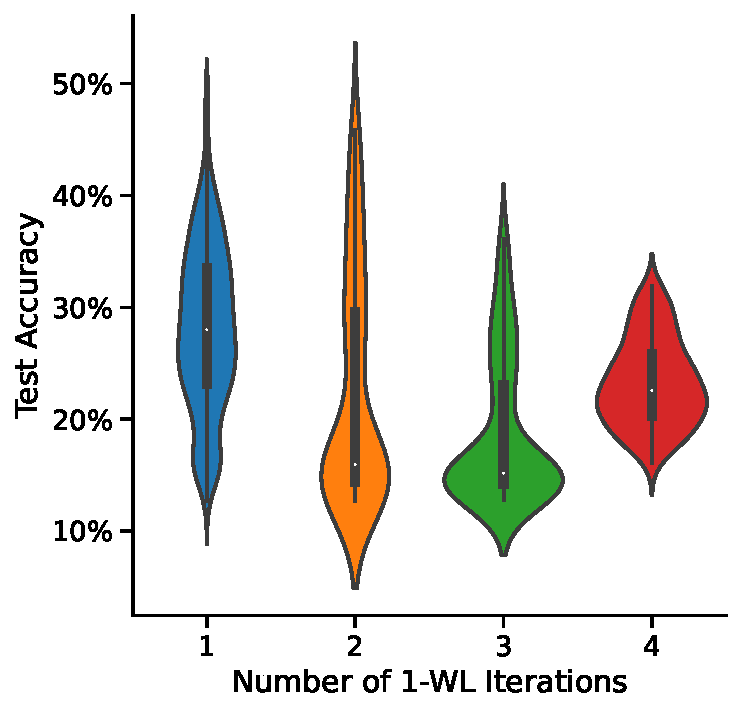
\includegraphics[width=\textwidth]{Figures/k_wl_violin_ENZYMES.pdf}
        \caption{\scriptsize\textsc{Enzymes}}
	\end{subfigure}
	\hfill
	\begin{subfigure}[b]{0.19\textwidth}
		\centering
		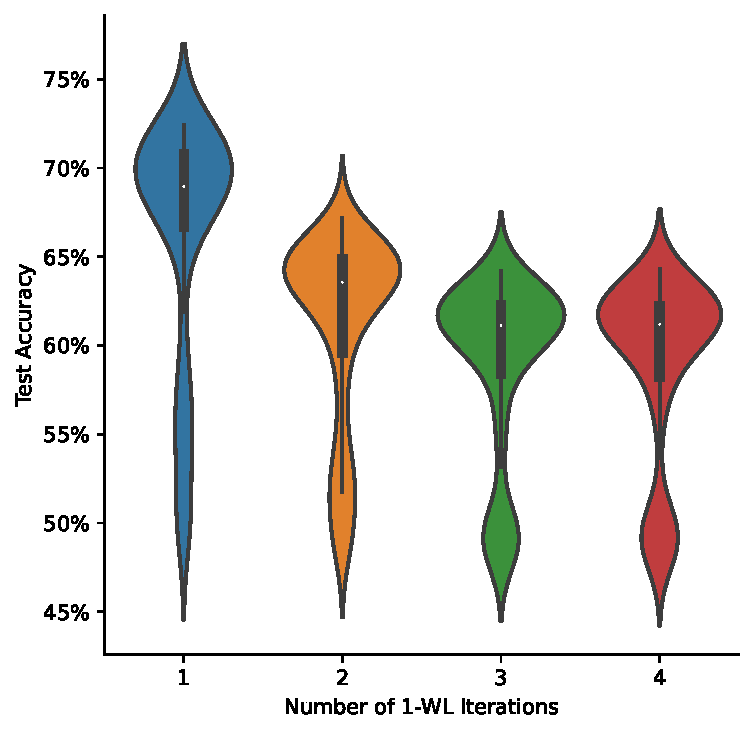
\includegraphics[width=\textwidth]{Figures/k_wl_violin_IMDB-BINARY.pdf}
        \caption{\scriptsize\textsc{Imdb-Binary}}
	\end{subfigure}
	\hfill
	\begin{subfigure}[b]{0.19\textwidth}
		\centering
		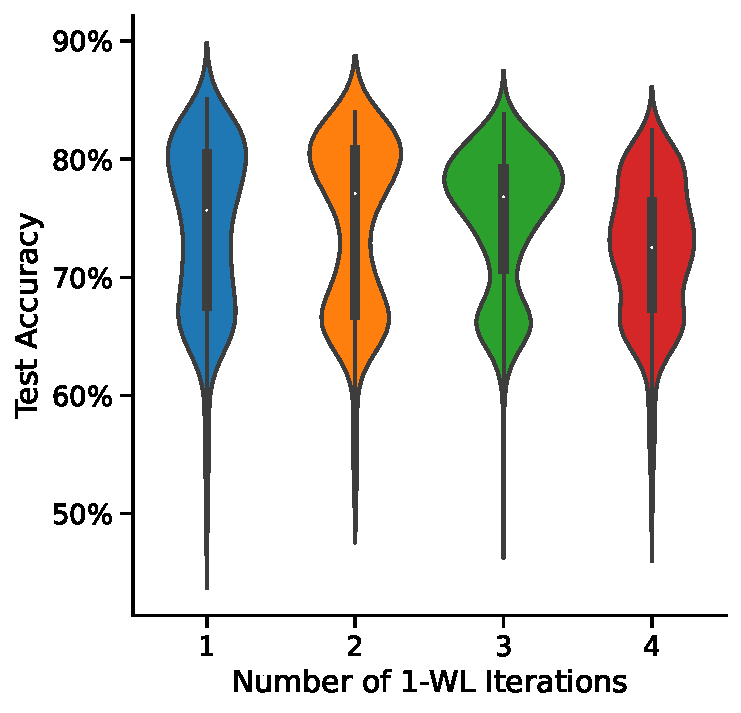
\includegraphics[width=\textwidth]{Figures/k_wl_violin_MUTAG.pdf}
        \caption{\scriptsize\textsc{Mutag}}
	\end{subfigure}
	\hfill
	\begin{subfigure}[b]{0.19\textwidth}
		\centering
		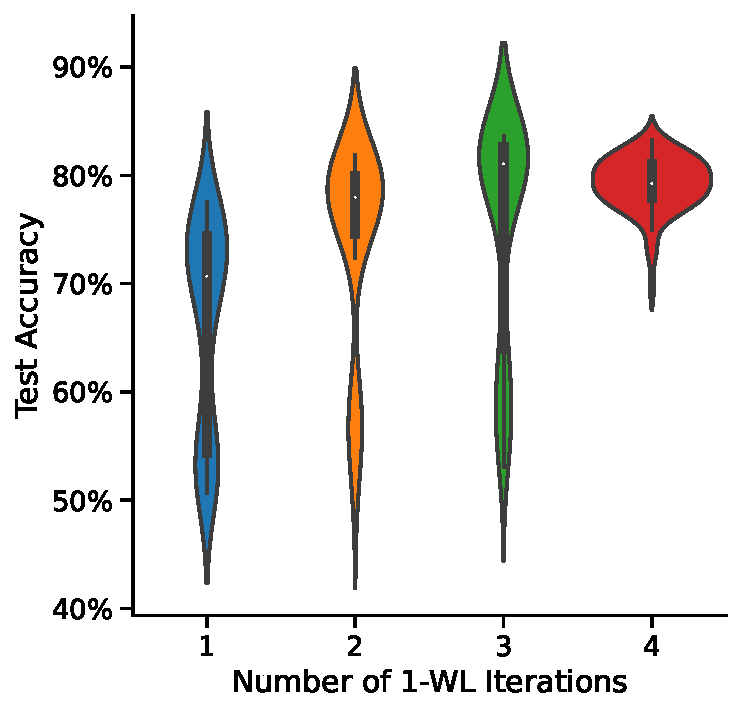
\includegraphics[width=\textwidth]{Figures/k_wl_violin_NCI1.pdf}
        \caption{\scriptsize\textsc{Nci1}}
	\end{subfigure}
	\hfill
	\begin{subfigure}[b]{0.19\textwidth}
		\centering
		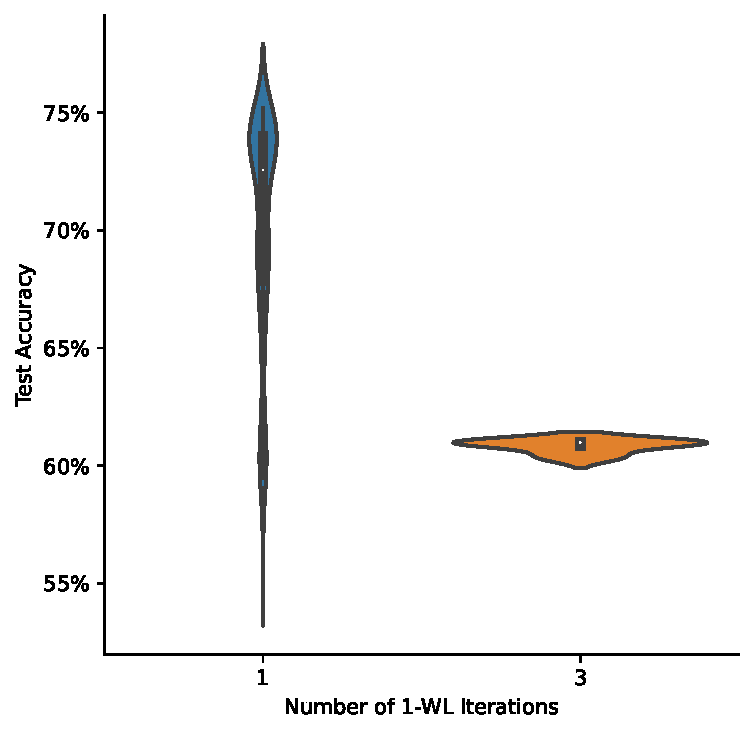
\includegraphics[width=\textwidth]{Figures/k_wl_violin_PROTEINS.pdf}
        \caption{\scriptsize\textsc{Proteins}}
	\end{subfigure}
	\par\bigskip
	\begin{subfigure}[b]{0.19\textwidth}
		\centering
		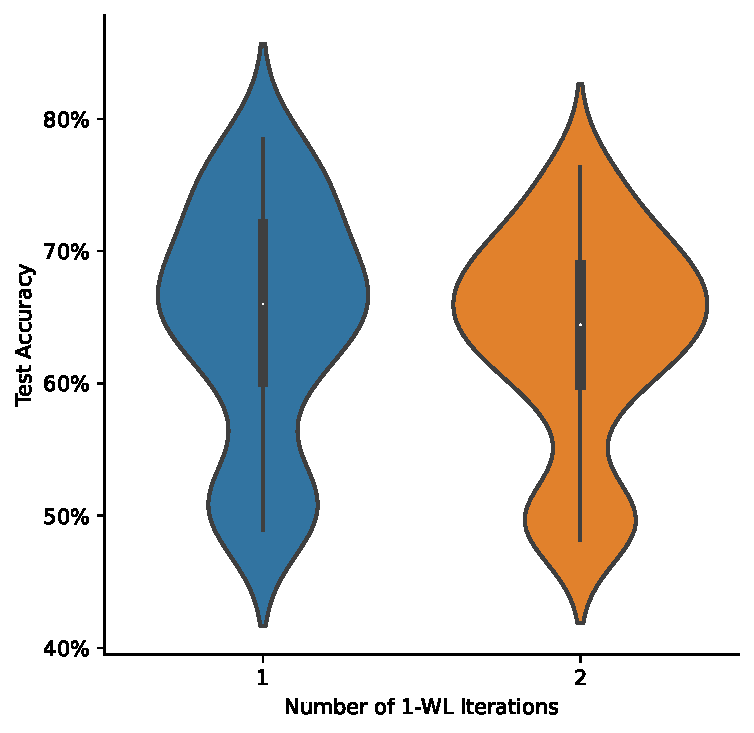
\includegraphics[width=\textwidth]{Figures/k_wl_violin_REDDIT-BINARY.pdf}
        \caption{\scriptsize \textsc{Reddit-Binary}}
	\end{subfigure}
	\hfill
	\begin{subfigure}[b]{0.19\textwidth}
		\centering
		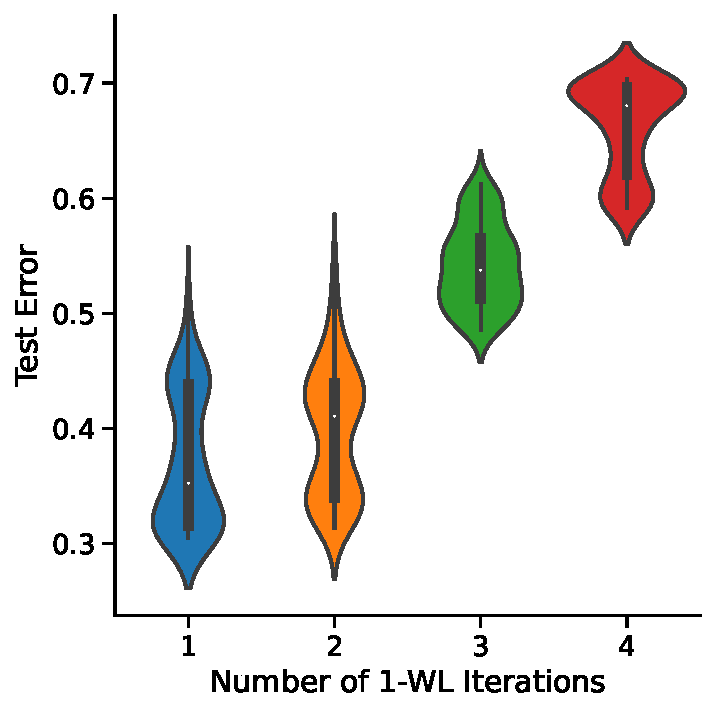
\includegraphics[width=\textwidth]{Figures/k_wl_violin_Alchemy10K.pdf}
        \caption{\scriptsize\textsc{Alchemy (10k)}}
	\end{subfigure}
	\hfill
	\begin{subfigure}[b]{0.19\textwidth}
		\centering
		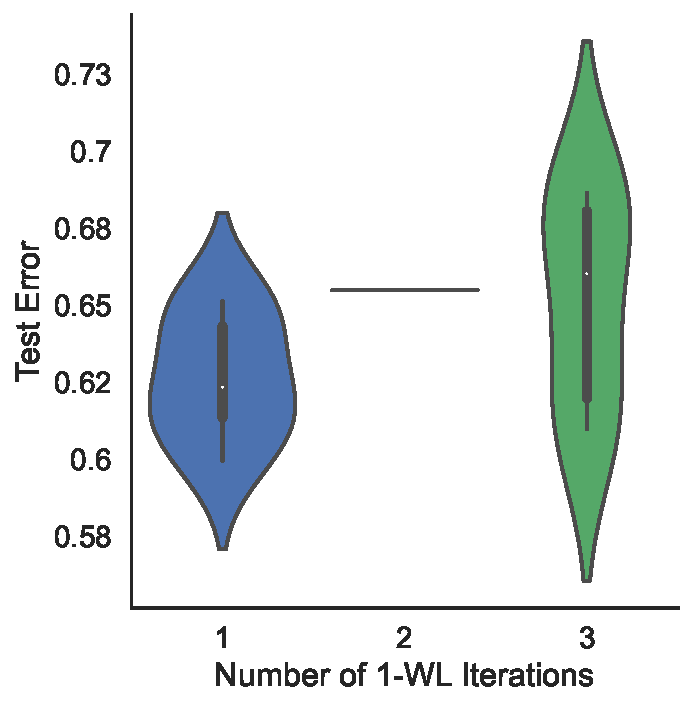
\includegraphics[width=\textwidth]{Figures/k_wl_violin_Alchemy.pdf}
        \caption{\scriptsize\textsc{Alchemy}}
	\end{subfigure}
	\hfill
	\begin{subfigure}[b]{0.19\textwidth}
		\centering
		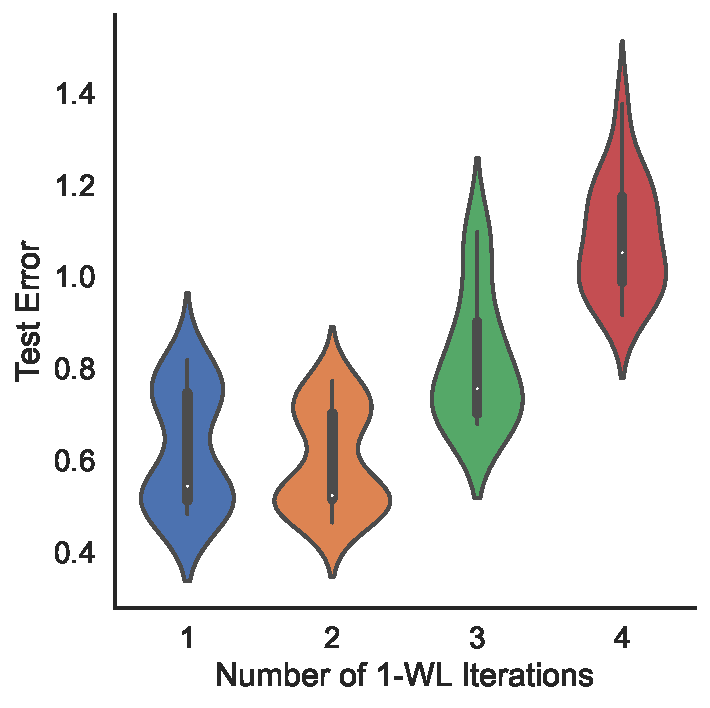
\includegraphics[width=\textwidth]{Figures/k_wl_violin_Zinc 10k.pdf}
        \caption{\scriptsize\textsc{Zinc (10k)}}
	\end{subfigure}
	\hfill
	\begin{subfigure}[b]{0.19\textwidth}
		\centering
		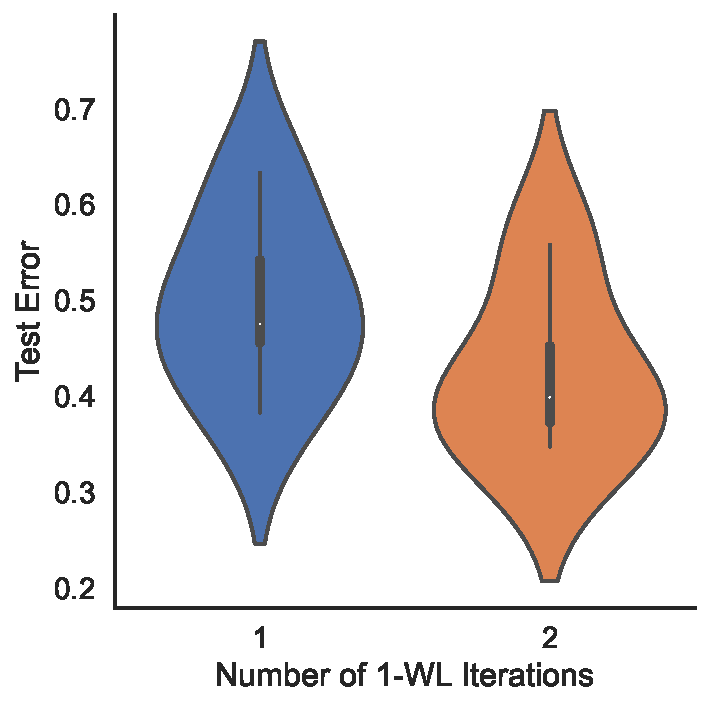
\includegraphics[width=\textwidth]{Figures/k_wl_violin_Zinc.pdf}
        \caption{\scriptsize\textsc{Zinc}}
	\end{subfigure}
	\caption{Impact on performance by the number of itertations of the \wl alogirhtm.}
	\label{fig:k_wl_dependence}
\end{figure}


\subsection{Explain how results look like}

\section{Discusssion}
\subsection{Learned Lessons}
\subsection{Future Work}

\section{Conclusion}

\newpage


\begin{table}[H]
    \resizebox{.975\textwidth}{!}{ 	\renewcommand{\arraystretch}{1.05}
		\begin{tabular}{@{}c <{\enspace}@{}lcccccc@{}}	\toprule
			& \multirow{3}{*}{\vspace*{4pt}\textbf{Method}}&\multicolumn{6}{c}{\textbf{Dataset}}\\\cmidrule{3-8}
			& & {\textsc{Enzymes}}         &  {\textsc{Imdb-Binary}}      & {\textsc{Mutag}}           & {\textsc{NCI1}}       & {\textsc{Proteins}}           & 
			{\textsc{Reddit-Binary}}
			\\
			\toprule
			\multirow{4}{*}{\rotatebox{90}{$\wlnn$}}
			& \textsf{MLP} & 48.3 \scriptsize	$\pm 8.1$ & \textbf{72.4} \scriptsize	$\pm 4.1$ & 85.1 \scriptsize $\pm 8.6$ & 83.6 \scriptsize	$\pm 4.1$ & \textbf{75.2} \scriptsize $\pm 3.9$
			\\
			& \textsf{SVM Linear} & 34.4 \scriptsize	$\pm 5.5$ & 71.2 \scriptsize	$\pm 3.9$ & 86.4 \scriptsize $\pm 8.9$	 & 83.4 \scriptsize	$\pm 2.1$ & 73.9 \scriptsize $\pm 4.1$
			\\
			& \textsf{SVM RBF} & 45.0 \scriptsize	$\pm 7.0$ & 72.8 \scriptsize	$\pm 4.3$ & 83.2 \scriptsize $\pm 7.5$ & 83.6 \scriptsize	$\pm 1.9$ & 75.2 \scriptsize $\pm 4.0$
			\\
			& \textsf{k-NN} &  \textbf{56.3} \scriptsize $\pm 5.8$ (k=1) & 72.3 \scriptsize $\pm 4.1$ (k=11)& \textbf{86.7} \scriptsize $\pm 7.7$ (k=10) & \textbf{83.9} \scriptsize $\pm 1.8$ (k=5)& 73.9 \scriptsize $\pm 4.1$ (k=19) &
			\\
			\cmidrule{2-8}
			\multirow{4}{*}{\rotatebox{90}{\gnn}}
			& \textsf{MLP} & 34.4 \scriptsize $\pm 7.0$ &  \textbf{74.7} \scriptsize $\pm 3.8$ & 84.6 \scriptsize $\pm 8.7$	 & \textbf{79.9} \scriptsize $\pm 2.2$ & 74.3 \scriptsize $\pm 5.1$
			\\
			& \textsf{SVM Linear} & 33.2 \scriptsize $\pm 5.9$ & 73.9 \scriptsize $\pm 4.2$ & 51.9 \scriptsize $\pm 34.1$ & 67.4 \scriptsize $\pm 2.2$ & 74.7 \scriptsize $\pm 4.2$
			\\
			& \textsf{SVM RBF} & 35.9 \scriptsize $\pm 6.0$ & 74.1 \scriptsize $\pm 3.9$ & \textbf{86.0} \scriptsize $\pm 7.4$ & 73.0 \scriptsize $\pm 1.9$ & 74.6 \scriptsize $\pm 4.6$
			\\ 
			& \textsf{k-NN} & \textbf{51.6} \scriptsize $\pm 7.0$ (k=1)	& 74.3 \scriptsize $\pm 4.0$ (k=132) & 88.3 \scriptsize $\pm 6.5$ (k=38) & 77.5 \scriptsize $\pm 1.7$	(k=2)& \textbf{74.9} \scriptsize $\pm 4.3$ (k=27)&
			\\
			\bottomrule
		\end{tabular}}
		\caption{Overview of the classification accuracies achieved by the best model for each dataset in percent and standard deviation. Additionally, the performance of each model was evaluated under alternative configurations, namely the substitution of the Multilayer Perceptron (MLP) with a Support Vector Machine employing either a linear kernel (SVM Linear) or the Radial Basis Function (SVM RBF), as well as the k-nearest neighbors algorithm (k-NN) with different values for $k$.}
        \label{tab:my_label3}                  
\end{table}

\begin{figure}[H]
	\begin{subfigure}[b]{0.3\textwidth}
		\centering
		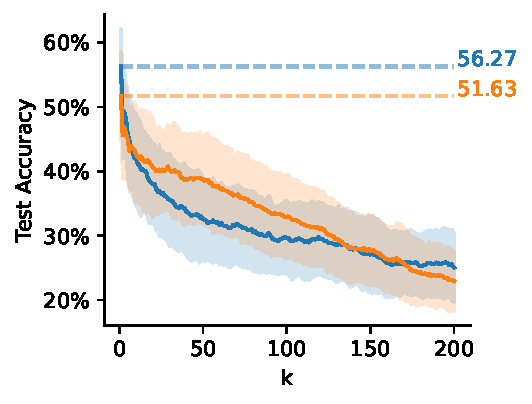
\includegraphics[width=\textwidth]{Figures/knn_ENZYMES.pdf}
		\vspace*{-4ex} 
		\caption{\textsc{Enzymes}}
	\end{subfigure}
	\hfill
	\begin{subfigure}[b]{0.3\textwidth}
		\centering
		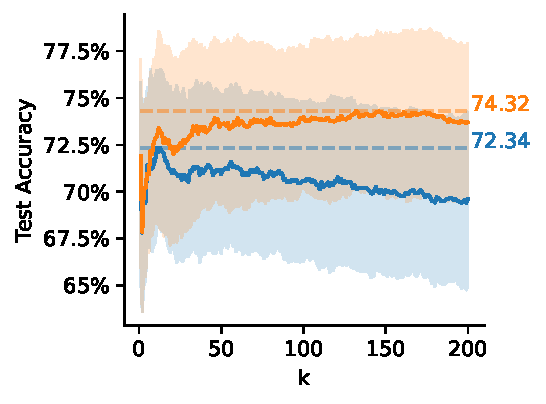
\includegraphics[width=\textwidth]{Figures/knn_IMDB-BINARY.pdf}
		\vspace*{-4ex} 
		\caption{\textsc{Imdb-Binary}}
	\end{subfigure}
	\hfill
	\begin{subfigure}[b]{0.3\textwidth}
		\centering
		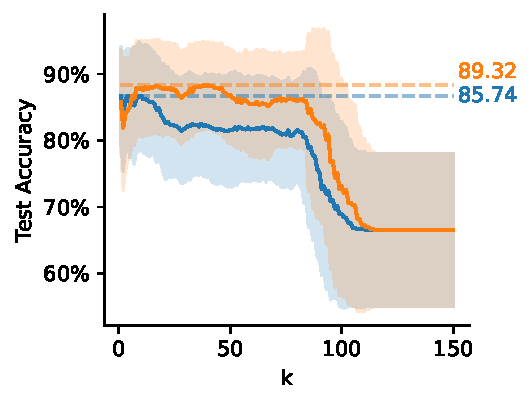
\includegraphics[width=\textwidth]{Figures/knn_MUTAG.pdf}
		\vspace*{-4ex} 
		\caption{\textsc{Mutag}}
	\end{subfigure}
	\par\bigskip
	\begin{subfigure}[b]{0.3\textwidth}
		\centering
		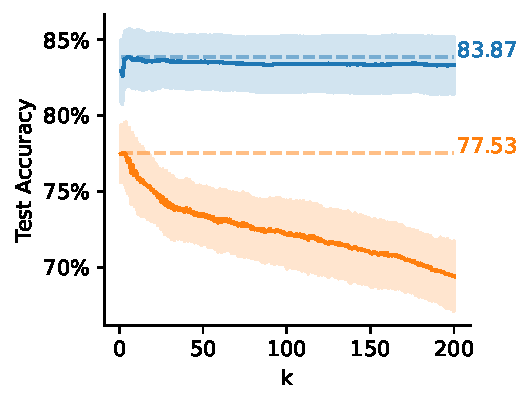
\includegraphics[width=\textwidth]{Figures/knn_NCI1.pdf}
		\vspace*{-4ex} 
		\caption{\textsc{Nci1}}
	\end{subfigure}
	\hfill
	\begin{subfigure}[b]{0.3\textwidth}
		\centering
		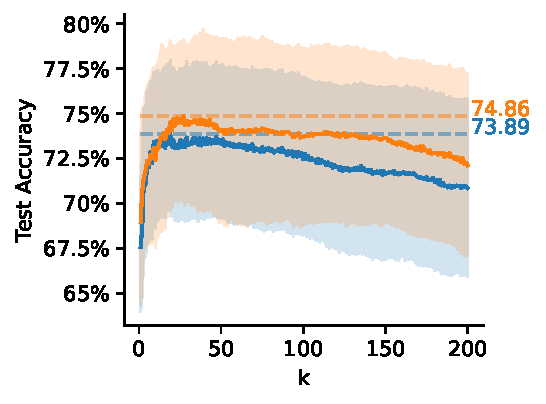
\includegraphics[width=\textwidth]{Figures/knn_PROTEINS.pdf}
		\vspace*{-4ex} 
		\caption{\textsc{Proteins}}
	\end{subfigure}
	\hfill
	\begin{subfigure}[b]{0.3\textwidth}
		\centering
		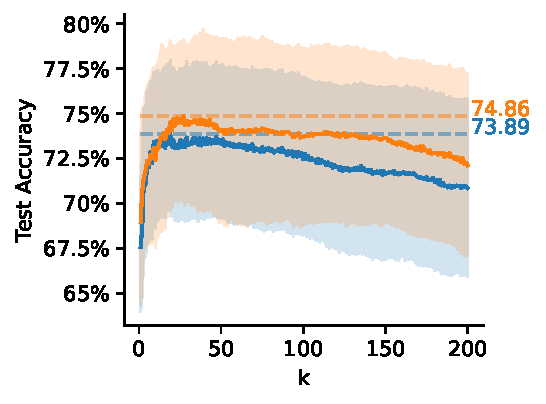
\includegraphics[width=\textwidth]{Figures/knn_PROTEINS}
		\vspace*{-4ex} 
		\caption{\textsc{Reddit-Binary}- MISSING}
	\end{subfigure}
	\centering
	\begin{subfigure}[b]{0.3\textwidth}
		\centering
		
\includegraphics[width=\textwidth]{Figures/train_test_diff_legend.pdf}
		\vspace*{-4ex} 
	\end{subfigure}
	\caption{Average classification accuracy achieved on each dataset by replacing the multilayer perceptron of the best-performing \wlnn and \gnn model with a classifier based on the $k$-nearest neighbors algorithm. We tested for different values of $k$.}
\end{figure}

\begin{figure}[H]
	\begin{subfigure}[b]{0.49\textwidth}
		\centering
		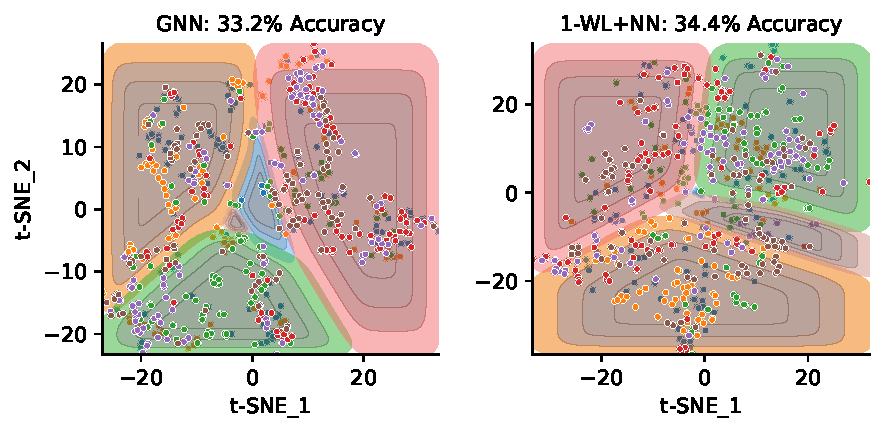
\includegraphics[width=\textwidth]{Figures/tsne_svm_lin_ENZYMES.pdf}
		\vspace*{-4ex} 
		\caption{\textsc{Enzymes}}
	\end{subfigure}
	\hfill
	\begin{subfigure}[b]{0.49\textwidth}
		\centering
		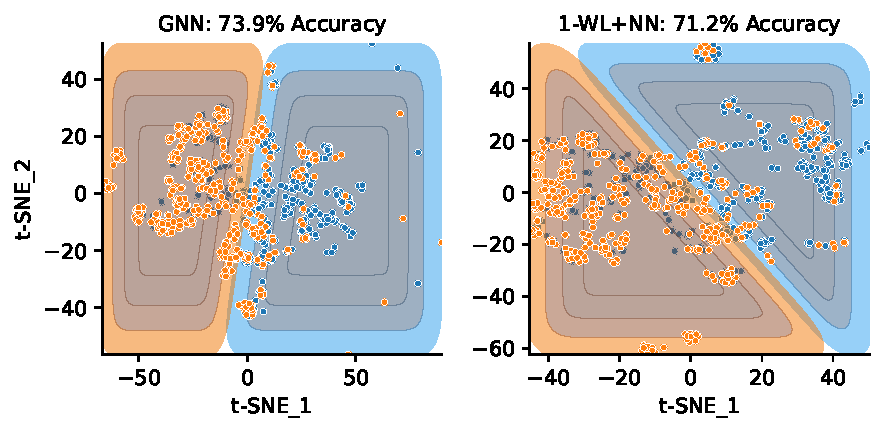
\includegraphics[width=\textwidth]{Figures/tsne_svm_lin_IMDB.pdf}
		\vspace*{-4ex} 
		\caption{\textsc{Imdb-Binary}}
	\end{subfigure}
	\par\bigskip
	\begin{subfigure}[b]{0.49\textwidth}
		\centering
		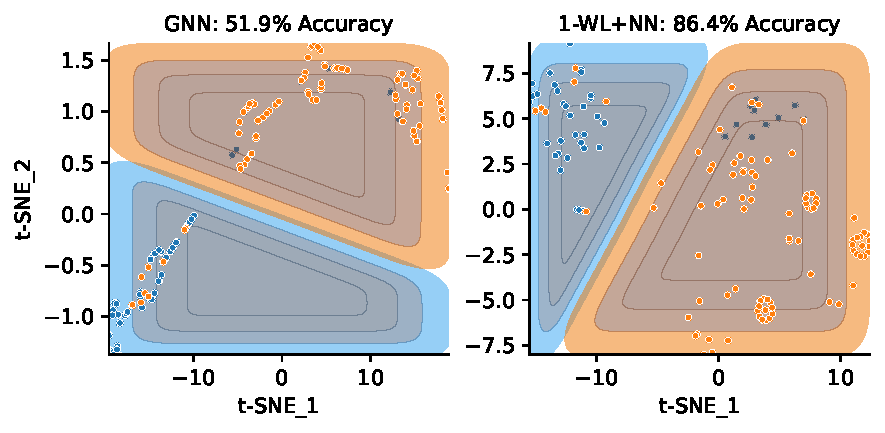
\includegraphics[width=\textwidth]{Figures/tsne_svm_lin_MUTAG.pdf}
		\vspace*{-4ex} 
		\caption{\textsc{Mutag}}
	\end{subfigure}
	\hfill
	\begin{subfigure}[b]{0.49\textwidth}
		\centering
		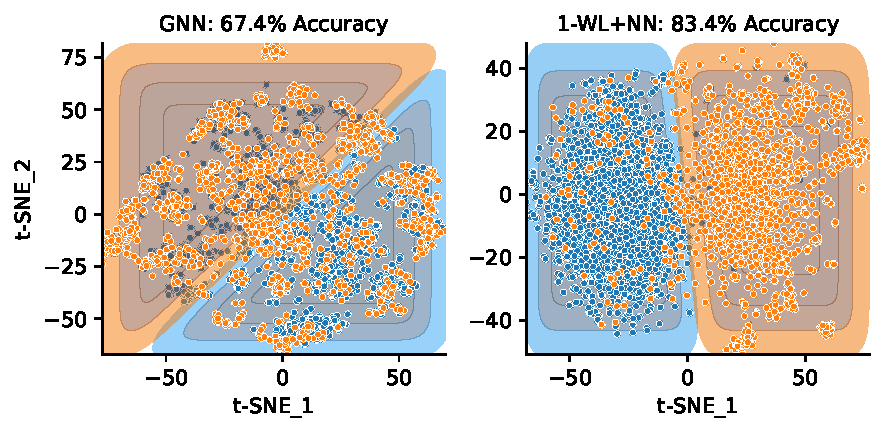
\includegraphics[width=\textwidth]{Figures/tsne_svm_lin_NCI1.pdf}
		\vspace*{-4ex} 
		\caption{\textsc{Nci1}}
	\end{subfigure}
	\par\bigskip
	\begin{subfigure}[b]{0.49\textwidth}
		\centering
		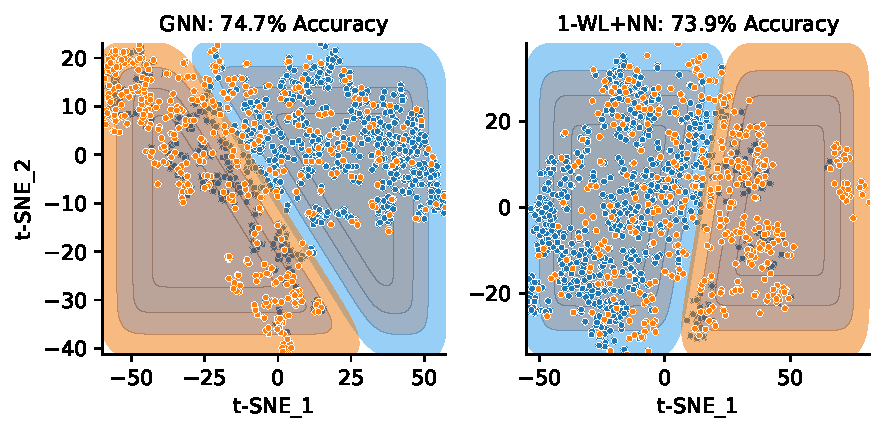
\includegraphics[width=\textwidth]{Figures/tsne_svm_lin_PROTEINS.pdf}
		\vspace*{-4ex} 
		\caption{\textsc{Proteins}}
	\end{subfigure}
	\hfill
	\begin{subfigure}[b]{0.49\textwidth}
		\centering
		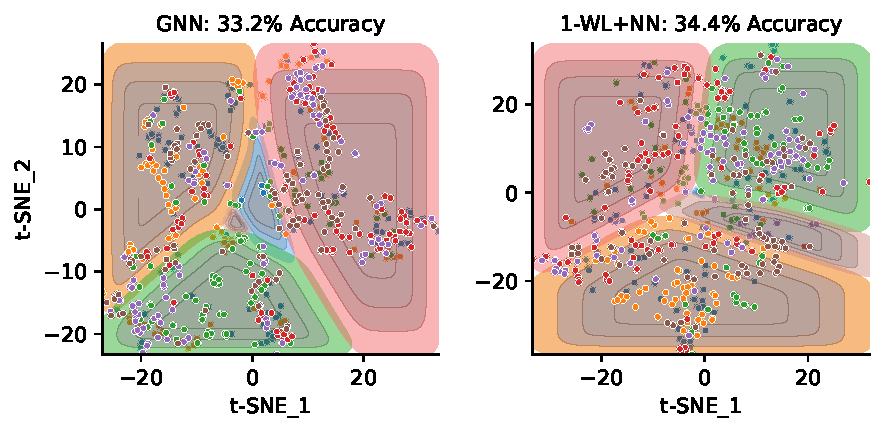
\includegraphics[width=\textwidth]{Figures/tsne_svm_lin_ENZYMES.pdf}
		\vspace*{-4ex} 
		\caption{\textsc{Reddit-Binary}- MISSING!}
	\end{subfigure}
	\caption{Visualization of the decision boundary of each Support Vector Machine with a linear kernel using t-SNE.}
\end{figure}

\begin{figure}[H]
	\centering
	\begin{subfigure}[b]{0.49\textwidth}
		\centering
		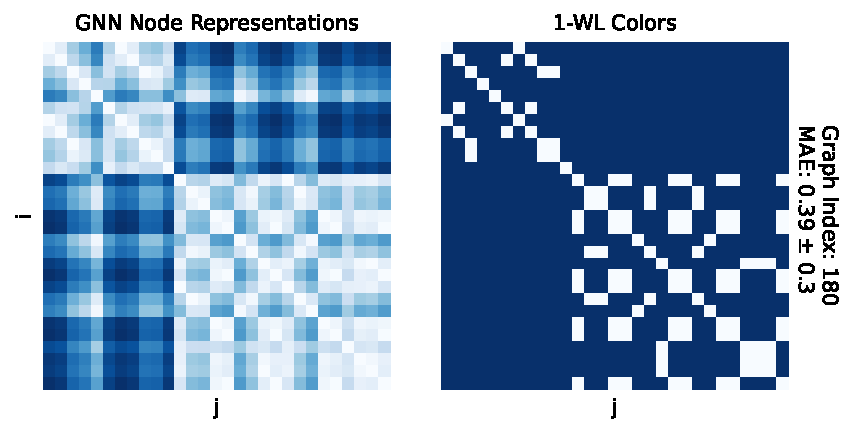
\includegraphics[width=\textwidth]{Figures/heatmaps_ENZYMES_single.pdf}
		\vspace*{-5ex} 
        \caption{\textsc{Enzymes}}
	\end{subfigure}
	\hfill
	\begin{subfigure}[b]{0.49\textwidth}
		\centering
		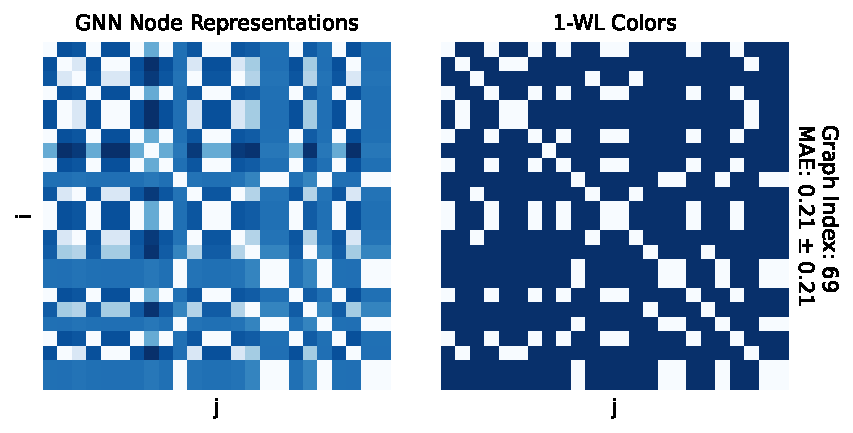
\includegraphics[width=\textwidth]{Figures/heatmaps_IMDB-BINARY_single.pdf}
		\vspace*{-5ex} 
        \caption{\textsc{Imdb-Binary}}
	\end{subfigure}
	\par\bigskip
	\begin{subfigure}[b]{0.49\textwidth}
		\centering
		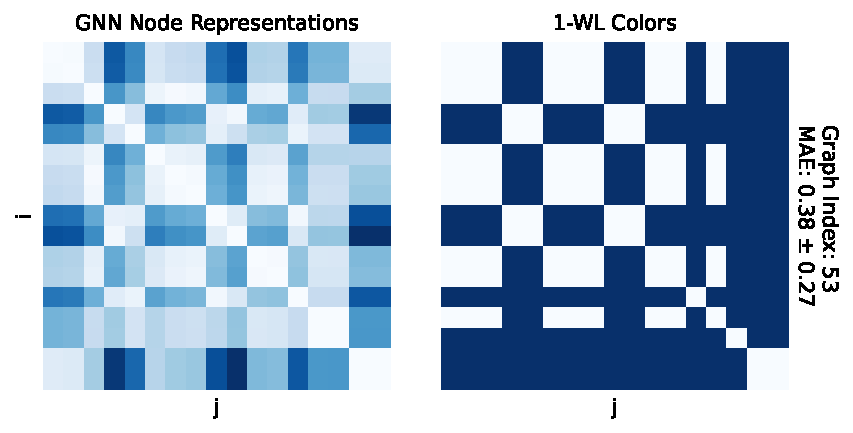
\includegraphics[width=\textwidth]{Figures/heatmaps_MUTAG_single.pdf}
		\vspace*{-5ex} 
        \caption{\textsc{Mutag}}
	\end{subfigure}
	\hfill
	\begin{subfigure}[b]{0.49\textwidth}
		\centering
		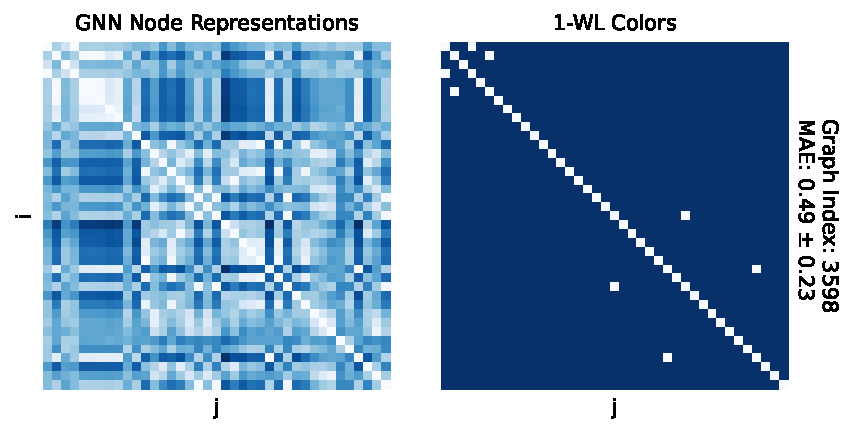
\includegraphics[width=\textwidth]{Figures/heatmaps_NCI1_single.pdf}
		\vspace*{-5ex} 
        \caption{\textsc{Nci1}}
	\end{subfigure}
	\par\bigskip
	\begin{subfigure}[b]{0.49\textwidth}
		\centering
		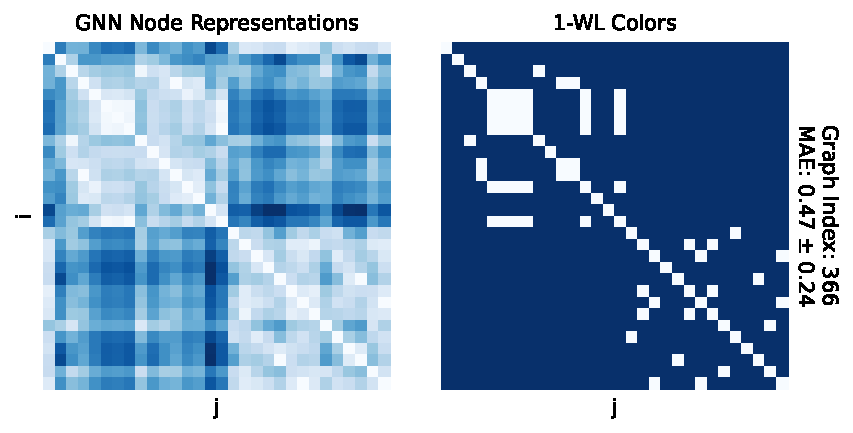
\includegraphics[width=\textwidth]{Figures/heatmaps_PROTEINS_single.pdf}
		\vspace*{-5ex} 
        \caption{\textsc{Proteins}}
	\end{subfigure}
	\hfill
	\begin{subfigure}[b]{0.49\textwidth}
		\centering
		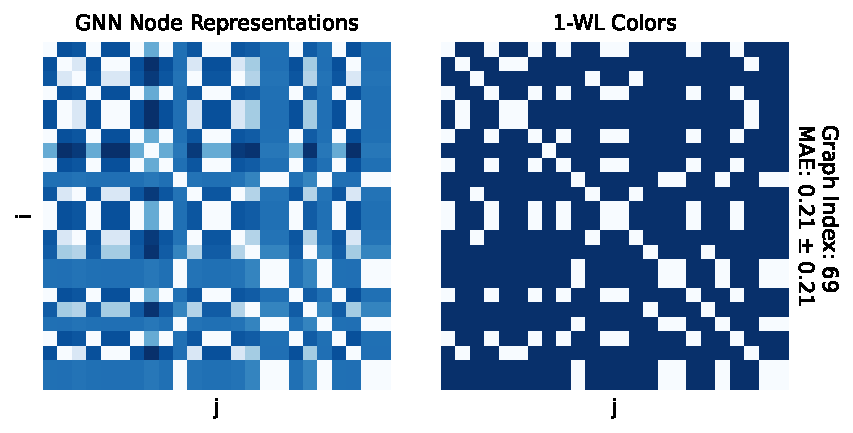
\includegraphics[width=\textwidth]{Figures/heatmaps_IMDB-BINARY_single.pdf}
		\vspace*{-5ex}
        \caption{\textsc{Reddit-Binary}-MISSING}
	\end{subfigure}
	\par\bigskip
	\begin{subfigure}[b]{0.6\textwidth}
		\centering
		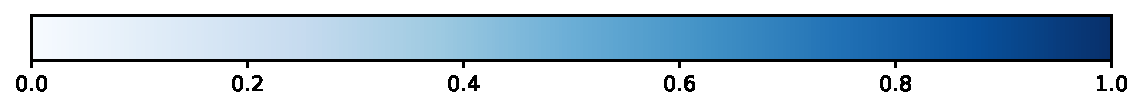
\includegraphics[width=\textwidth]{Figures/colorbar.pdf}
	\end{subfigure}
	\caption{Visualizing the performance of the best-performing \gnn models of each dataset in approximating node colors computed by the \wl algorithm. Here we randomly sampled a single graph for each dataset and visualized the approximation performance. For each calculation of the \wl colors, we utilized the number of iterations of the \wl algorithm to be the same as the best-performing \wlnn model of each dataset. Specifically, this was 1 for all datasets except for \textsc{Nci1}, where it was 3.}
\end{figure}

\begin{table}[H]
    \resizebox{.975\textwidth}{!}{ 	\renewcommand{\arraystretch}{1.05}
		\begin{tabular}{@{}c <{\enspace}@{}lcccccc@{}}	\toprule
			& \multirow{2}{*}{\vspace*{4pt}\textbf{Property}}&\multicolumn{6}{c}{\textbf{Dataset}}\\\cmidrule{3-8}
			& & {\textsc{Enzymes}}         &  {\textsc{Imdb-Binary}}      & {\textsc{Mutag}}           & {\textsc{NCI1}}       & {\textsc{Proteins}}           & 
			{\textsc{Reddit-Binary}}
			\\
			\toprule
			\multirow{1}{*}{}
			& MAE & 0.49 \scriptsize $\pm 0.3$ & 0.14 \scriptsize $\pm 0.15$ & 0.42 \scriptsize $\pm 0.29$
			& 0.42 \scriptsize $\pm 0.22$ & 0.49 \scriptsize $\pm 0.26$
			\\
			& Number of \wl colors & 230 & 64 & 32 & 27252 & 296 &
			\\
			\bottomrule
		\end{tabular}}
		\caption{MAE of the approximation performance of the best-perfoming \gnn in relation to the number of unique \wl colors for each dataset. In particular, in comparison to the colors computed by the \wl alogrithm with a single iteration.}
        \label{tab:my_label4}     
\end{table}

\begin{table}[H]
    \resizebox{.975\textwidth}{!}{ 	\renewcommand{\arraystretch}{1.05}
		\begin{tabular}{@{}c <{\enspace}@{}lcccccc@{}}	\toprule
			& \multirow{2}{*}{\vspace*{4pt}\textbf{Epsilon}}&\multicolumn{6}{c}{\textbf{Dataset}}\\\cmidrule{3-8}
			& & {\textsc{Enzymes}}         &  {\textsc{Imdb-Binary}}      & {\textsc{Mutag}}           & {\textsc{NCI1}}       & {\textsc{Proteins}}           & 
			{\textsc{Reddit-Binary}}
			\\
			\toprule
			\multirow{4}{*}{\rotatebox{90}{F1-Score}}
			& $\epsilon = 0.001$ & 52.55 & 60.97 & 62.01 &
			\\
			& $\epsilon = 0.01$ & 54.63 & 60.97 & 62.01 &
			\\
			& $\epsilon = 0.05$ & 62.33 & 71.68 & 62.01 & 
			\\
			& $\epsilon = 0.1$ & 70.45 & 78.66 & 62.01 &
			\\
			\cmidrule{2-8}
			& Number of \wl colors & 230 & 64 & 32 & 27252 & 296 &
			\\
			\bottomrule
		\end{tabular}}
		\caption{MAE of the approximation performance of the best-perfoming \gnn in relation to the number of unique \wl colors for each dataset. In particular, in comparison to the colors computed by the \wl alogrithm with a single iteration.}
        \label{tab:my_label4}     
\end{table}

\begin{figure}[H]
	\begin{subfigure}[b]{0.3\textwidth}
		\centering
		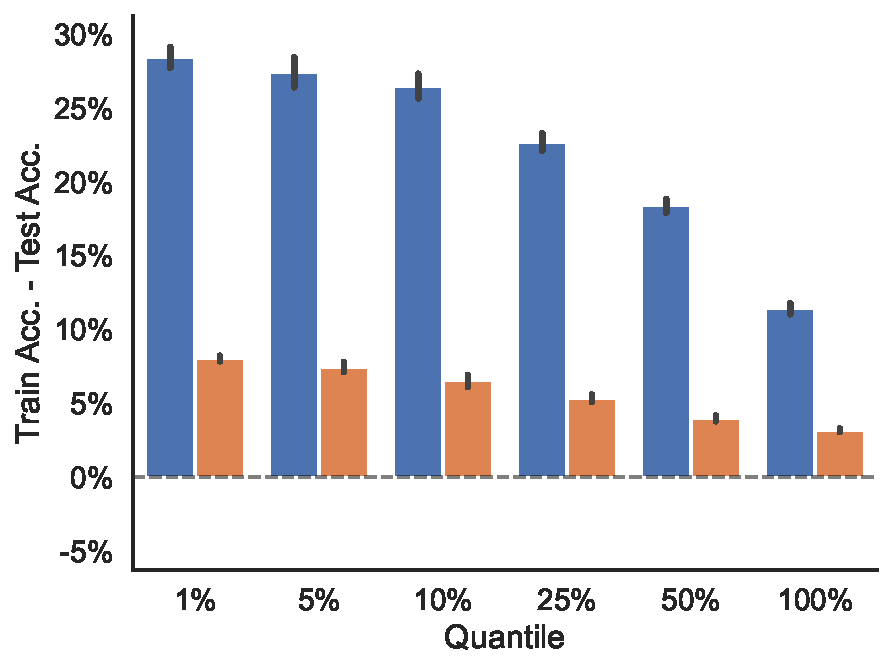
\includegraphics[width=\textwidth]{Figures/train_test_diff_ENZYMES.pdf}
		\vspace*{-4ex} 
		\caption{\textsc{Enzymes}}
	\end{subfigure}
	\hfill
	\begin{subfigure}[b]{0.3\textwidth}
		\centering
		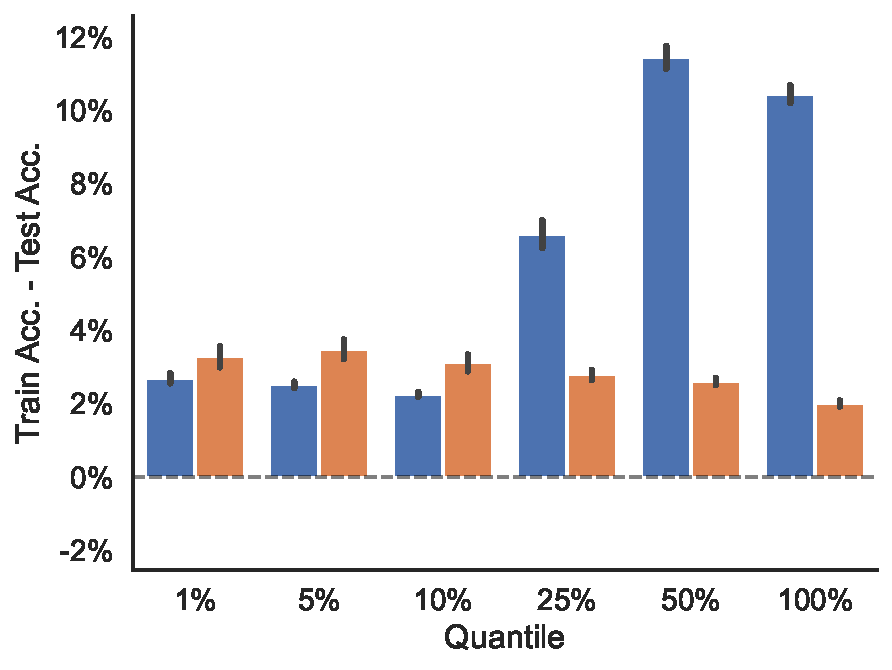
\includegraphics[width=\textwidth]{Figures/train_test_diff_IMDB-BINARY.pdf}
		\vspace*{-4ex} 
		\caption{\textsc{Imdb-Binary}}
	\end{subfigure}
	\hfill
	\begin{subfigure}[b]{0.3\textwidth}
		\centering
		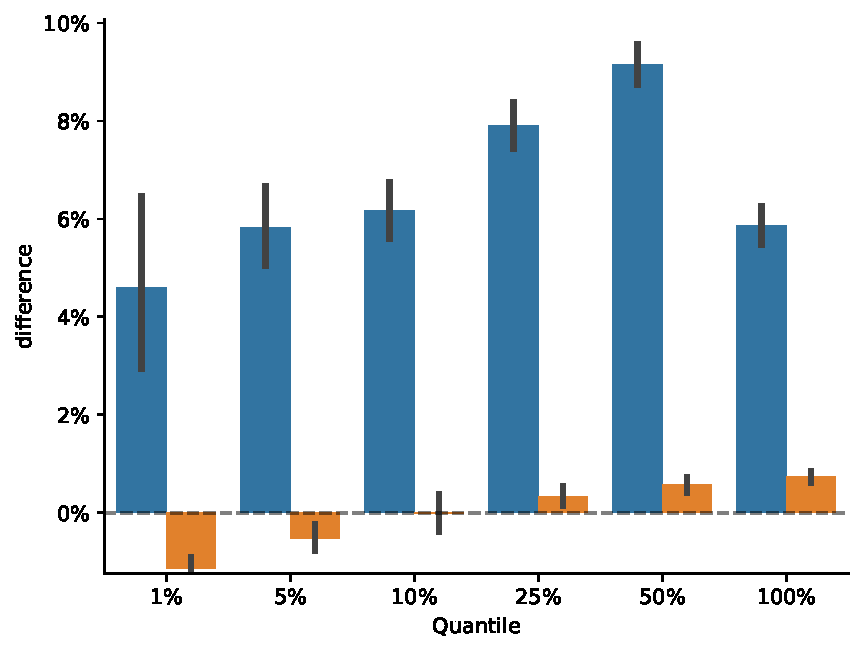
\includegraphics[width=\textwidth]{Figures/train_test_diff_MUTAG.pdf}
		\vspace*{-4ex} 
		\caption{\textsc{Mutag}}
	\end{subfigure}
	\par\bigskip
	\begin{subfigure}[b]{0.3\textwidth}
		\centering
		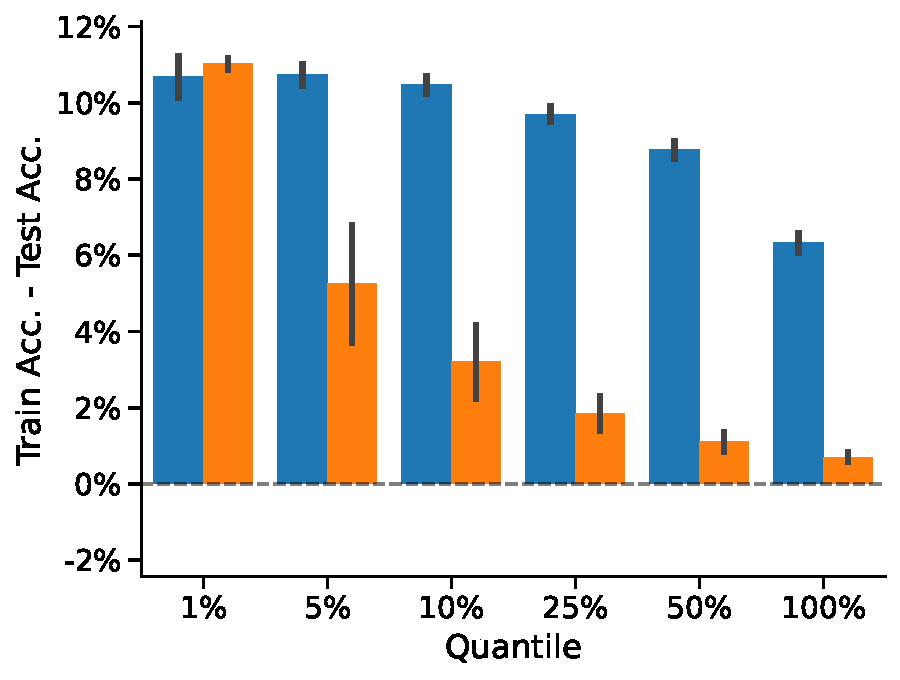
\includegraphics[width=\textwidth]{Figures/train_test_diff_NCI1.pdf}
		\vspace*{-4ex} 
		\caption{\textsc{Nci1}}
	\end{subfigure}
	\hfill
	\begin{subfigure}[b]{0.3\textwidth}
		\centering
		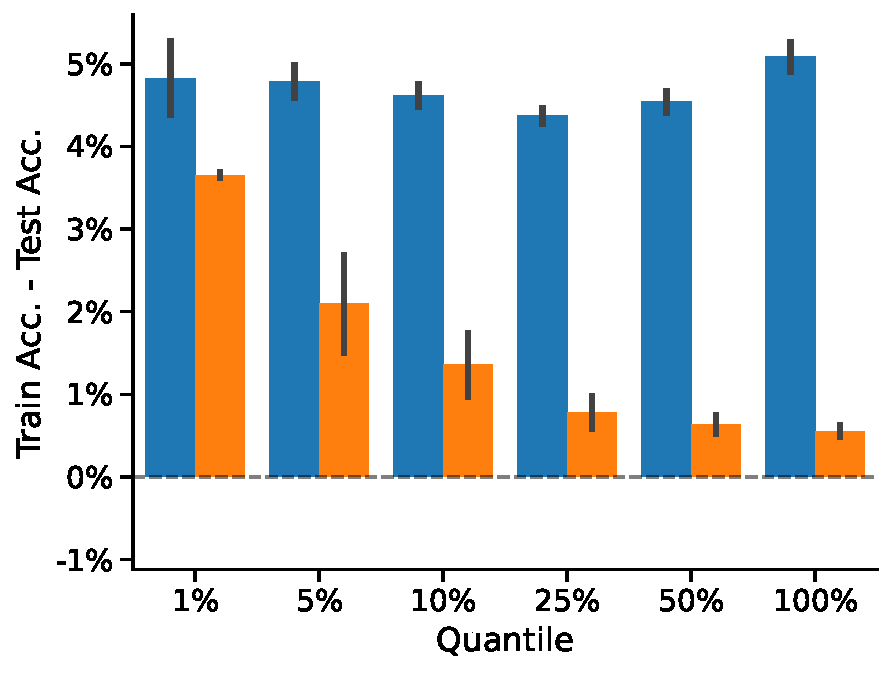
\includegraphics[width=\textwidth]{Figures/train_test_diff_PROTEINS.pdf}
		\vspace*{-4ex} 
		\caption{\textsc{Proteins}}
	\end{subfigure}
	\hfill
	\begin{subfigure}[b]{0.3\textwidth}
		\centering
		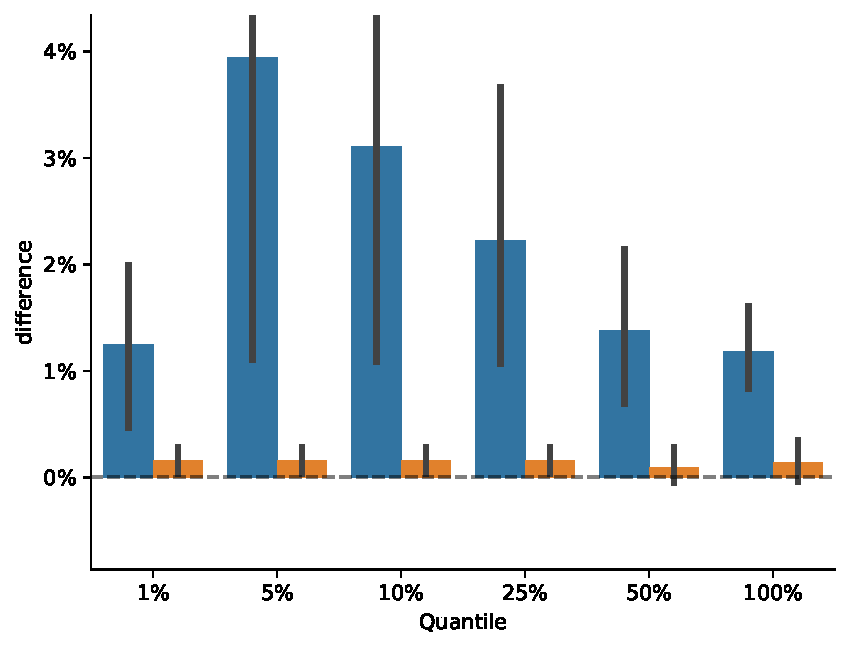
\includegraphics[width=\textwidth]{Figures/train_test_diff_REDDIT-BINARY.pdf}
		\vspace*{-4ex} 
		\caption{\textsc{Reddit-Binary}}
	\end{subfigure}
	\centering
	\begin{subfigure}[b]{0.3\textwidth}
		\centering
		
\includegraphics[width=\textwidth]{Figures/train_test_diff_legend.pdf}
		\vspace*{-4ex} 
	\end{subfigure}
	\caption{Mean absolute difference of the classification accuracies of the training and testing set of each dataset. In detail, we compared the different quantiles of each performance.}
\end{figure}

\chapter{These / Narrativ}
\begin{enumerate}
	\item \wlnn funktioniert nur sehr gut auf kleinen datasets:
	\begin{itemize}
		\item  Je größer das Dataset desto größer wird die 1-WL-Color ``Vielfalt'', schwierig für das MLP des \wlnn noch die richtigen Information rauszuziehen. -> These würde ich gerne noch überprüfen: Gibt es ein Classification Dataset das groß und gut ist? OGBG-Molhiv? MalNet Tiny?
		\item Dagegenspricht aber das die performance von NCI1 deutlich besser ist von \wlnn.
		\item Theorie warum \wlnn aktuell fast immer besser war, ist dass \wlnn viel weniger Parameter optimieren muss bei gleicher im Vergleich zu GNNs -> Optimum ist schneller gefunden!
		\item \gnn generalisieren besser im Sinne, dass sie unabhängig von der größe des Datasets sind. Alchemy zeigt das ganz gut!
		\item Difference in Training and Test Accuracy zeigt auch das die \wlnn Modelle stark overfitten -> Tendenz dazu dass mit größeren Datasets, generalisieren schwieriger wird.
		\item Performance von den \wlnn Modellen ohne Embedding (Look-Up-Table) ist auch nur auf kleinen Datasets gut. Je größer das Dataset desto größer ist die Differenz zwischen beiden Modell Konfigurationen.
	\end{itemize}
	\item GNNs approximiert \wl Farben:
	\begin{itemize}
		\item Aprroximation ist vorhanden und ist nicht so schlecht: Error ist zwar so circa bei 50\% dafür ist die std aber auch sehr hoch (circa 25\%).
		\item Vorallem approximierung von \wl mit nur einer Iteration (Node Degree!)
		\item Performance von den GNNs mit Node-degree initialiserung sind bis jetzt immer besser gewesen (IMDB-Binary \& Reddit-Binary)
	\end{itemize}
	\item GNNs und \wlnn erlernen graph representation die gut clustern:
	\begin{enumerate}
		\item Sehr gute lineare Separierbarkeit bei allen Datsets (Ausnahme ist Mutag wegen Bug!)
		\item k-NN clustering hoch für kleine k's bei beiden Modellen. Sehr ähnliche Accuracy Kurven!
		\item (t-SNE plots zeigen auch, dass clustering vorhanden ist.)
	\end{enumerate}
\end{enumerate}

		
F1  metric oder ROC (watch out unbalanced dataset)

-> intuition: gnn smoothen! (noise reduction)-> \gnn optimalere funktionen
Setup: de-noising notwendig, CSWM Problem konzipieren -> erst de-noising befor gute prediction


\setcitestyle{numbers}
\bibliography{references}

\newpage
\appendix
\chapter{Appendix Part I}
\section{Figures and graphs}


\section{Proofs}

\subsection{\cref{lem:composition_lemma}: Composition Lemma for $\wlnn$}\label{app:composition_proof}
Before we begin with the actual compositon proof, we give a formal defintion and notation for MLPs.

\begin{definition}[Multilayer Perceptron]\label{def:mlp}
    Multilayer perceptrons are a class of functions from $\Rb^n$ to $\Rb^m$, with $n,m \in \Nb$. In this thesis, we define a multilayer perceptron as a finite sequence, such that a multilayer perceptron $\mlp$ is defined as $\mlp \coloneqq (\mlp)_{i\in[k]}$ where $k$ is the number of layers. For every $i \in [k]$, the $i$.th layer of the $\mlp$ is the $i$.th item in the finite sequence $\mlp_i$. Further, all layers are recursively defined as: \todo{Adapt the notation for sequences $(\mlp_i)_{i \in [k]}$}
    \begin{align*}
        \mlp_{0}(v) &\coloneqq v\\
        \mlp_{i+1}(v) &\coloneqq \sigma_i(W_i \cdot \mlp_{i} (v) + b_i), \quad \forall i \in [k-1]
    \end{align*}
    where $\sigma_i$ is an element wise activation function, $W_i$ is the weight matrix and $b_i$ the bias vector of layer $i$. Note, that for each $W_i$, the succeeding $W_{i+1}$ must have the same number of columns as $W_i$ has rows, in order to be well-defined. Similarly, for every layer $i$, $W_i$ and $b_i$ have to have the same number of rows.
    Following this definition, when applying a $\mlp$ on input $v \in \Rb^n$ it is $\mlp(v) \coloneqq (\mlp)_k(v)$.
\end{definition}

\begin{proof}[Proof of \cref{lem:composition_lemma}]
    Let $\cC$ be a collection of functions computed by $\wlnn$, $h_1, \dots ,h_n \in \cC$, and $\mlp^\bullet$ a multilayer perceptron. Further, let $f_{1}, \ldots, f_{n}$ be the encoding functions, as well as $\text{MLP}_1, \ldots, \text{MLP}_n$ be the multilayer perceptrons used by $h_1, \dots h_n$ respectively. As outlined above, we will now construct $f^*$ and $\mlp^*$, such that for all graphs $G \in \cX$:
    \begin{equation*}
        \mlp^\bullet(h_1(G), \dots ,h_n(G)) = \mlp^* \circ f^* (\MSopen \wl(G)(v) \mid v \in V(G) \MSclose)
    \end{equation*}
    with which we can conclude that the composition of multiple functions computable by $\wlnn$, is in fact also $\wlnn$ computable. 

    We define the new encoding function $f^*$ to work as follows on an arbitrary input multiset $M$:
    \begin{equation*}
        f^*(M) := \textsf{concat}(
            \begin{bmatrix}
                f_1(M)\\
                \vdots\\
                f_n(M)
            \end{bmatrix}),
    \end{equation*}
    where $\textsf{conccat}$ is the concatenation function, concatenating all encoding vectors to one single vector.

   Using the decomposition introduced in \cref{def:mlp}, we can decompose each $\mlp_i$ for $i \in [n]$ at layer $j > 0$ as follows: $(\mlp_i)_{j}(v) := \sigma_{i,t}(W^{i}_{j} \cdot (\mlp_i)_{j-1}(v) + b^i_j)$. Using this notation we construct $\mlp^*$ as follows:
    \begin{align*}
        &(\mlp^*)_{0}(v) := v\\
        &(\mlp^*)_{j+1}(v) := \sigma^*_j(W^*_j \cdot (\mlp^*)_{j} (v) + \textsf{concact}(
            \begin{bmatrix}
                b^1_j\\
                \vdots\\
                b^n_j
            \end{bmatrix})) &,\forall j \in [k]\\
        &(\mlp^*)_{j+k+1}(v) := (\mlp^\bullet)_{j+1}(v) &,\forall j \in [k^\bullet - 1]
    \end{align*}
    where $k$ is the maximum number of layers of the set of $\mlp_i$'s, and $k^\bullet$ is the number of layers of the given $\mlp^\bullet$. Thereby, we define in the first equation line, that the start of the sequence is the input, with the second line, we construct the ``simultaneous'' execution of the $\mlp_i$'s, and in the last equation line, we add the layers of the given $\mlp^\bullet$ to the end. Further, we define the weight matrix $W_j^*$ as follows: 
    \begin{align*}
        W^*_j &:= \begin{bmatrix}
            W^1_j & 0 & \hdots & 0\\
            0 & W^2_j & \ddots & \vdots\\
            \vdots & \ddots & \ddots & 0\\
            0 & \hdots & 0 & W^n_j
        \end{bmatrix},
    \end{align*}
    such that we build a new matrix where each individual weight matrix is placed along the diagonal. Here we denote with ``$0$'' zero matrices with the correct dimensions, such that $W_j^*$ is well-defined. Important to note, should for an $\mlp_i$, $W^i_j$ not exist, because it has less than $j$ layers, we use for $W^i_j$ the identity matrix $I_m$ where $m$ is the dimension of the output computed by $\mlp_i$. And finally, we define the overall activation function $\sigma^*_j$ as following:
    \begin{equation*}
        \sigma^*_j(v) := \begin{bmatrix}
            \sigma_{1,j}(v[1])\\
            \vdots\\
            \sigma_{1,j}(v[d_1])\\
            \vdots\\
            \sigma_{n,j}(v[d_1 + \dots + d_{n-1} + 1])\\
            \vdots\\
            \sigma_{n,j}(v[d_1 + \dots + d_{n}])
        \end{bmatrix},
    \end{equation*}
    where $d_i$ is the dimension of the output of $\mlp_i$ at layer $j$, and for the ease of readability we denote the $i$.th component of vector $v$ here with $v[i]$. Thereby, we construct an activation function that applies each respective activation function of the $\mlp_i$'s individually to their respective computation.
\end{proof}

\chapter{Appendix Part II}
\section{Definitions}
\subsection{Definition of the normalized Shannon Index}\label{sec:definition_shannon_index}
We calculate the normalized Shannon index as follows:
\begin{equation}
	- \frac{1}{\log_2(|C|)} \cdot \nsum_{i \in C} \frac{n_i}{n} \cdot \log_2 (\frac{n_i}{n})
\end{equation}
where $n$ is the total number of samples of the dataset, $C$ is the set of all classes, and $n_i$ is the number of samples of the class $i \in C$. As an example, for the dataset \textsc{Proteins} the variables are set to be the following: $C = \{0, 1\}$ with $n_0 = 663$ and $n_1 = 450$, so that $n = 1113$, yielding a rounded value of $0.973$.

\subsection{Theoretical Maximum Accuracy Analysis}

\begin{table}[H]
	\caption{An overview of the maximum theoretical classification accuracy achievable for each dataset based on the number of 1-WL iterations in percent. A hyphen ``-'' indicates that the maximum accuracy has converged with fewer iterations, implying that further iterations do not improve the accuracy. ``\textsc{Oom}'' denotes out of memory error.}
    \centering
	\label{tab:max_accuracies_app}
		\begin{tabular}{@{}c <{\enspace}@{}lcccccc@{}}	\toprule
			& \multirow{3}{*}{\vspace*{4pt}\textbf{Datasets}}&\multicolumn{6}{c}{\textbf{Number of iterations of the \wl algorithm}}\\\cmidrule{3-8}
			& & {0}  & {1}  & {2}  & {3} & {4}  & {5}
			\\
			\toprule

			\multirow{4}{*}{\rotatebox{90}{Bioinformatics}}
            & DD &1.00 & - & - & - & - & - \\
            & ENZYMES &0.81 & 1.00 & - & - & - & - \\
            & KKI & 1.00 & - & - & - & - & - \\
            & OHSU & 1.00 & - & - & - & - & - \\
            & Peking\_1 & 1.00 & - & - & - & - & - \\
            & PROTEINS &0.92 & 1.00 & - & - & - & -\\

            % \cmidrule{2-8}
            % \multirow{1}{*}{\rotatebox{90}{C}}
            % & COIL-DEL \\

            \cmidrule{2-8}
            \multirow{9}{*}{\rotatebox{90}{Small molecules}}
            & AIDS & 1.00 & 1.00 & - & - & - & - \\
            & BZR & 0.96 & 0.99 & 1.00 & - & - & - \\
            & COX2 & 0.93 & 0.96 & 0.99 & 1.00 & - & - \\
            & DHFR & 0.92 & 0.95 & 1.00 & 1.00 & - & - \\
            & FRANKENSTEIN & 0.63 & 0.77 & 0.88 & 0.89 & 0.89 & - \\
            & MUTAG &0.93 & 0.96 & 0.99 & 1.00 & - & - \\
            & NCI1 &0.91 & 1.00 & 1.00 & 1.00 & - & - \\
            & NCI109 & 0.92 & 1.00 & 1.00 & 1.00 & - & - \\
            & PTC\_MR &0.92 & 0.98 & 0.99 & - & - & - \\
            \cmidrule{2-8}

            \multirow{6}{*}{\rotatebox{90}{Social networks}}
            & COLLAB &0.61 & 0.98 & - & - & - & - \\
            & IMDB-BINARY &0.61 & 0.89 & - & - & - & - \\
            & IMDB-MULTI &0.44 & 0.63 & - & - & - & - \\
            & REDDIT-BINARY &0.84 & 1.00 & - & - & - & - \\
            & REDDIT-MULTI-5K & 0.55 & 1.00 & - & - & - & - \\
            & REDDIT-MULTI-12K & 0.36 & \textsc{Oom} & \textsc{Oom} & \textsc{Oom} & \textsc{Oom} & \textsc{Oom} \\
			\bottomrule
		\end{tabular}             
\end{table}

\subsection{Hyperparameter Sweep}

\begin{table}[H]
	\caption{\wlnn!}
	\label{tab:sweep_wlnn}
    \resizebox{.975\textwidth}{!}{ 	\renewcommand{\arraystretch}{0.9}
		\begin{tabular}{@{}c <{\enspace}@{}lcccccc@{}}	\toprule
			& \multirow{3}{*}{\vspace*{4pt}\textbf{Hyperparameter}}&\multicolumn{6}{c}{\textbf{Dataset}}\\\cmidrule{3-8}
			& & {\textsc{Enzymes}}         &  {\textsc{Imdb-Binary}}  & {\textsc{Mutag}}           & {\textsc{NCI1}}       & {\textsc{Proteins}}  & {\textsc{Reddit-Binary}}
			\\
			\toprule
			\multirow{6}{*}{}            
            & Batch Size & 32 & 32 & 32 & 33 & 32 & 32\\
            & Learning Rate & $X \sim U(0.0001, 0.1)$ & $X \sim U(0.0001, 0.1)$ & $X \sim U(0.0001, 0.1)$ & $X \sim U(0.0001, 0.1)$ & $X \sim U(0.0001, 0.1)$ & $X \sim U(0.0001, 0.1)$ \\
            & Max Epochs & 200 & 200 & 200 & 200 & 200 & 200 \\
            \midrule
			& Number of \wl iterations & $\{1, 2, 3\}$ & $\{1, 2, 3, 4\}$ & $\{1, 2, 3, 4\}$ & $\{1, 2, 3\}$ & $\{1, 3\}$ & $\{1, 2\}$ \\
            & Use \wl-Convergence & False & False & False & False & False & False \\
            \midrule
            & \mlp Activation Function & ReLU & ReLU & ReLU & ReLU & ReLU & ReLU \\
            & \mlp Normalization & BatchNorm & BatchNorm & BatchNorm & BatchNorm & BatchNorm & BatchNorm \\ 
            & \mlp Number of Layers & $\{2, 3, 4, 5\}$ & $\{2, 3, 4, 5\}$ & $\{2, 3, 4, 5\}$ & $\{2, 3, 4, 5\}$ & $\{2, 3, 4, 5\}$ & $\{2, 3, 4, 5\}$ \\
            & \mlp Dropout & $X \sim U(0, 0.2)$ & $X \sim U(0, 0.2)$ & $X \sim U(0, 0.2)$ & $X \sim U(0, 0.2)$ & $X \sim U(0, 0.2)$ & $X \sim U(0, 0.2)$ \\
            \midrule
            & Embedding Dimension & $\{\text{None}, 16, 32, 64, 128\}$ & $\{\text{None}, 16, 32, 64, 128\}$ & $\{\text{None}, 16, 32, 64, 128\}$ & $\{\text{None}, 16, 32, 64, 128\}$ & $\{\text{None}, 16, 32, 64, 128\}$ & $\{\text{None}, 16, 32, 64, 128\}$ \\
            & Pooling function & $\{\textsf{Max}, \textsf{Mean}, \textsf{Sum}\}$ & $\{\textsf{Max}, \textsf{Mean}, \textsf{Sum}\}$ & $\{\textsf{Max}, \textsf{Mean}, \textsf{Sum}\}$ & $\{\textsf{Max}, \textsf{Mean}, \textsf{Sum}\}$ & $\{\textsf{Max}, \textsf{Mean}, \textsf{Sum}\}$ & $\{\textsf{Max}, \textsf{Mean}, \textsf{Sum}\}$\\
			\bottomrule
		\end{tabular}}              
\end{table}

\begin{table}[H]
	\caption{An Overview of hyperparameters we sweeped and tested each dataset with.}
	\label{tab:sweep_gnn}
    \resizebox{.975\textwidth}{!}{ 	\renewcommand{\arraystretch}{0.9}
		\begin{tabular}{@{}c <{\enspace}@{}lcccccc@{}}	\toprule
			& \multirow{3}{*}{\vspace*{4pt}\textbf{Hyperparameter}}&\multicolumn{6}{c}{\textbf{Dataset}}\\\cmidrule{3-8}
			& & {\textsc{Enzymes}}         &  {\textsc{Imdb-Binary}}  & {\textsc{Mutag}}           & {\textsc{NCI1}}       & {\textsc{Proteins}}  & {\textsc{Reddit-Binary}}
			\\
			\toprule
			\multirow{6}{*}{}            
            & Batch Size & 32 & 32 & 32 & $\{33, 129\}$ & 32 & 32\\
            & Learning Rate & $X \sim U(0.0001, 0.1)$ & $X \sim U(0.0001, 0.1)$ & $X \sim U(0.0001, 0.1)$ & $X \sim U(0.0001, 0.1)$ & $X \sim U(0.0001, 0.1)$ & $X \sim U(0.0001, 0.1)$ \\
            & Max Epochs & 200 & 200 & 200 & 200 & 200 & 200 \\
            \midrule
            & GNN Architecture & $\{\gat, \gcn, \gin\}$ & $\{\gat, \gcn, \gin\}$ & $\{\gat, \gcn, \gin\}$ & $\{\gat, \gcn, \gin\}$ & $\{\gat, \gcn, \gin\}$ & $\{\gat, \gcn, \gin\}$ \\
            & GNN Activation Function & ReLU & ReLU & ReLU & ReLU & ReLU & ReLU \\
            & GNN Dropout & $X \sim U(0, 0.2)$ & $X \sim U(0, 0.2)$ & $X \sim U(0, 0.2)$ & $X \sim U(0, 0.2)$ & $X \sim U(0, 0.2)$ & $X \sim U(0, 0.2)$ \\
            & GNN Hidden Dimension & $\{16, 32, 64, 128\}$ & $\{16, 32, 64, 128\}$ & $\{16, 32, 64, 128\}$ & $\{16, 32, 64, 128\}$ & $\{16, 32, 64, 128\}$ & $\{16, 32, 64, 128\}$ \\
            & GNN Jumping-Knowledge & cat & cat & cat & cat & cat & cat \\
            & GNN Number of Layers & $5$ & $5$ & $5$ & $5$ & $5$ & $5$ \\
            \midrule
            & \mlp Activation Function & ReLU & ReLU & ReLU & ReLU & ReLU & ReLU \\
            & \mlp Normalization & BatchNorm & BatchNorm & BatchNorm & BatchNorm & BatchNorm & BatchNorm \\ 
            & \mlp Number of Layers & $\{2, 3, 4, 5\}$ & $\{2, 3, 4, 5\}$ & $\{2, 3, 4, 5\}$ & $\{2, 3, 4, 5\}$ & $\{2, 3, 4, 5\}$ & $\{2, 3, 4, 5\}$ \\
            & \mlp Dropout & $X \sim U(0, 0.2)$ & $X \sim U(0, 0.2)$ & $X \sim U(0, 0.2)$ & $X \sim U(0, 0.2)$ & $X \sim U(0, 0.2)$ & $X \sim U(0, 0.2)$ \\
            \midrule
            & Pooling function & $\{\textsf{Max}, \textsf{Mean}, \textsf{Sum}\}$ & $\{\textsf{Max}, \textsf{Mean}, \textsf{Sum}\}$ & $\{\textsf{Max}, \textsf{Mean}, \textsf{Sum}\}$ & $\{\textsf{Max}, \textsf{Mean}, \textsf{Sum}\}$ & $\{\textsf{Max}, \textsf{Mean}, \textsf{Sum}\}$ & $\{\textsf{Max}, \textsf{Mean}, \textsf{Sum}\}$\\
			\bottomrule
		\end{tabular}}              
\end{table}



\section{Visualization of the Approximation Performance of GNNs}
\begin{figure}[!ht]
    \centering
    \begin{minipage}[b]{0.45992852703\textwidth}
        \centering
        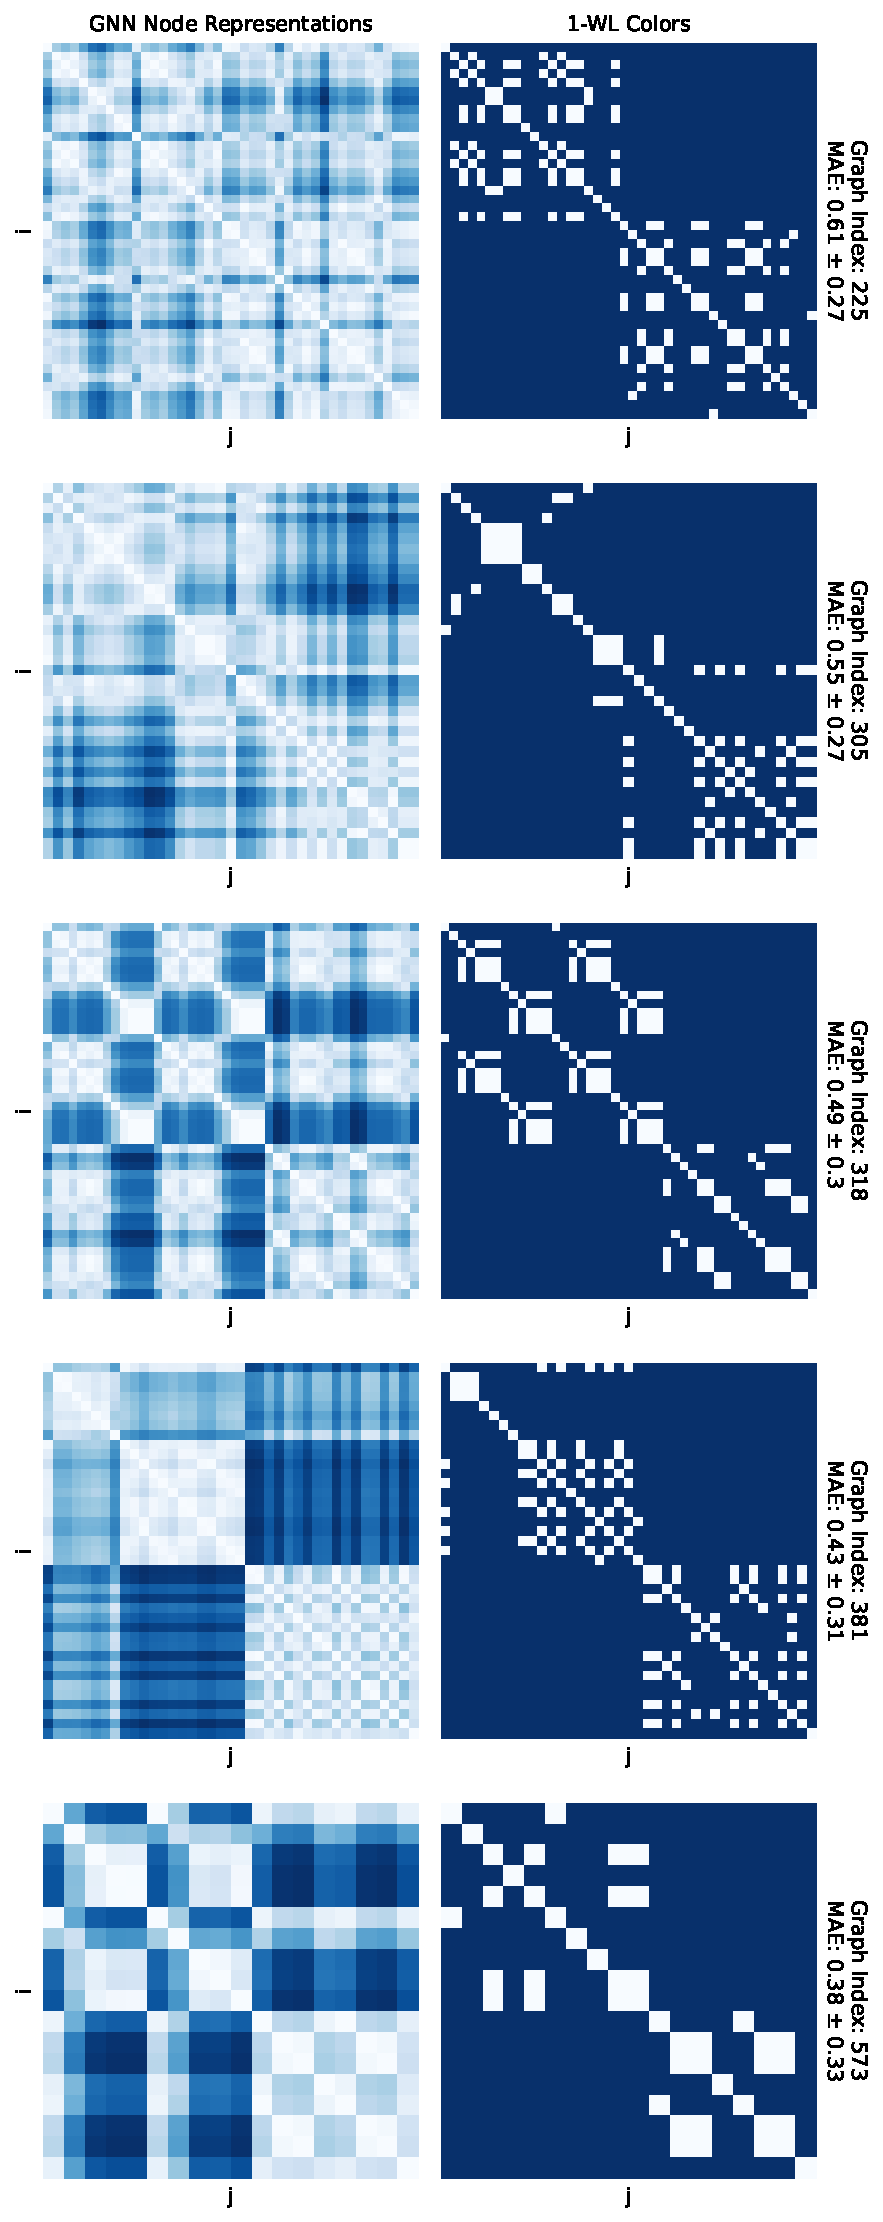
\includegraphics[width=\textwidth, left]{Figures/heatmaps_ENZYMES_0.pdf}
    \end{minipage}
    \hfill
    \begin{minipage}[b]{0.53007147296\textwidth}
        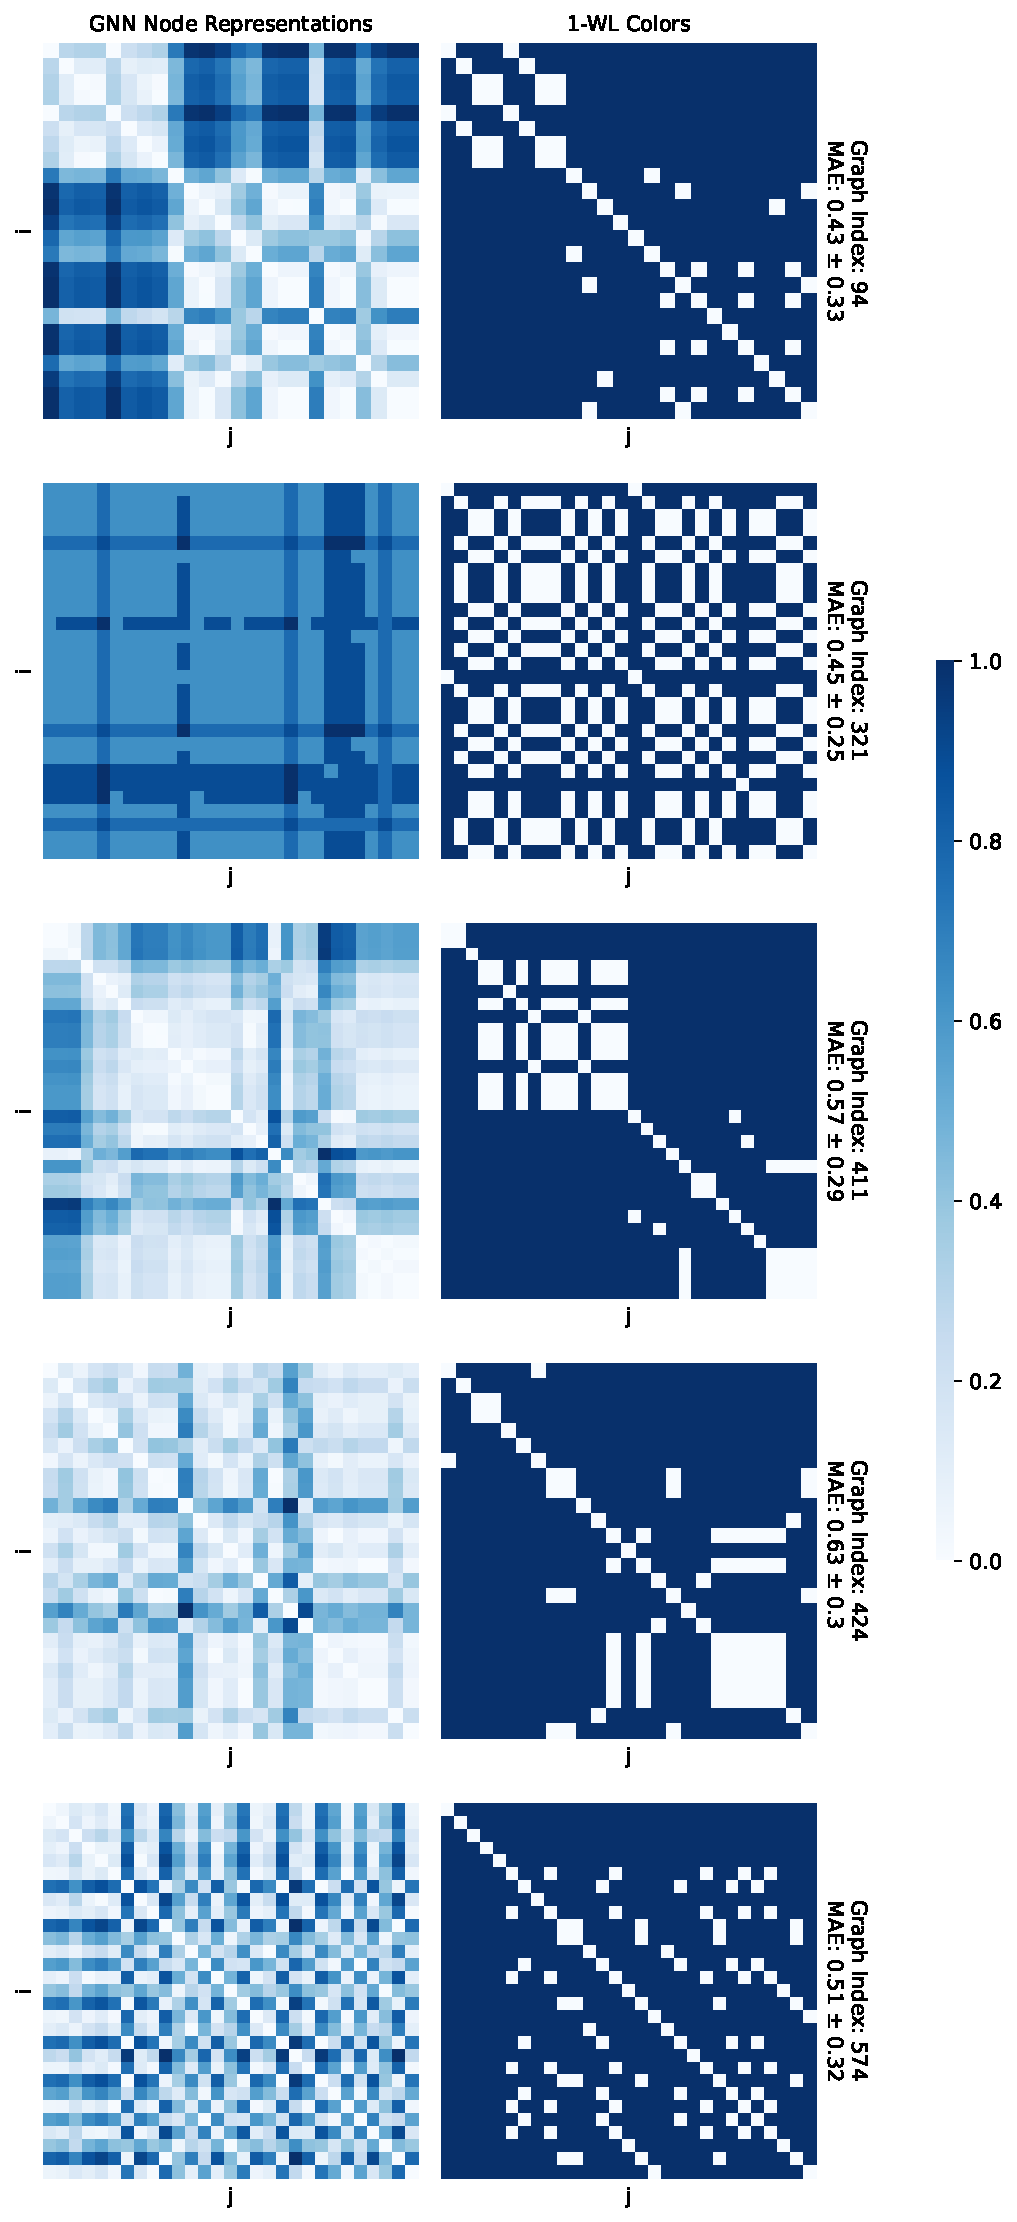
\includegraphics[width=\textwidth, right]{Figures/heatmaps_ENZYMES_1.pdf}
    \end{minipage}
    \hfill
    \caption{Visualizing the performance of the best performing GNN on the \textsc{Enzymes} dataset in approximating node colors computed by the 1-WL algorithm. The ten graphs shown are randomly sampled from the GNN's test set, and the 1-WL algorithm ran only for one iteration. The average error for the entire test set is $0.49 \pm 0.3$.}
\end{figure}

\begin{figure}[!ht]
    \centering
    \begin{minipage}[b]{0.45992852703\textwidth}
        \centering
        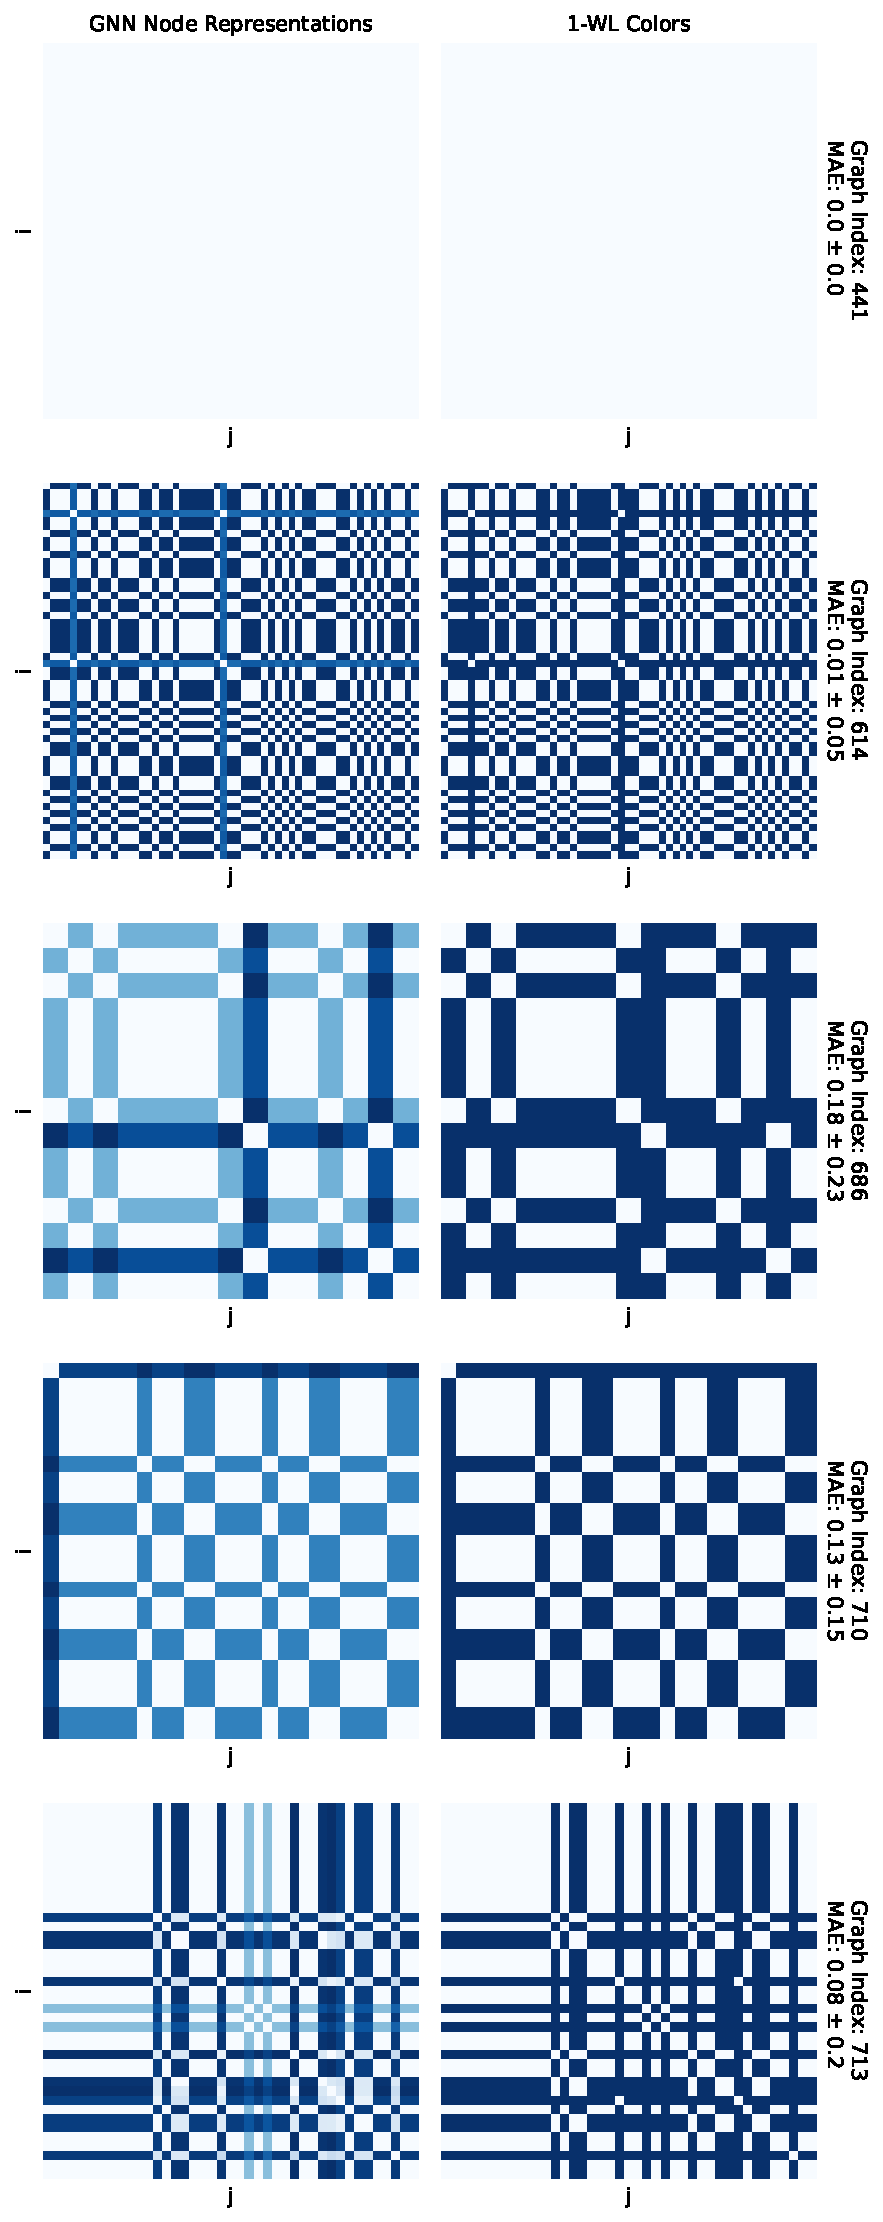
\includegraphics[width=\textwidth, left]{Figures/heatmaps_IMDB-BINARY_0.pdf}
    \end{minipage}
    \hfill
    \begin{minipage}[b]{0.53007147296\textwidth}
        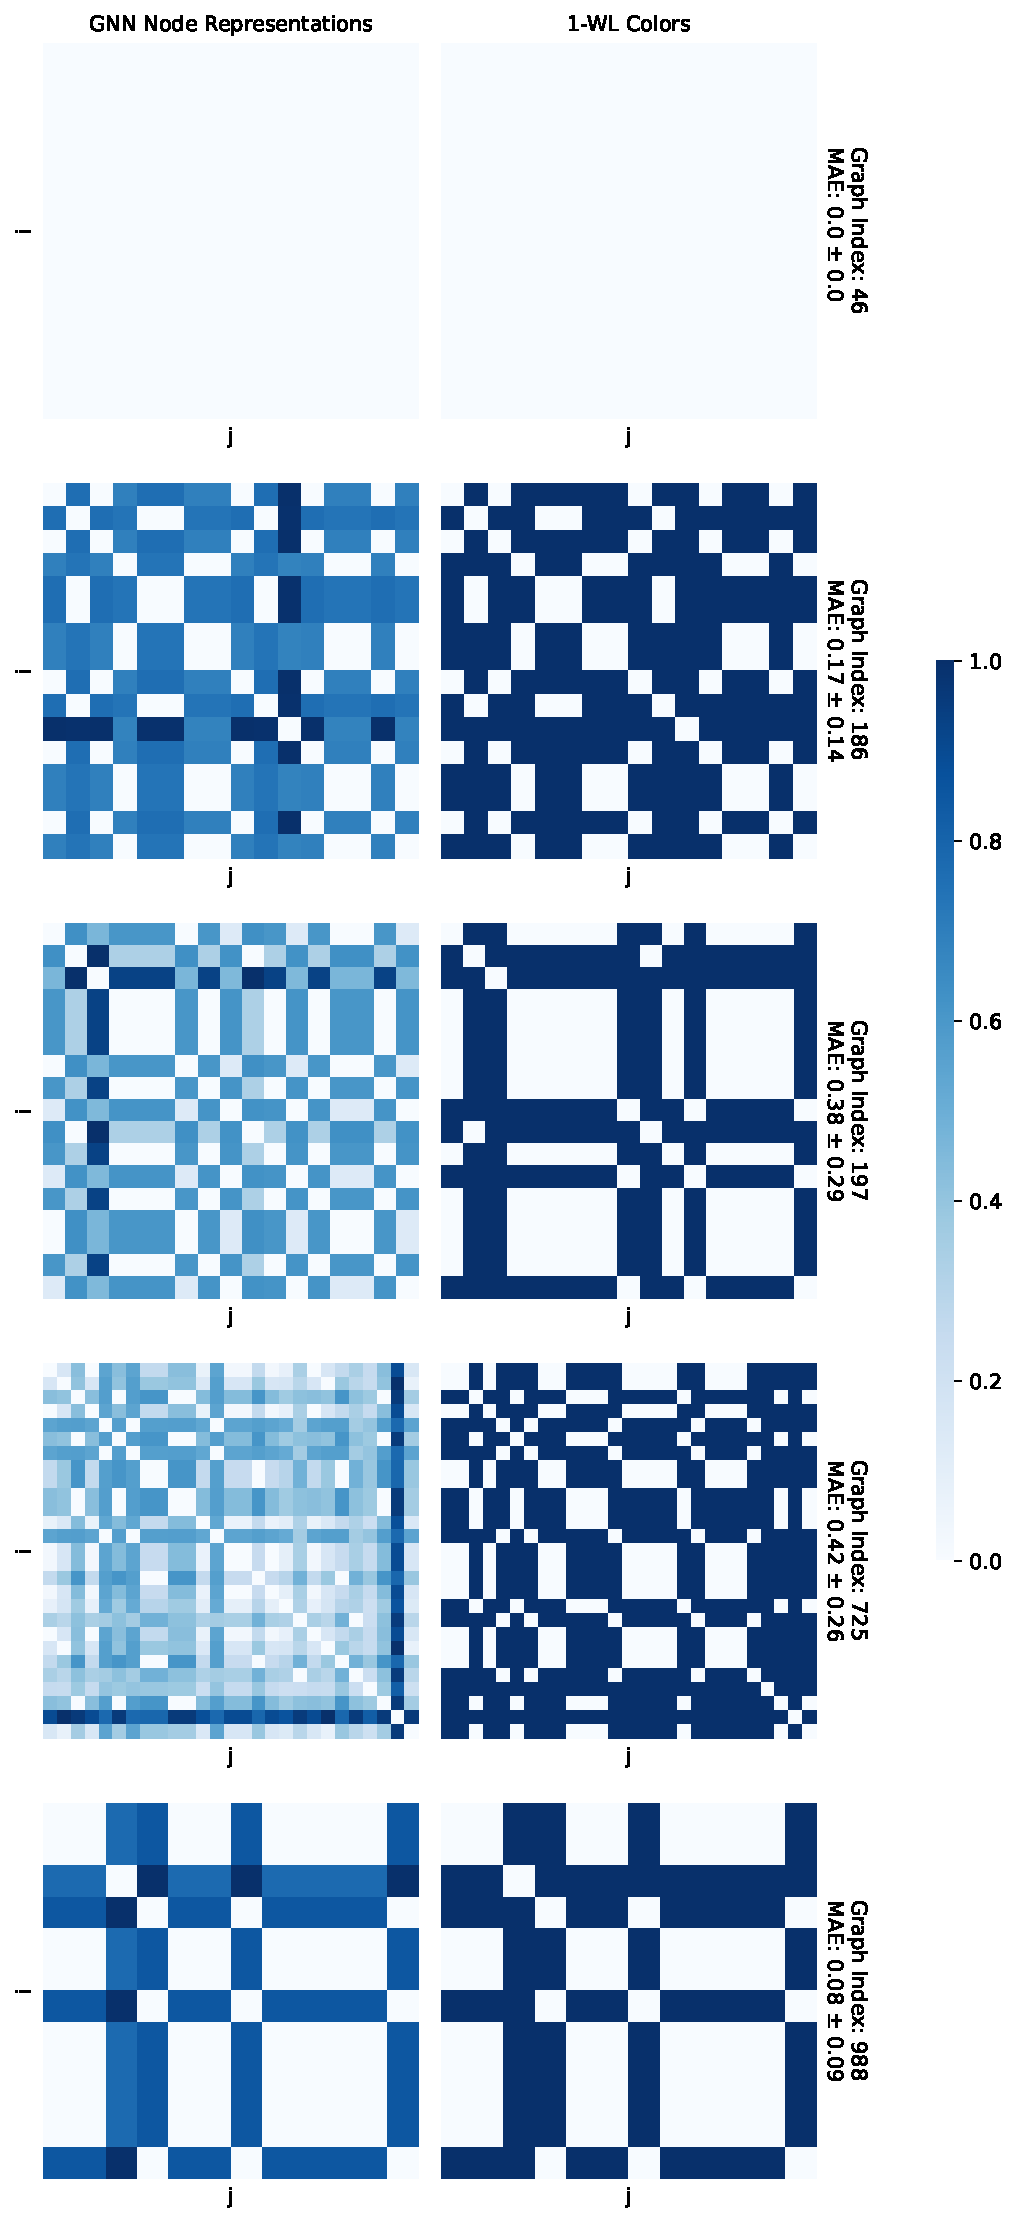
\includegraphics[width=\textwidth, right]{Figures/heatmaps_IMDB-BINARY_1.pdf}
    \end{minipage}
    \hfill
    \caption{Visualizing the performance of the best performing GNN on the \textsc{Imdb-Binary} dataset in approximating node colors computed by the 1-WL algorithm. The ten graphs shown are randomly sampled from the GNN's test set, and the 1-WL algorithm ran only for one iteration. The average error for the entire test set is $0.14 \pm 0.15$. \newline
    Note that \textsc{Imdb binary} does not contain any node features, so we artificially initialize each node feature with a one-hot encoding of its degree.}
\end{figure}

\begin{figure}[!ht]
    \centering
    \begin{subfigure}[b]{0.45992852703\textwidth}
        \centering
        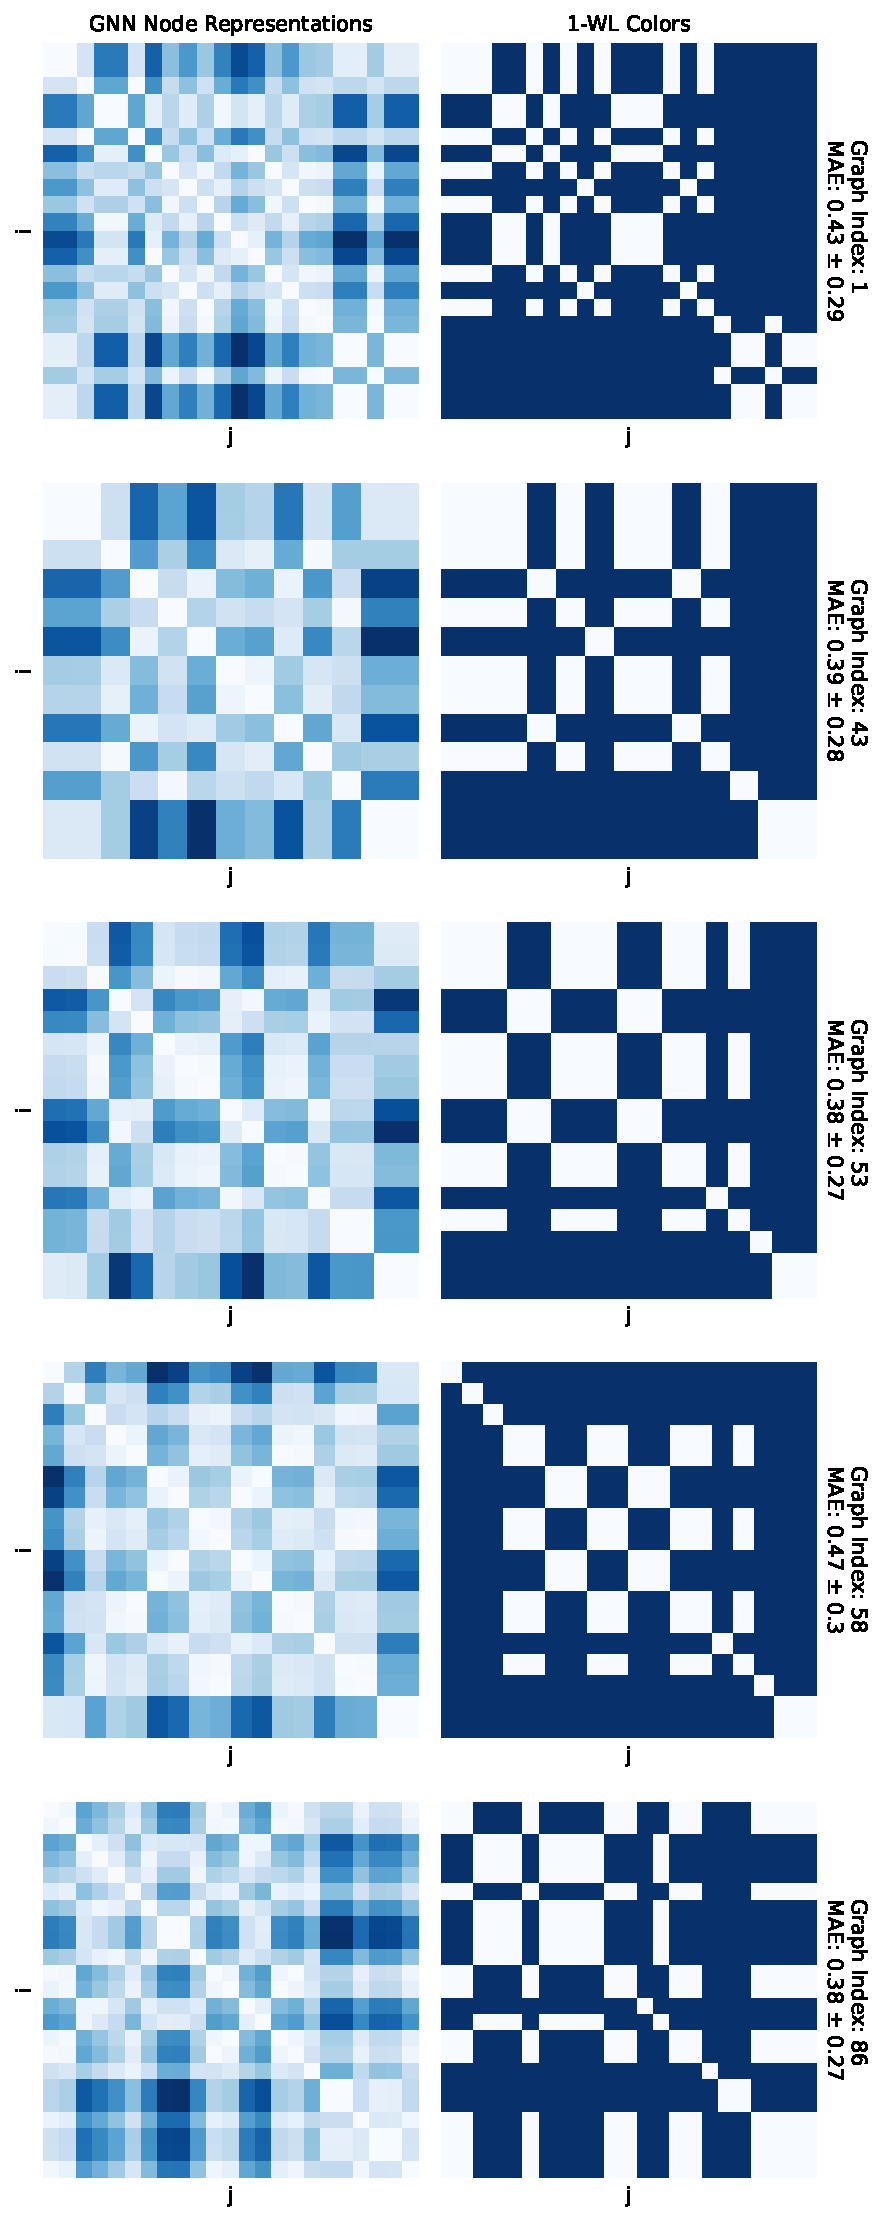
\includegraphics[width=\textwidth, left]{Figures/heatmaps_MUTAG_0.pdf}
    \end{subfigure}
    \hfill
    \begin{subfigure}[b]{0.53007147296\textwidth}
        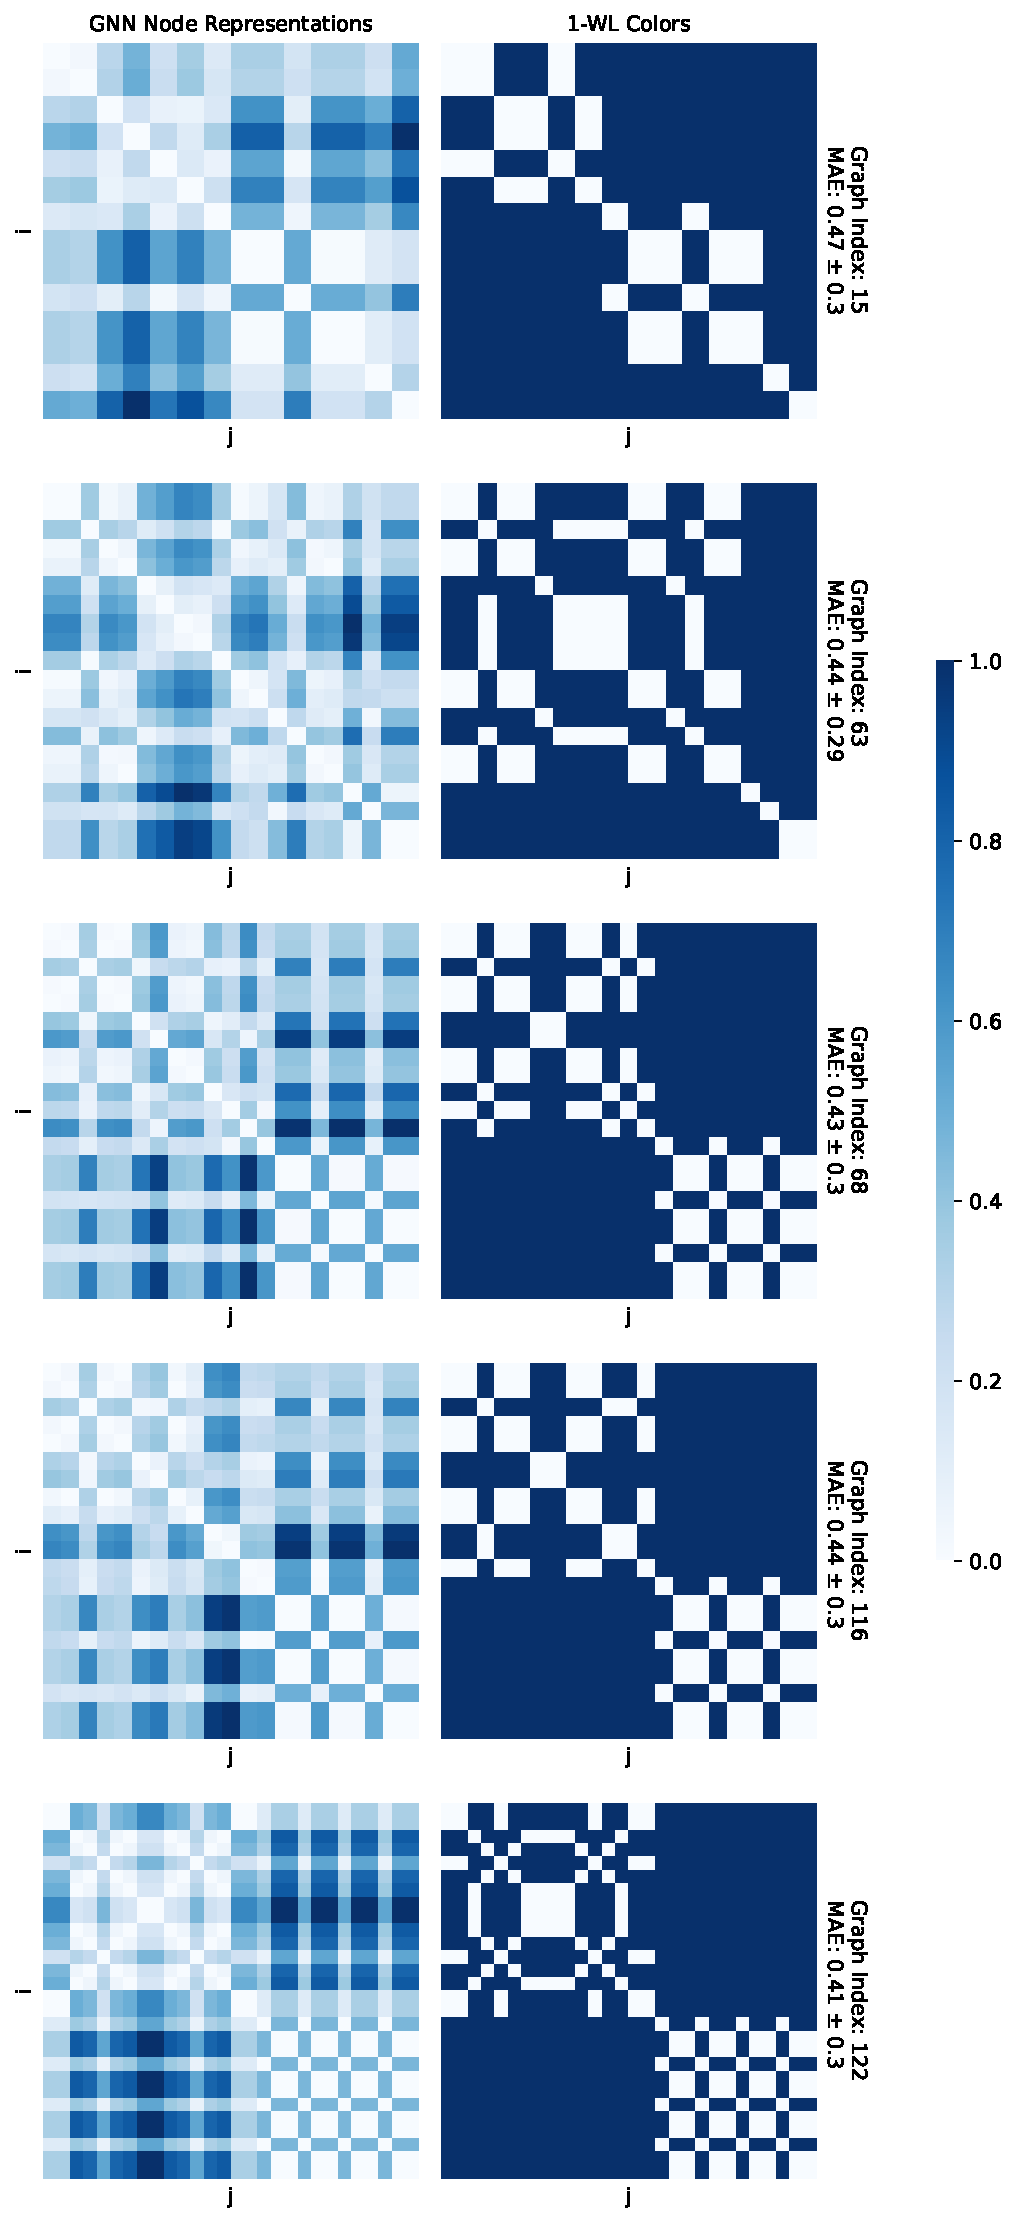
\includegraphics[width=\textwidth, right]{Figures/heatmaps_MUTAG_1.pdf}
    \end{subfigure}
    \hfill
    \caption{Visualizing the performance of the best performing GNN on the \textsc{Mutag} dataset in approximating node colors computed by the 1-WL algorithm. The ten graphs shown are randomly sampled from the GNN's test set, and the 1-WL algorithm ran only for three iteration. The average error for the entire test set is $0.42 \pm 0.29$.}
\end{figure}

\begin{figure}[!ht]
    \centering
    \begin{minipage}[b]{0.45992852703\textwidth}
        \centering
        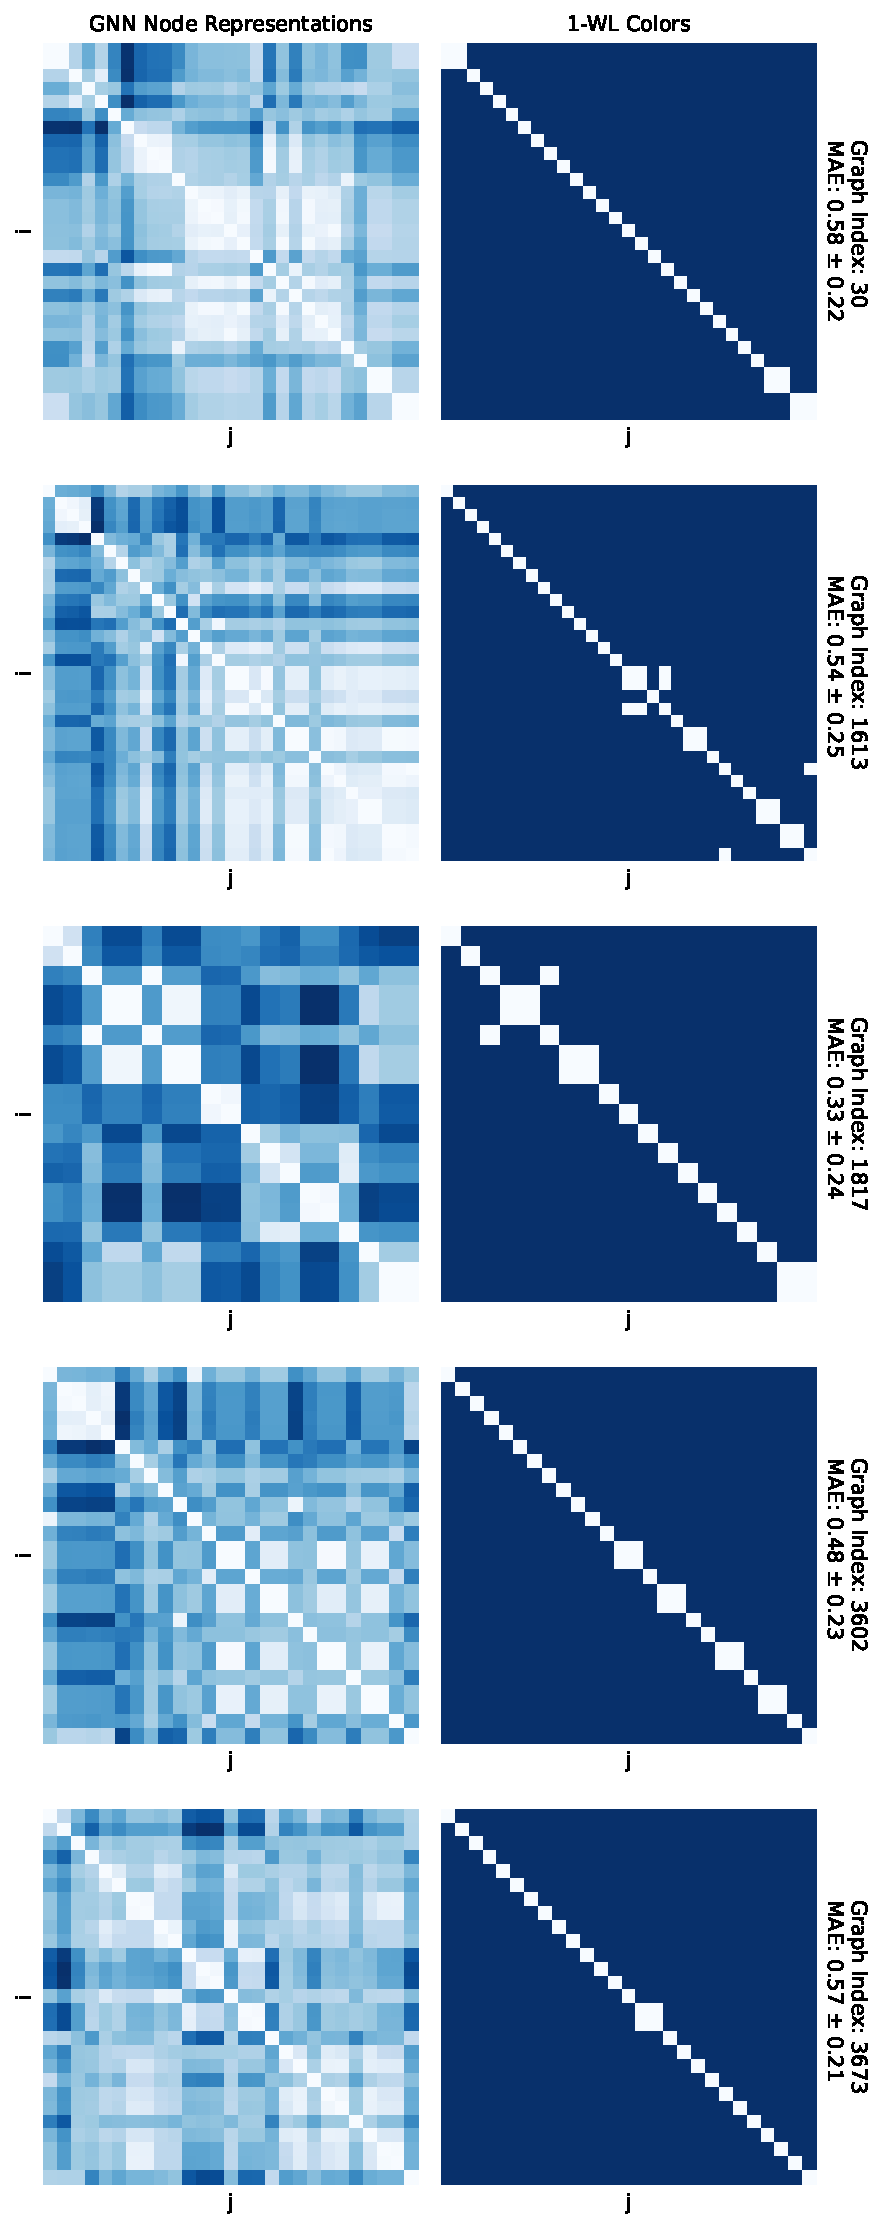
\includegraphics[width=\textwidth, left]{Figures/heatmaps_NCI1_0.pdf}
    \end{minipage}
    \hfill
    \begin{minipage}[b]{0.53007147296\textwidth}
        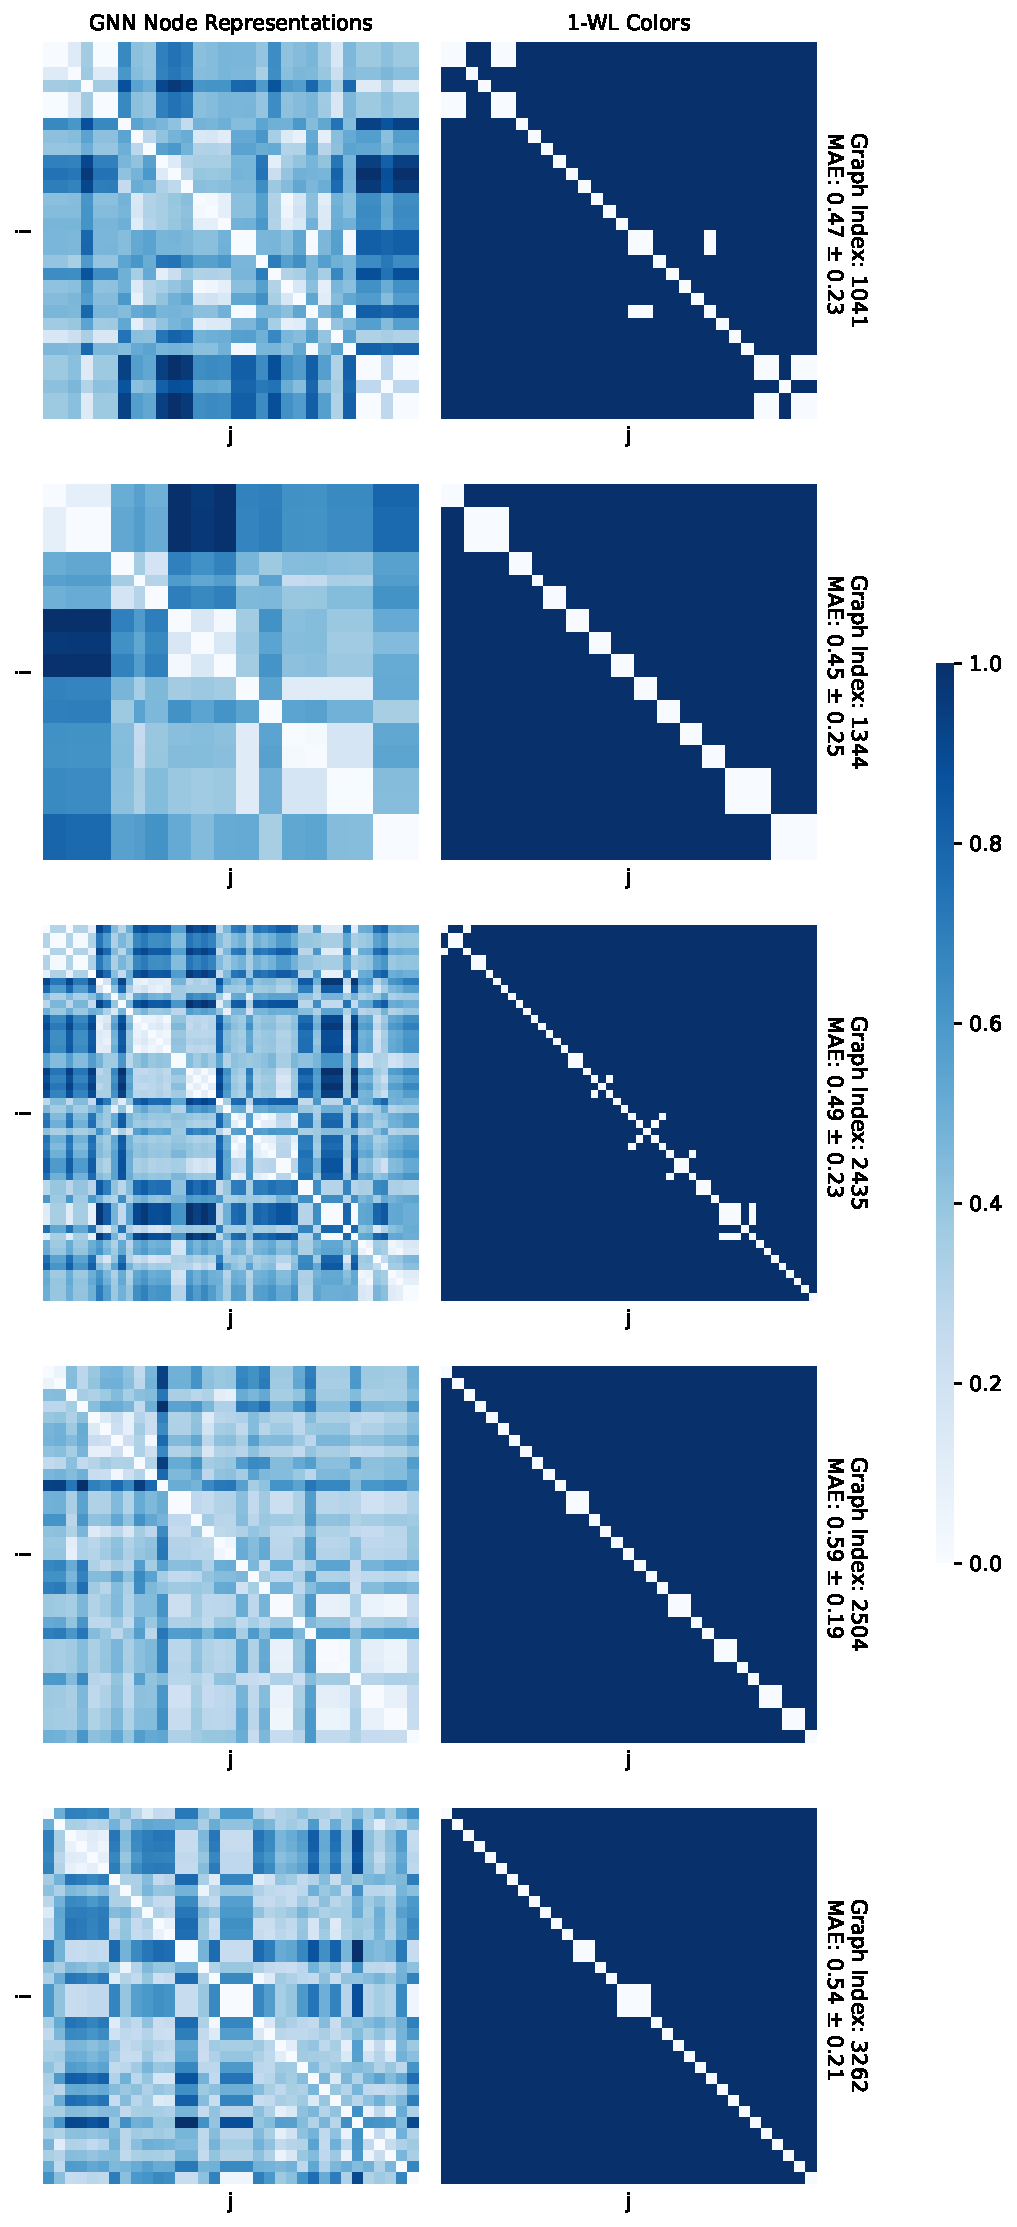
\includegraphics[width=\textwidth, right]{Figures/heatmaps_NCI1_1.pdf}
    \end{minipage}
    \hfill
    \caption{Visualizing the performance of the best performing GNN on the \textsc{Nci1} dataset in approximating node colors computed by the 1-WL algorithm. The ten graphs shown are randomly sampled from the GNN's test set, and the 1-WL algorithm ran only for three iteration. The average error for the entire test set is $0.50 \pm 0.24$.}
\end{figure}

\begin{figure}[!ht]
    \centering
    \begin{minipage}[b]{0.45992852703\textwidth}
        \centering
        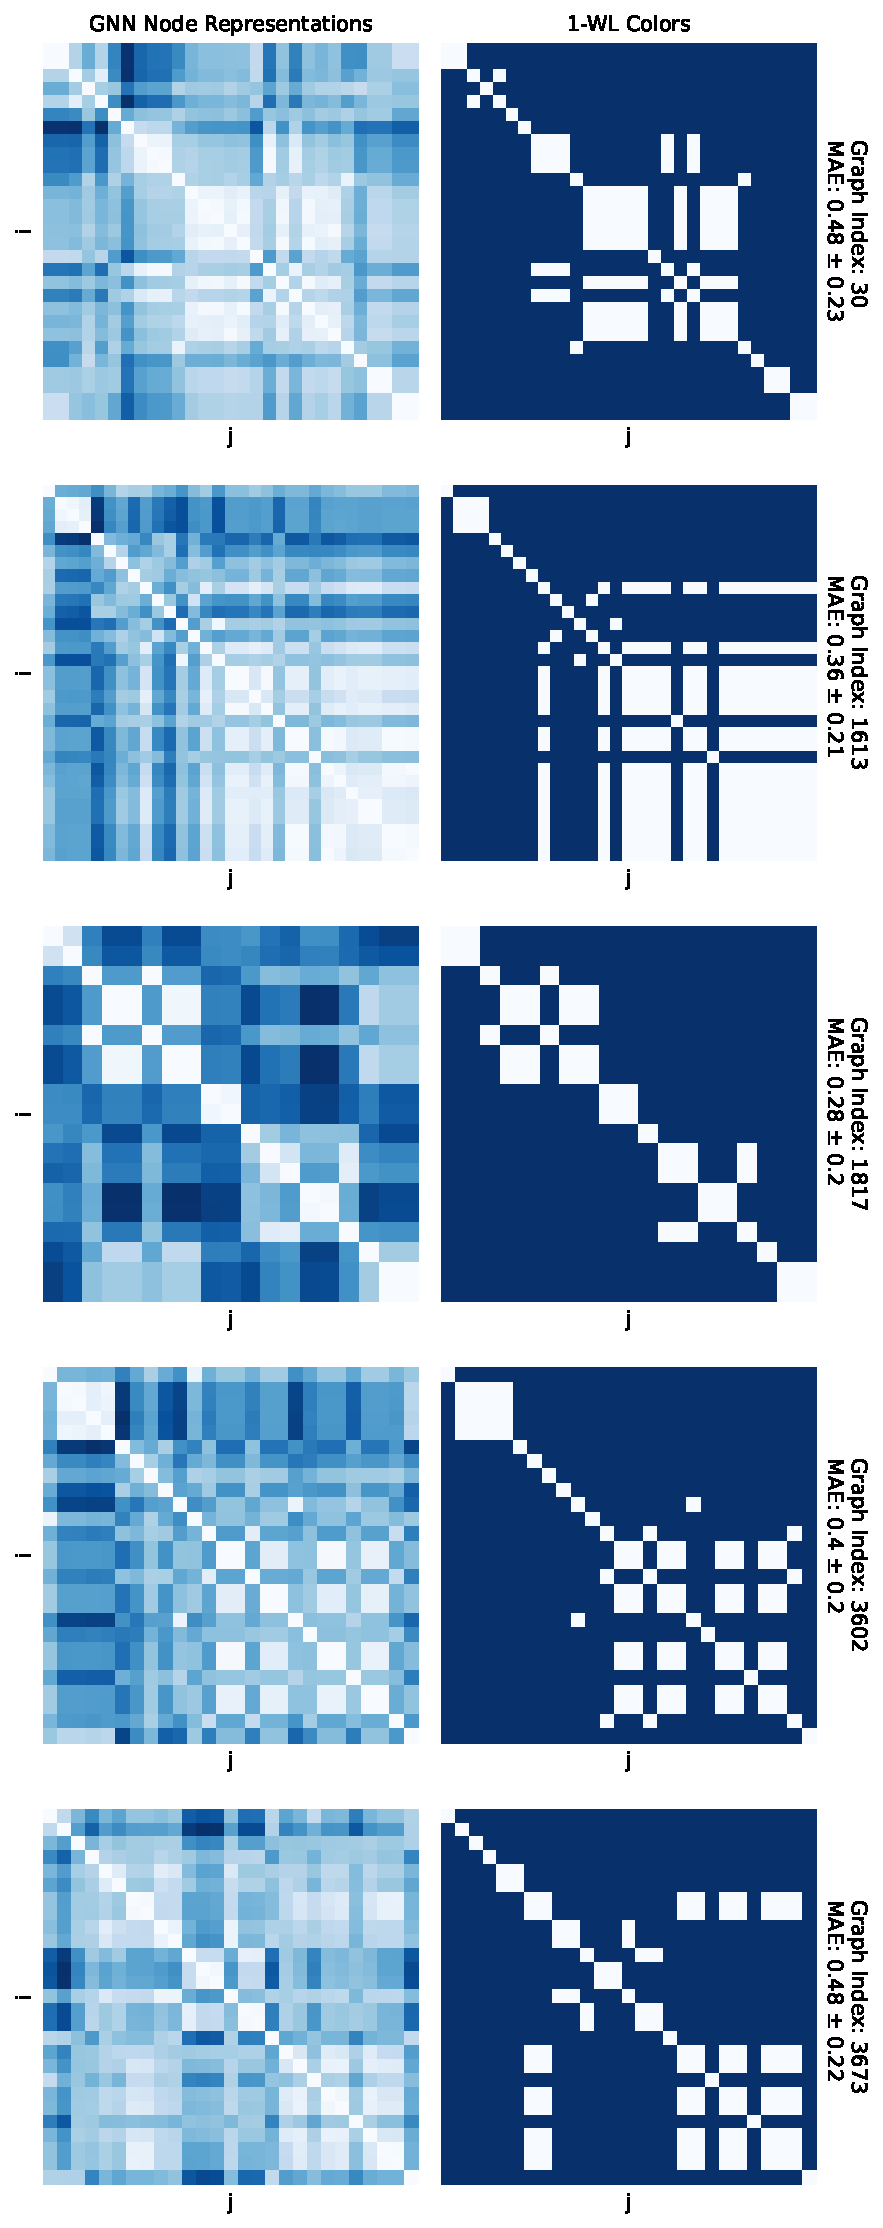
\includegraphics[width=\textwidth, left]{Figures/heatmaps_NCI1_0_k_wl_1.pdf}
    \end{minipage}
    \hfill
    \begin{minipage}[b]{0.53007147296\textwidth}
        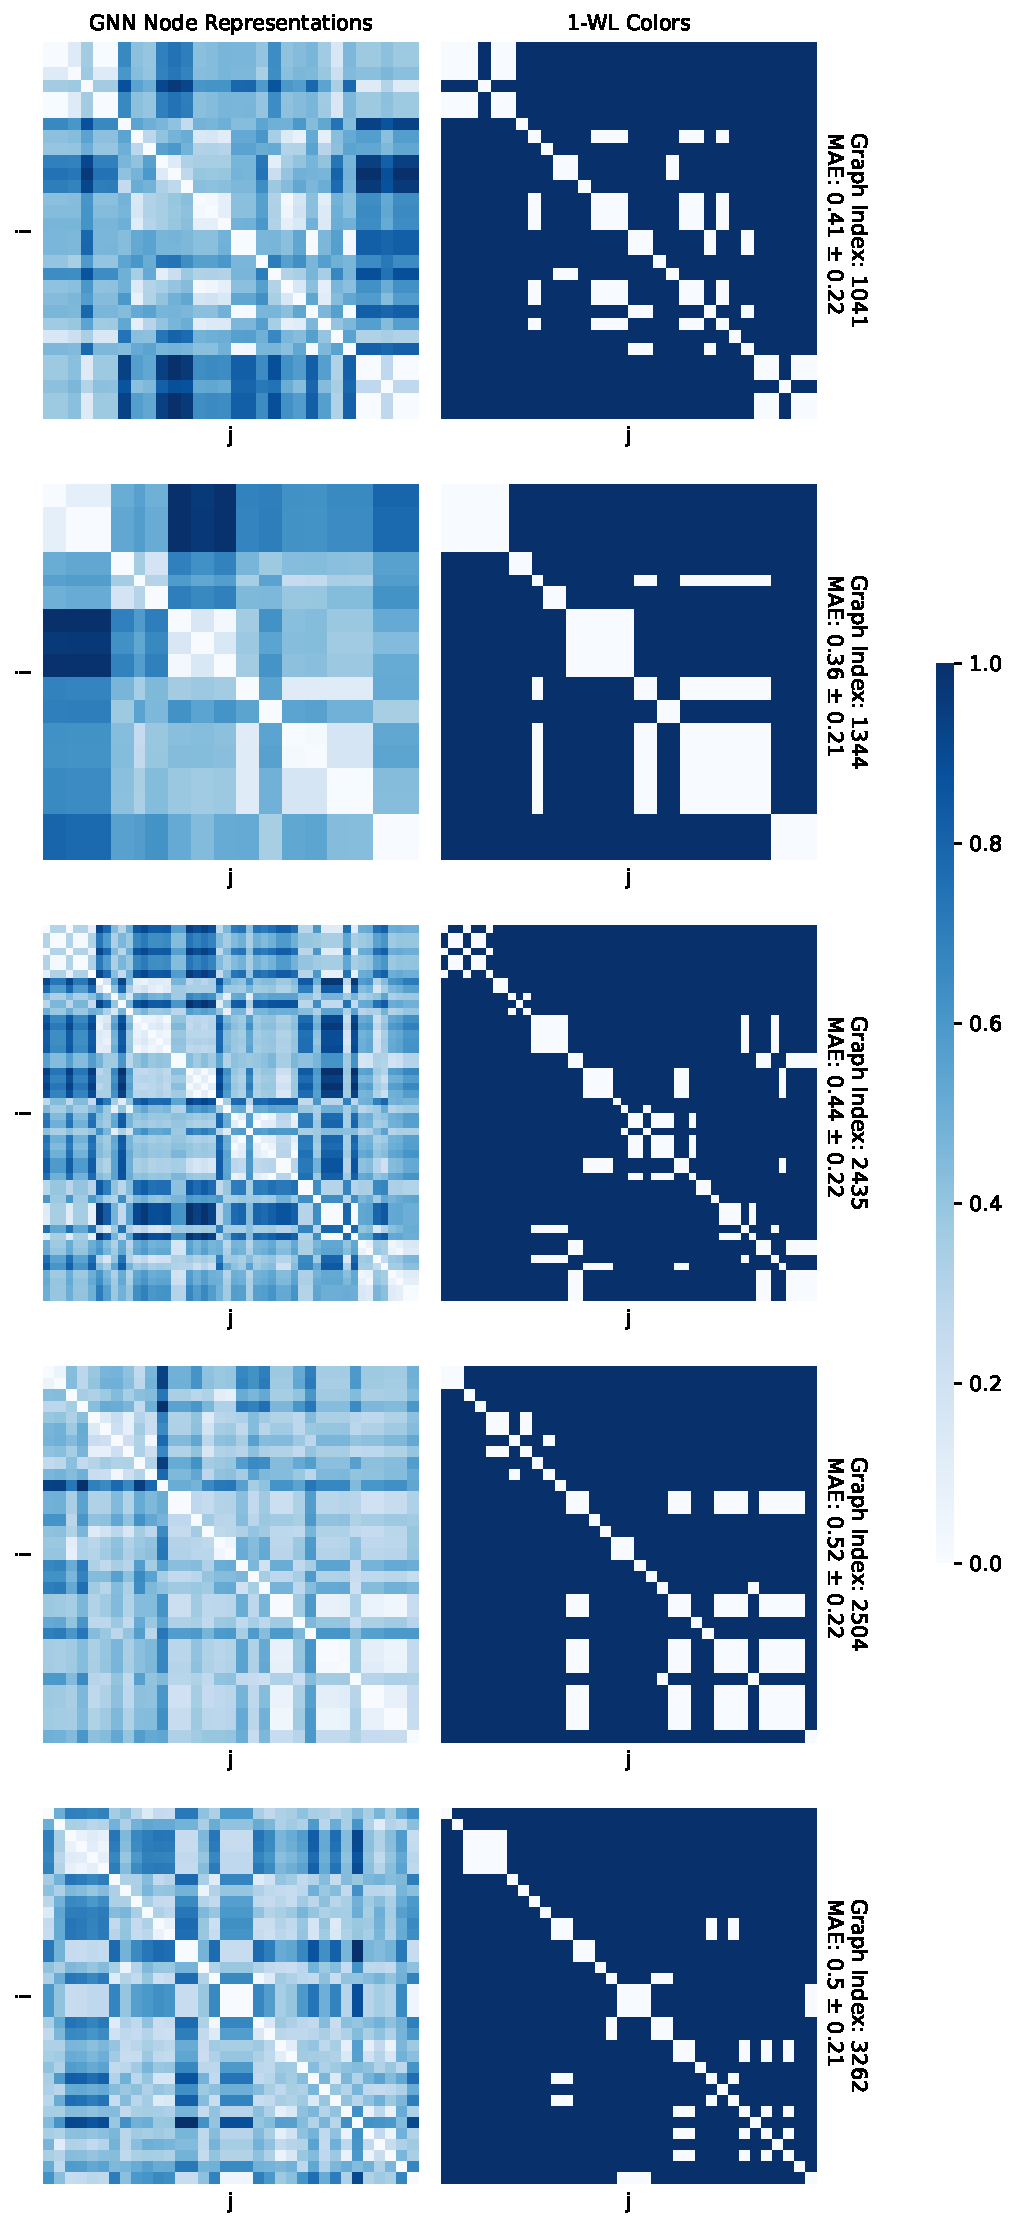
\includegraphics[width=\textwidth, right]{Figures/heatmaps_NCI1_1_k_wl_1.pdf}
    \end{minipage}
    \hfill
    \caption{Visualizing the performance of the best performing GNN on the \textsc{Nci1} dataset in approximating node colors computed by the 1-WL algorithm. The ten graphs shown are randomly sampled from the GNN's test set, and the 1-WL algorithm ran only for one iteration. The average error for the entire test set is $0.42 \pm 0.22$.}
\end{figure}

\begin{figure}[!ht]
    \centering
    \begin{minipage}[b]{0.45992852703\textwidth}
        \centering
        \includegraphics[width=\textwidth, left]{Figures/heatmaps_PROTEINS_0.pdf}
    \end{minipage}
    \hfill
    \begin{minipage}[b]{0.53007147296\textwidth}
        \includegraphics[width=\textwidth, right]{Figures/heatmaps_PROTEINS_1.pdf}
    \end{minipage}
    \hfill
    \caption{Visualizing the performance of the best performing GNN on the \textsc{Proteins} dataset in approximating node colors computed by the 1-WL algorithm. The ten graphs shown are randomly sampled from the GNN's test set, and the 1-WL algorithm ran only for one iteration. The average error for the entire test set is $0.49 \pm 0.26$.}
\end{figure}


\end{document}
